%\documentclass[fontsize=11pt, appendixprefix=true]{scrreprt}
\documentclass[11pt]{report}
\usepackage{tocloft}
%\renewcommand{\cftpartleader}{\cftdotfill{\cftdotsep}} % for parts
%\renewcommand{\cftchapleader}{\cftdotfill{\cftdotsep}} % for chapters
\renewcommand{\cftsecleader}{\cftdotfill{\cftdotsep}} % for sections, if you really want! (It is default in report and book class (So you may not need it).

% appendixprefix: hogy odaírja, hogy "Függelék A", ne csak "A"
%\usepackage[english, magyar]{babel}                        % nyelvi csomag
\usepackage[T1]{fontenc}                                   % ékezetes betűknél is legyen automatikus elválasztás
\usepackage[utf8]{inputenc}                                % ékezetes betűk kezelése
\usepackage{lmodern}                                       % alapértelmezett betűtípus ne legyen pixeles
\usepackage{mathtools}                                     % képletekhez kell
\usepackage[backend=biber, sorting=anyt]{biblatex}           % bibliográfia
\addbibresource{bscthesis.bib}

\usepackage{graphicx}                                      % képek beszúrása
\graphicspath{ {images/} }
\usepackage[export]{adjustbox}                             % ez az ITK logó pozicionálásához kell
\usepackage[margin=2.5cm, bindingoffset=1.25cm]{geometry}  % margók
\usepackage[onehalfspacing]{setspace}                      % másfeles sorköz
\usepackage[hidelinks, unicode, pdfusetitle]{hyperref}     % kattintható tartalomjegyzék és hivatkozások
\usepackage{bookmark}                                      % PDF könyvjelzők
\usepackage{csquotes}                                      % a bibliográfiában megfelelően legyenek formázva az idézőjelek
\DeclareQuoteAlias{german}{magyar}

% Kódrészletekhez ajánlom
\usepackage{listings, scrhack}
\usepackage{sourcecodepro} % egy jó betűtípus
\lstset{captionpos=b, numberbychapter=false, basicstyle=\ttfamily, showstringspaces=false, columns=fullflexible}
% Kódrészletek magyar stílusú számozása
\renewcommand\lstlistingname{kódrészlet}
\makeatletter
\renewcommand\fnum@lstlisting{\ifx\lst@@caption\@empty\else\thelstlisting.~\fi\lstlistingname}%
\makeatother
% Nyilatkozathoz két parancs definíciója
\newcommand{\pushtobottom}{\vspace*{\fill}}
\newcommand{\signatureline}[1]{\begin{flushright}
	\vspace*{.5cm}\par\noindent\makebox[2.5in]{\hrulefill}
	\par\noindent\makebox[2.5in][c]{#1}
	\end{flushright}
}


% Ezeket írd át!
\author{Csaba Botos}
\title{Building, testing and visualizing neural networks from scratch}
\date{2016}
%\subject{A thesis submitted for the Council of Scientific Students’ Associations}
%\publishers{Advisor:\\PhD.\ István Z. Reguly}

\usepackage{titlesec}

% Chapter customization
\renewcommand\thesection{\arabic{section}}

\titleformat{\chapter}[block]
  {\normalfont\Huge\bfseries}{\thechapter.}{1em}{\huge}

% For quotes
\usepackage{epigraph}
\setlength\epigraphwidth{0.7\textwidth}
\setlength\epigraphrule{0pt}

\begin{document}
%%%%%%%%%%%%%%%%%%%%%%%%%%%%%%%
%% BEVEZETÉS


\includegraphics[valign=m]{ITK_logo} \parbox[c]{\textwidth}{Pázmány Péter Catholic University\newline Faculty of Information Technology and Bionics}
\vspace*{\fill}

{\let\newpage\relax\maketitle}
\vspace*{\fill}
\begin{center}
A thesis submitted for the Council of Scientific Students’ Associations\\
Advisor: PhD.\ István Z. Reguly
\end{center}
\clearpage


\chapter*{Abstract}

Recently a special branch of Machine Learning, a model based on living organic systems called Deep Neural Networks is overtaking previous paradigm of algorithmic problem solving. 
It gained larger attention when better results were achieved than task-specific, handcrafted models in feature extraction. 
The reason behind its success is its scalability: the latest architectures are able to exploit the capacity of cutting-edge GPU hardware since the abstraction of the data is accomplished by succeeding neural nodes performing elementary operations, which can be easily parallelized.

It is of the utmost importance to understand the main concept of such networks to contribute to the breakthroughs of the fourth industrial revolution. 
To this purpose, building a framework from the base unit blocks of the newest models is the best introduction to Machine Learning. 
In my research I have disassembled black-box represented networks to the very basic, intuitive level and reorganized it in object-oriented manner, where each neural layer is treated as an entity derived from a common ancestor, therefore information flow and processes of the system are easily traced. 
My design and implementation is based on the principals of the components used by networks built for ImageNet classification, such as Convolutional, ReLU, Max-Pooling, Fully-Connected, Dropout, DropConnect, Softmax and k-Winner-Takes-All layers.
Furthermore, the following training methods and policies were adapted: cross validated, mini-batch, on-line, $L_p$ regularized and basic Stochastic Gradient Descent training.

For testing the framework, the parameter space of Fully Connected networks was exhaustively explored. 
After training and evaluating sessions - mainly performed on the MNIST and self-acquired datasets - the results were gathered to analyze the performance of different architectures. 
For further investigation the best performing models  were compared to each other to find pros and cons of different capacity, layout and training of networks.

Besides architectural experiments, a non-trivial task targeted by many recent research of visualizing the inner representation of information, understanding transient activation patterns was studied as well.
Previously mentioned candidate networks were also visualized individually to retrieve information about characteristics of the processes in their Hidden Layers.
My implementation proposes a simplification of the DeconvNet derived from Gradient Ascent, an efficient algorithm to reveal patterns recognized by nodes in the hidden layers of Neural Networks, to produce adversarial input samples.
\addcontentsline{toc}{chapter}{Abstract}
\clearpage

\chapter*{Declaration}
I, Botos Csaba, declare that this thesis titled 'Building, testing and visualizing neural networks from scratch', and the work presented in it are my own. I confirm that:

\begin{itemize} 
\item This work was done wholly or mainly while in candidature for a research degree at this University.
 
\item Where any part of this thesis has previously been submitted for a degree or any other qualification at this University or any other institution, this has been clearly stated.
 
\item Where I have consulted the published work of others, this is always clearly attributed.
 
\item Where I have quoted from the work of others, the source is always given. With the exception of such quotations, this thesis is entirely my own work.
 
\item I have acknowledged all main sources of help.
 
\item Where the thesis is based on work done by myself jointly with others, I have made clear exactly what was done by others and what I have contributed myself.

\end{itemize}
\signatureline{Signature}
\clearpage  % Declaration ended, now start a new page

\tableofcontents
\clearpage

\chapter{Introduction}
\section{Overview}


\epigraph{\textit{No one knows what the right algorithm is, but it gives us hope that if we can discover some crude approximation of whatever this algorithm is and implement it on a computer, that can help us make a lot of progress.}}{\rightline{{\rm --- Andrew Ng}}}

Every time we are interacting with our environment, we get closer to understand it %still the closer we are the less we understand. 
However, as a byproduct, questions arise for which pure logical (mathematical) solution is not available, or the problem is larger than to be solved by current ones.
Luckily we can always turn back to nature for inspiration: biological systems have proven their efficiency, therefore their functions worths to be further analyzed even if there could be theoretically a better way to tackle obstacles. 
One of the many branches of artificial intelligence, Neural Network is based on the nerve systems of living organisms which is capable of self-learning.

Such a simple paradigm is playing a fundamental role in boosting the industry and researches of today, because introducing Machine Learning to any field of life results in great leap forward. 
Thanks to the recent technological advancements, even with the current computational capacity of a personal computer one can get encouraging results by simply exploring the core principles of the topic.

\textbf{Main motivation.} Using outer libraries \cite{TF, torch, caffe}, without diving deep into mathematical proofs, treating neural networks as black-boxes thousands of useful applications \cite{haykin2004comprehensive} are made. 
On the other hand, building such architectures from the very basics helps to clarify how simple units might be organized, taught \cite{werbos1994roots}, and function \cite{hornik1989multilayer} as a large system. 
As complexity arises, the processes in the network becomes unclear and brings (yields?) the question: what is the purpose of each node? Methods to visualize how activation patterns formulate, and what information is held within them has been already investigated \cite{yosinski2015understanding}, and applied to improve performance \cite{zeiler2014visualizing}. My studies are mainly rely on recent publications, and researches in field of computer vision. The design of my own Deep Learning framework library is influenced by hot off press tutorials \cite{Goodfellow-et-al-2016-Book, deeplearningdotnet, nnsdl, stanfordlectures, gibiansky} and open-sources \cite{TF, torch, caffe} available for anyone. 

\textbf{Primary goal.} With my work I intend to bring closer, and demystify cutting-edge concepts of applied neural networkings for larger audiences. 
On related works and case studies I want to show what can be done by simply starting from the drawing board

\section{Importance of understanding}
\section{Thesis outline and contributions}






%
%\section*{Biological Motivation}
%\section*{Real Life Applications}
%\section*{Black Box representation}
%\section{The Perceptron model}
%\section{Importance of understanding}
%\section{Visualization}
	%2-5 oldal
\clearpage
\chapter{Literature}


% VÉGÉRE!
Considering course slides \cite{stanfordlectures, oxfordlectures} and textbooks \cite{Goodfellow-et-al-2016-Book, werbos1994roots} of established universities, popular websites \cite{deeplearningdotnet, pedregosa2011scikit}, blogs \cite{gibiansky, karpathyblog} and vlogs \cite{vlog1} on Artificial Neural Networks one might find it hard to find a good point to start. 
Some content may offer formal description of the general machine learning problem, others try to clarify through analogies with the biological nerve system.
Tutorials, which I have found interesting, and the most helpful, had several common features which are important to adapt, when designing a neural network library. 
Generally these common attributes are the following: 
they intend to be \emph{simple} as possible, 
have many \emph{intuitive} examples and analogies,
their \emph{interpretations} are not restricted to either universal approximators, or nervous systems of living organisms, but combines both aspect.		% minimum 10 oldal
\clearpage
%% BEVEZETÉS
%%%%%%%%%%%%%%%%%%%%%%%%%%%%%%%
%% TARTALOM
\chapter{Design and Implementation}\label{cp:design}

\epigraph{\textit{... where in this snippet $W1$ and $W2$ are two matrices that we initialize randomly. We're not using biases because meh.}}{\rightline{{\rm --- Andrej Karpathy}}}

After researching literature on building libraries from scratch, analyzing pet project source-codes \cite{convnetjs, gibianskysource} and dozens of implementations of professional libraries \cite{TF, caffe, torch},
I concluded that the best way to acquire an in-depth understanding of neural networks is to build my own Deep Learning framework.
This way I had a chance to understand why novel solutions in Machine Learning are formed the way they are.
I also gained insight into what main paradigms are popular libraries based on, such as \emph{computational graphs, parallel processing}, 
and what trade-offs can be made between \emph{computational cost} and \emph{memory usage}, between robustness and plasticity.
Most thankfully, by starting from scratch I have faced situations when theoretical formulas had to be translated into exact working code, which was an important challenge for me.

\paragraph{Goals.} My main objectives when writing code were the following:
\begin{itemize}
    \item[] to make a library that can be extended further
    \item[] open-source, so it can be forked by anyone interested in developing it
    \item[] to make it modular therefore make its usage independent of the task
    \item[] use the fewest possible technical tricks for sake of simplicity
    \item[] to stay as close to pure mathematical formulation of the classical paradigms as possible
    \item[] put emphasis on ease of use and understanding
\end{itemize}
\paragraph{Disclaimer.} Apart from \textbf{NumPy} and its complementary package \textbf{SciPy}, no external libraries and dependencies are used in the implementation. 
I want to emphasize that this work was not written to compete with contemporary state-of-the-art frameworks, rather to help perceive the general ideas behind novel researches, and to encourage interested fellows to carry out researches on their own.
\clearpage
\section{Choice of design pattern and language}

The formulas of classical neural networks, whose nodes are organized into
 lattices forming a Directed Acyclic Graph, show minor variance in
 contents of independent sources. Still their common point that they rely
 on basic vector algebra and functional analysis, therefore considering
 arrays representing general mapping functions, as their core building
 blocks is a paradigm which would not interfere with the current formal
 and informal descriptions of deep learning.

\subsection{Disassembling a universal approximator}
Thinking of a neural net as a function \(\mathcal{F}\), is implicitly a black-box representation of the paradigm.
Users of different applications which offer feature detection, segmentation, prediction, etc. are using this function without knowing what exactly happens behind the curtains. 
Further investigating $\mathcal{F}$, we can constrain it to have a DA computational graph, also to have the nodes of the graph arranged to lattices.
Practically it means that the perceptrons making up the layer \(l\) are strictly projecting $F_l$ their \textbf{inputs} 
$ x_l \in \mathbb{R}^N $ \emph{forward} to scalars, which if all perceptrons are evaluated in parallel, forms the 
\textbf{output} $y_l \in \mathbb{R}^M$, have no feedbacks and loops. 
This projection of layer $l$ can be written as $y_l = F_l(x_l)$. 
Intuitively the input of the next $(l+1)^{th}$ layer will be the output of the previous layer:
$x_{(l+1)} = y_l$.
For the sake of simplicity I excluded Recurrent Networks from the space of $\mathcal{F}$, but later the definition can be extended for vanilla recurrent networks and LSTM networks as well.

\subsection{Language} Keeping in mind that using a general high-level language (like MATLAB) can yield poor computational efficiency, making benchmarks, testing and applications ponderous.
Also considering a low-level language (like C) 
would distract us from the main goal, all 
the time is spent on optimizing further and 
further the basic algorithms, and usage usually 
results in boilerplate codes. 
Either way it would make the implementation unclear for those, who did not participate in the designing of the library.
I wanted to chose a language which offers an optimal solution for this challenge, is flexible, well documented and simple enough for newbies to catch up.
Because of the support of both object-oriented and procedural approaches and offering the above, I chose Python.

\subsection{Design pattern} While designing blueprints of the implementation, I examined the Neural Networks as universal approximators in a \textsc{top-down} manner.
I have disassembled them to basic blocks, abstracting the function of each level.
Later I used these units in \textsc{bottom-up} approach to create an object-oriented hierarchic model that realizes simple operations and is well defined on every level: granting a universal interface to be further extended.


\section{Single Layered networks}
For example if a small picture is given to a person, he or she guesses about it. If that person is told that there are four classes, 
like \emph{Car, Plane, Cat, Kid}, he can tell how likely it is that 
the given picture falls in that class, so he can give a so-called \emph{confidence parameter}.
Patterns which are associated with cats may be associated with kids too, but is unlikely to be associated with planes. Deciding whether a pattern improves the confidence on each class or not, yields a \textbf{sign} for the given pattern, and the measure how strongly it influences the likelihood is called the \textbf{weight} of the pattern.
In \emph{neural networks} there are small nodes based on the biological model of neurons, that is responsible for recognizing and weighting the patterns. These nodes are called \textbf{perceptrons}. 

\subsection{Defining the Perceptron} 
Let $x$ be preprocessed information, the perceptron $\mathbf{P}$ decides which parts of it are important in recognizing a cat: having a corresponding weight with large magnitude, and which of them are irrelevant: having a weight with magnitude close to zero. 
Therefore a \emph{perceptron} has a weight $w_i$ for each input $x_i$ and its transient state can be now formally written:
$$
	\mathbf{P}_{transient}=\sum_i x_i w_i
$$
Which can be also rewritten as the inner product of $\mathbf{x}$ and $\mathbf{w}$

$$
	\mathbf{P}_{transient}= <\mathbf{x} \;,\; \mathbf{w}>=\mathbf{x}^T\mathbf{w}
$$
In the following examples perceptrons will be arranged in a special way, to form a \textbf{Feed Forward} network, meaning that the information flow will occur in a direct way, without feedback - see figure \ref{fig:ff}.
However wiring many perceptrons together results in a numerically unstable system, caused by the lack of any restriction on the magnitude of the weights.
Regularization addresses exactly this problem, implicitly making the network less likely to simply memorize pictures, or only respond to samples from the training set -- the problem of overfitting.

\begin{figure}
	\centering
	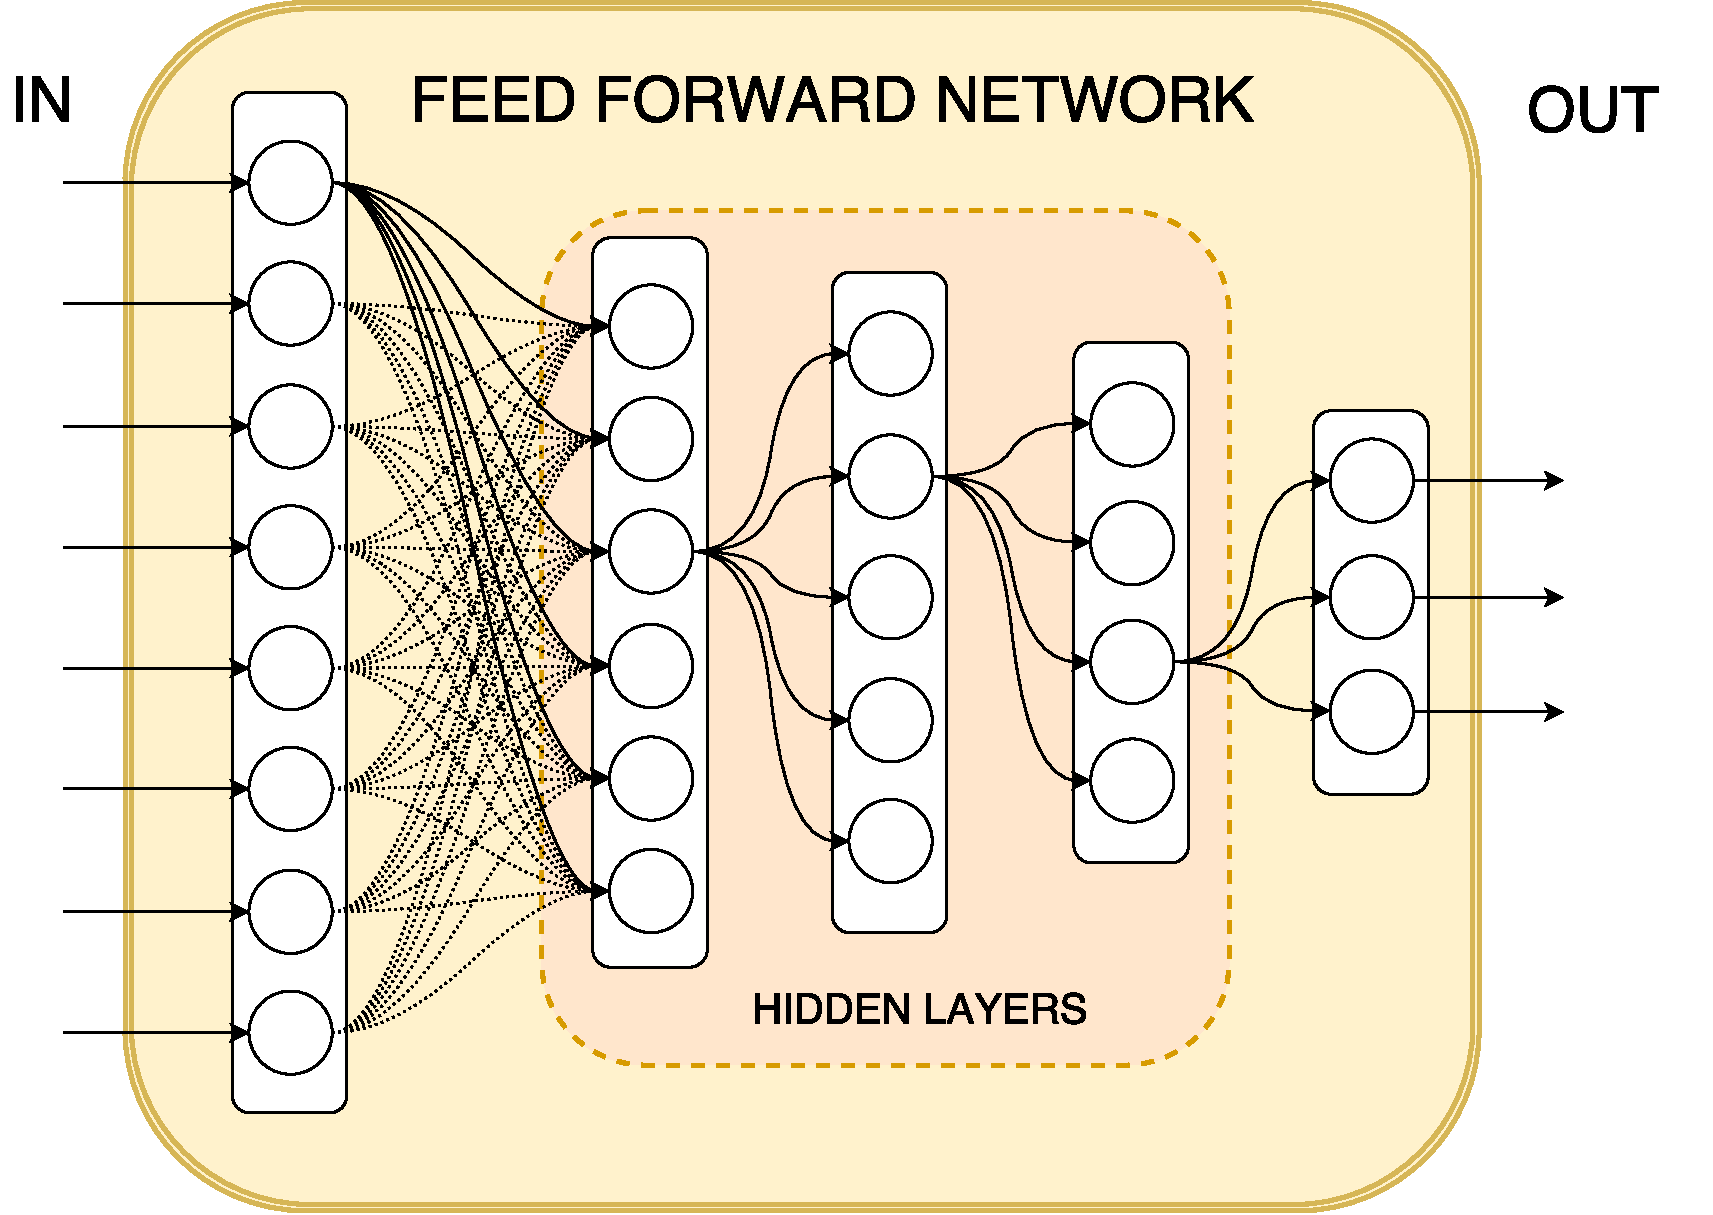
\includegraphics[width=0.6\textwidth]{smallnetwork.pdf}
	\caption{A small feed forward network with three hidden layer composed of Fully Connected layers.
	}
	\label{fig:ff}
\end{figure}

\subsection{Basics of Learning}
After describing the model, the first question is:
\begin{flushright}
    \emph{--- what are the correct values for $\mathbf{w_P}$ for each $   
    \mathbf{P}$ in network $N$?} \\ 
\end{flushright}
There are a lot of intuitive explanations how this problem should be approached and solved. 
For an exhaustive study of the topic, visit Michael Nielsen's website \cite{nnsdl}. 
Anyhow, in general this is still the most studied question in machine learning. 
Luckily, if $N$'s performance can be measured, thanks to its feed-forward structure a \emph{numerical suggestion} can be defined as well, which tells how to change $\mathbf{w_P}$ to improve efficiency of $N$. In practice an $\mathbf{E}$ error function is defined, and the objective of the training is to reduce it. Without digging deep in math we can find an intuitive situation with the same results.\\

Take a perceptron $\mathbf{P}$ with input $\mathbf{x}$ of objects on a given picture of a cat. Suppose that this perceptron \emph{fires} (has high output value) when wheels are on the picture. It should remain silent when there are no round objects listed in 
$\mathbf{x}$, still it turns on, affecting the output of $N$, producing high error.
Since we know the original label of the picture, we can tell which assumptions were wrong, and which were good - which to decrease, which to increase if the next time $N$ is given the same input. 
This information is distributed between the previous perceptrons which caused the current one to fail, by simply multiplying the error with the weight corresponding to the previous node. 
Also with the information of how much the output of the actual node influenced the error, and with its input values, the significance of misleading $\mathbf{x_i}$ can be reduced, and important features' weights can be increased, which is actually finding a better $\mathbf{w_P}$.
For further intuitive examples see section \ref{sec:diff}, or visit Andrej Karpathy's guide \cite{karpathyblog}.

\paragraph{SGD.} The example led to the practical application of the so called \emph{Stochastic Gradient Descent}.
Originally every samples in the training set should be introduced to the system before updating its weights and that would be the \emph{Batch Gradient Descent}, but in  the hope that the samples fall in a subset of the whole space of all possible inputs, the algorithm uses mini-batches for the learning process. When the number of samples in the batches reduces to 1, the training is called on-line training. And if it happens on $N$ containing a single perceptron it is called \emph{Rosenblatt perceptron learning algorithm}.


\section{Inference}
Let us suppose that for a particular task an $\mathcal{F}$ is given, first what we have to understand is how input data 
$x \in \mathbb{X}$ (interchangeably $x_1$) is inferred.
First, assume that the data can be expressed as multi-dimensional matrix, like RGB pictures, audio recordings, gene maps.
Some networks preserve the spatial information i.e. feature extraction performed on images, 
while other instances operate on the whole input data i.e. processing audio samples in frequency domain.
Either way the output $y$ (or $y_L$) can be obtained by feeding $x$ to the network: 
$ y = \mathcal{F}(x)$
The core concept is that we can compose such an $\mathcal{F}$ function by applying multiple projections to $x$.
Practically that means sending input through the first layer, the second, and all the way through to the last layer $L^{th}$, which output would be the value of $\mathcal{F}(x)$, the response of the network.
Therefore in terms of evaluating $\mathcal{F}(x)$ layer by layer, actually translates to a single function call, which can be unfolded to a sequence of embedded projections:
$$
    \mathcal{F}(x) = F_L \left( x_L \right) = F_L \left( y_{(L-1)} \right)
$$
$$
    F_L \left( y_{(L-1)} \right) = 
    F_L \left( F_{(L-1)} \left( x_{(L-1)} \right) \right) = F_L \left( F_{(L-1)}\left( \cdots F_1(x)\right)\right)
$$
Using the function composition operator $\circ$, rewritten in the classical notation:
\begin{equation}\label{eq:forward}
\begin{split}
    \mathcal{F}(x) = F_L \circ F_{(L-1)} \circ \cdots \circ F_1(x)
\end{split}
\end{equation}

The \ref{eq:forward} equation is the most fundamental idea behind feed-forward neural networks, namely the \emph{inference} or \emph{forward-propagation}
As mentioned above, every layer $l$ is represented by an $F_l$. 
The most basic layers are the \emph{Fully Connected} and \emph{Activation} layers.

\subsection{Fully Connected layer} 
These layers carry out the heavy-lifting of inference by performing linear projection and translation transformations. 
The operations are following the rules of basic linear algebra, where the input $x_{FC} \in \mathbb{R}^N$ and the output $y_{FC} \in \mathbb{R}^M$ are specified as real valued vectors.
The parameters of the layer $\phi_{FC}=(W, b)$ are the corresponding weights and biases of each perceptron node in the layer forming a \emph{weight matrix} $W \in \mathbb{R}^{M \times N}$ and a \emph{bias vector} $b \in \mathbb{R}^M$ respectively.
Therefore evaluating the output of the Fully Connected layer is the defined by the following:
\begin{equation}\label{eq:FC}
\begin{split}
    y_i &= \left(\sum_j  W_{i,j} \; x_j \right) + b_i \\
    y &= W \cdot x_j + b \\
    \left[M\right] &= \left[M \times N\right] \cdot \left[N\right] + \left[M\right]
\end{split}
\end{equation}

\subsection{Activation layer} 
Nodes in activation layers are introducing non-linearity to the network, 
by applying the same non-linear activation function to the corresponding output of the previous layer, performing element-wise operation.
Let $F$ be an activation layer with activation function $f$ after a fully connected layer with 3 neurons:
\begin{equation*}
    F(x) = \begin{pmatrix}
    f(x_1) \\ 
    f(x_2) \\
    f(x_3)
    \end{pmatrix}
\end{equation*}
These functions are essential for the network, since they increase the numerical stability: they \emph{squeeze} or \emph{mitigate} the input preventing the network from \emph{saturation} or \emph{explosion} (numerical of course). Conventionally the following functions are applied most often as activation function:
\begin{align}
    \mathrm{Rectified Linear Unit (ReLU) := } &max\left\lbrace 0, x \right\rbrace \label{eq:af1} \\
    \mathrm{Hyperbolic Tangent (TanH) := }   &\tanh(x) = \frac{2}{1+e^{-2x}}-1 \label{eq:af2}\\
    \mathrm{SoftPlus (SP) := }   &\ln(1+e^x) \label{eq:af3}\\
    \mathrm{Logistic (Log) := }  &\frac{1}{1+e^{-x}} \label{eq:af4}
\end{align}
The only constraint on these functions that they have to keep the dimension of the input, namely $F_{act}:\mathbb{R}^N \mapsto \mathbb{R}^N$.
\emph{Note:} These functions do not have any variable parameters, therefore activation layers cannot be trained.

\section{Measuring efficiency}
If the function $\mathcal{F}$ mentioned above is given, and satisfies our needs, then we are done.
However this is usually not the case, and finding the optimal $\mathcal{F}^*$ is the main challenge targeted by many branches of Machine Learning.
Despite it was proven, that standard multilayer
feed-forward networks are capable of approximating
any measurable function to any desired degree of
accuracy \cite{hornik1989multilayer},
if the goal function $\mathcal{F}^*$ is unknown, 
or too abstract to be \emph{measurable} (i.e. telling how funny a picture is), 
we cannot utilize the universal approximator.

\subsection{Loss} 
By reformulating the objective, we can define a Loss function $\mathcal{L}:\mathcal{F}(\mathbb{X}) \mapsto \mathbb{R}$,
which maps our candidate $\mathcal{F}$ network to a scalar field, that represents the general correctness of $\mathcal{F}$ over the space of possible inputs $\mathbb{X}$ -- the lower its value the better $\mathcal{F}$ is performing.
By doing so we may apply Machine Learning algorithms that would \emph{minimize} the Loss, therefore $\mathcal{F}$ would converge towards $\mathcal{F}^*$ implicitly.

\emph{Note:} In practical implementations $\mathcal{F}$ is not evaluated over the whole space of possible inputs, instead in the hope that a small subset of both \emph{training} and \emph{validating} samples called a mini-batch will approximate $\mathcal{L}(\mathcal{F})$ as well. Useful practices for reducing computing complexity and improving stability, and rate of convergence will be covered later.


\subsection{Supervised learning}
In cases where the parameters of $\mathcal{F}^*$ are not known,
but we know how it would map the input space $\mathbb{X} \mapsto
\mathbb{Y}$, e.g. which character appears on the input image $x$, 
then we  can define a set of previously \emph{labeled} pairs of input - 
solution sample which could be used later on for training, and
evaluating performance of the network.

\subsection{Unsupervised learning}
When no labeled dataset is available, the network still can be used for extraction of hidden structure of the unlabeled samples. Later these instances are used as density estimators, or adapted as feature extractors for larger networks.
\textbf{Generative Networks.} Training such architectures can be done by feeding networks random noise as input and training them to reproduce given samples: $\mathcal{F}:\mathbb{R}^k \mapsto \mathbb{X}$, hence the name \emph{Generative Networks}.

\textbf{Auto-encoder Networks} The other frequently applied paradigm is setting the objective task to compress the input sample into a $h \in \mathbb{R}^k$ hidden representation vector that is able to preserve the key information about the original input, and either by symmetric (Restrictive Boltzmann Machines) or independent (Deep Belief networks) operations decompress the data.

In both cases hyper-parameter $k$ is intuitively the number of unlabeled features in the \emph{latent space} that the network will be able to categorize, i.e. correlation between different color intensities on pictures taken of stained brain samples.


\section{Adjusting parameters}
Generally speaking, applying Machine Learning algorithms boils down to the process of iteratively altering parameters $\phi$ of $\mathcal{F}$ to optimize the Loss.
Once $\mathcal{L}(\mathcal{F})$ is obtained, we can evaluate how changing the parameters would influence it -- evaluate the gradient $\nabla_\phi \mathcal{F}$ of the parameters  with regards to $\mathcal{L}$.

\subsection{Gradient Descent}
Updating $\phi$ by descending on the gradient slope with a small step size $\epsilon$ will decrease $\mathcal{L}$.
Derivation from the general form of Gradient Descent depends on the architecture of the network, 
but there is a main concept for doing so, called Backpropagation described by Werbos \emph{et al.} \cite{werbos1994roots}. 
The exact method which can be applied for Fully Connected networks 
will be explained in detail in section \ref{sec:diff}.

\subsection{Training Policies}
Though theoretically after finite steps of iterations, with Gradient Descent $\mathcal{F}$ may approximate any Borel-measurable function, 
in practice Deep Neural Networks can fall into local-minimum of the parameter-space.
I.e. the network tends to learn the very basic features of the input space, if it is not forced to generalize.
The problem with generalization is that the training set has finite samples and extending it requires human-supervision.
Therefore training networks with many layers requires some advanced techniques for training.
There are multiple way to improve the \emph{convergence rate} and the \emph{stability} of the network.

\paragraph{Batch processing.} There are two radical methods of updating the parameters in the network. 

Theoretically if we wanted to create a perfect network, we would infer all possible samples from $\mathbb{X}$ and the Loss function 
$\mathcal{L}$ would evaluate the network on every solution (in a single iteration, without the network being updated), 
then we would take the mean of the Loss to evaluate the gradient, e.g. 
$$\mathcal{L}^*=\frac{1}{N}\sum_{x \in \mathbb{X}}\mathcal{L}(\mathcal{F}(x))$$
One update on the whole training set is called a \textbf{batch}
This way, if the capacity of $\mathcal{F}$ is large enough, it is possible to train the network to be able to solve every problem.
In a special case when we want to simulate logical circuits with real values instead of Boolean \texttt{true} or \texttt{false},
then we can train a network to act like a logical processing unit - since we are able to map $\forall x \in \mathbb{X} \mapsto y \in \mathbb{Y}$ by 
external evaluation.

The other case is more practical, when the train data is not available at once, but in sequence.
The network is usually updated in \emph{testing} time and that is why it is called \textbf{on-line} training.
The topic is described exhaustively in \cite{onlinelearn}.
In practice the network is trained previously before on-line training (even if a very few sample are available), 
because the responses are not just used for evaluating the Loss function, but taken into account as valid predictions.
Normally there is no opportunity to label freshly acquired samples, 
and this is the main reason that this technique is used mainly in \emph{unsupervised learning} tasks.
However when supervision is available, then the network can be trained in the following manner:
predictions which were correct are put into the training set, 
and the network weights are updated immediately 
to encourage the same response for similar samples.
For experiments with the mentioned method, see section~\ref{sec:voice}.
A frequent application of on-line training is called \emph{Q-learn}, for case studies see \cite{qlearn-case}.

Both methods are powerful for specific tasks, but in practice the solution is between: \textbf{mini-batch} training.
Inferring multiple samples at the same time with the same network not just yields a more stable convergence, 
but is an excellent opportunity to parallelize the process:
Extending by one extra dimension to each stage of the inference (inputs, transient activations, outputs) can be done easily,
also almost every library can take the advantage to perform optimized matrix operations on tensors (at least \emph{NumPy} can).
On the second hand, processing only \emph{some} instead of all of the input samples at once is computationally a better choice.
In real applications it is worth considering $2^k$ mini-batch sizes because of the requirement of memory allocation~\cite{stanfordlectures}.

\paragraph{Advanced First order derivatives.} 
Simple heuristics applied to first order derivatives, such as:

\begin{description}[align=right,labelwidth=3cm]
\item[Momentum] \cite{sutskever2013importance}
    $v_{(n+1)}=\gamma v_{n} + \nabla_{\phi_n}\mathcal{L}$ and 
    $\phi_{(n+1)} = \phi_n -\epsilon v_n$
\item[Adagrad] \cite{duchi2011adaptive}
    $r_{(n+1)}=r_n+\left(\nabla_{\phi_n}\mathcal{L}\right)^2$  and 
    $\phi_{(n+1)} = \phi_n - \frac{\epsilon}{\gamma + \sqrt{r_n}} \left(\nabla_{\phi_n}\mathcal{L}\right)^2$ (element-wise) 
\item[RMSProp] \cite{rmsprop} $r_{(n+1)}=(1-\epsilon)r_n + \epsilon\left(\nabla_{\phi_n}\mathcal{L}\right)^2$
\item[Adam] \cite{kingma2014adam} Combination of RMSProp and momentum.
\end{description}
A more sophisticated, but expensive method is using second order derivative, for instance Conjugate gradient \cite{shewchuk1994introduction}.

\paragraph{Decreasing the learning rate $\epsilon$.}
For large networks it is inevitable to use decreasing learning rate, otherwise the convergence would take too much time (small $\epsilon$) or would not even occur (large $\epsilon$). 

\paragraph{Cross-Validation.} Special $\hat{\mathcal{L}}=(\mathcal{L}_{train}, \mathcal{L}_{validation})$ functions approximate the efficiency of the network not just by evaluating them on the currently or previously trained samples, but on samples which are from a totally \textbf{disjunct set} $\mathbb{X}_{validation}$.
The motivation behind it is to see how well would the network perform on samples which it has not faced before.
By doing so we can evaluate how well the network \emph{generalized} the information from samples of the training set.
In order to keep $\mathbb{X}_{train} \bigcap \mathbb{X}_{validation} = \varnothing$ we may not use $\mathcal{L}_{validation}$ for parameter updating.
However in order to \textbf{prevent overfitting} we can monitor e.g. generalization error $E_g=\frac{\hat{\mathcal{L}}_1}{\hat{\mathcal{L}}_2}$ during training 
and use \textbf{Early Stopping} when $E_g > \delta$, where $\delta$ is a parameter of how much we tolerate overfitting.

\subsection{Networks in practice} 
Though networks can vary in shape and function, the representation of the succeeding layers, evaluated by embedded functions described in \ref{eq:forward} is a common feature. Each of these layers serve as nodes of the computational graph of the network. The type of the layer determines whether it can be updated or not: for \emph{Fully Connected} layers $\nabla_\phi F_{FC}$ is well defined, explained in the following example.

\paragraph{Toy example.} 
Assume $\mathcal{L}$ is given, and we have a fully connected network with 2 hidden layers, i.e. $L=3$, which maps a $N$ dimensional input vector $x$ to a $M$ dimensional output vector $y$, namely $\mathcal{F}:\mathbb{R}^N \mapsto \mathbb{R}^M$. The constraint on the parameters are:
\begin{itemize}
    \item[] $W^1$ of the first layer must have $N$ columns
    \item[] $W^3$ and the bias $b^3$ of the last layer must have $M$ rows, dimensions respectively.
    \item[] Number of rows of $W^l$ must match $dim(b^l)$ $3$ dimensional
    \item[] Number of columns of $W^l$ must match $dim(b^{(l-1)})$
\end{itemize} 
Then the evaluation unfolded would look like the following: 
$$y = \mathcal{F}(x) = F_3 \circ F_2 \circ F_1(x) = W^3(W^2(W^1(x)+b^1)+b^2)+b^3$$
For further usage and simplicity, I would like to fix these numbers.
Let $\mathcal{F}$ be a network with the following \emph{shape}: $\left[5, 4, 3\right] $
meaning that in each layer there are 5, 4, 3 neurons respectively, $M=3$ and all nodes are connected to the previous layer. The width of the input layer is not yet defined, let it be $N=10$. 
\emph{Note:} It is usually distracting and redundant to explicitly write the width of the outermost layers when testing different networks, because the input and the output layers must have fixed dimension for the same task, while the width of the hidden layers are varied.
Define an $L_2$ Loss function on the toy example. For one sample-label pair $(x,y^*)$ the $L_2$ Loss is:
\begin{equation}
    \mathcal{L}_2(\mathcal{F}) = \frac{1}{2} \sum_{i} (y_i^* - \mathcal{F}(x)_i)^2 = \frac{1}{2} \sum_{i} (y_i^* - y_i)^2
\end{equation}
$L_2$ is a universal Loss function, which is used in cases where the label space $\mathbb{Y}$ is continuous (e.g. floorspace, consumption and height of a house, based on the price: $\mathbb{R}^1 \mapsto \mathbb{R}^3$).

\section{Differentiation}\label{sec:diff}
In the above evaluating of $\nabla_\phi \mathcal{F}$ can be done in two ways, namely by numerical approximation, or by analytical derivation, in the following I will discuss both.

\subsection{Numeric differentiation} Evaluating the numerical gradient (or difference) is an elementary, yet powerful operation, in which we would \emph{perturb}, or modify one parameter $\phi$ of our system $\mathcal{F}$ at once.
That is done by first adding $\phi^+$ and after subtracting $\phi^-$ a little amount $d\phi$ from the original $\phi$ and evaluate $\mathcal{L}^{\pm}=\mathcal{L}(\mathcal{F}_{\phi^{\pm}})$, namely the \emph{Loss} of the system in the modified state, yielding the numerical gradient in the following equation:

\begin{equation} \label{eq:numgrad}
    \frac{d\mathcal{L}(\mathcal{F})}{d\phi} = 
    \frac{\mathcal{L}^+ - \mathcal{L}^-}{2 d\phi} = 
    \frac{\mathcal{L}(\mathcal{F}_{\phi^+}) - \mathcal{L}(\mathcal{F}_{\phi^-})}{2 d\phi}
\end{equation}

\paragraph{Summary.} In a nutshell value of $\frac{d\mathcal{L}(\mathcal{F})}{d\phi}$ tells how changing the parameter $\phi$ by $d\phi$ would change the performance of the network. If it is positive then updating $\mathcal{F}$ by adding $d\phi$ to $\phi$ would result in higher Loss value, which is the opposite of our goal, so we just subtract it, if it is negative, then trivially we should add $d\phi$ to $\phi$ since it is making some good progress.

\subsection{Complexity} 
Though letting the computer do the hard work seems to be a good idea, it is worth considering that the simple method above will be applied to every $\phi$ of $\mathcal{L}$.
It means that for the network in the toy example, we need to evaluate $\mathcal{L}(\mathcal{F})$ two times for each parameter in 
the weight matrices and the bias vectors of the network, totaling in 
$$\#(\phi) = 2\times\sum_{i=1}^3 N_{(i-1)}\cdot N_i + N_i = 2\times(10\cdot 5 + 5 ... + 4\cdot 3 + 3) = 188$$
Even if $\mathcal{F}$ is approximated by using $k$-sized mini-batches for evaluation it is still a computationally very expensive function, because the inference would result in the following number of operations of addition and multiplication:
$$\#(\mathrm{operations}) = k\times\sum_{i=1}^3 2\cdot N_{(i-1)}\cdot N_i + N_i = k \times 176$$
Therefore approximated with $k=10$ mini-batches would a single parameter update of a very tiny network would require total operations of:
\begin{equation}
    \#(\mathrm{total})=\#(\phi) \times k \times \#(\mathrm{operations}) = 188 \cdot 10 \cdot 176  = 330880
\end{equation}
Because both $\#(\phi)$ and $\#(\mathrm{operations})$ has complexity of $\mathcal{O}(N^2)$, one update will yield complexity of 
\begin{equation}
    \#(\mathrm{total})=\mathcal{O}(N^4)
\end{equation}
We can see that even for a shallow and relatively small network (industrial AI networks has billions of parameters, and uses much larger batches) described in the toy example the method is really costly.
That encourages us to derive our differentials on paper first, and use \emph{numerical gradient approximation} for checking our solution. Using \emph{Gradient Check} is essential when implementing new architectures, because it is a very efficient tool for debugging in comparison with updating. The method in a few words is about setting an error rate $\epsilon$, and decrease $d\phi$ until the numeric solution does not match the analytic solution with $1-\epsilon$ significance. If the analytic solution is incorrect the cycle will not terminate.

\subsection{Analytic differentiation}
Deriving the update by hand requires basic knowledge in calculus extended to multivariate cases, though since the operations are elementary, in general we must understand only three basic definitions to do so. 
Some formality before starting: we have three independent variables $x$, $y$, $z$ and functions $f$, $g$, $h$. The result of operations performed on variables, i.e. $x+2y$ can be represented by a function $f=x+2y$. 
If the value depends on a variable then it can be written explicitly, passing the variable as \emph{the argument} of the function $f(x,y)=x+2y$. 
For the sake of simplicity assume that the variables are not general objects from an abstract space, they are only real values: $x,y,z\in \mathbb{R}$. However the following description could be extended for the above-mentioned variables as well. For any one-dimensional function $f(x):\mathbb{R}\mapsto\mathbb{R}$ we say that the value represented by the function depends on the variable by the extent of its derivative. The derivative (or differential) of the function can be seen as an ideal case of \ref{eq:numgrad} where the perturbation would approach zero, namely:
\begin{equation}
    \frac{\partial f}{\partial x} = \lim_{dx\rightarrow 0}\frac{df(x)}{dx}= \lim_{dx\rightarrow 0} \frac{f(x+dx)-f(x-dx)}{2dx}
\end{equation}
\paragraph{Multiplication rule.}
Consider a value $x\cdot y \cdot z$ represented by $f(x,y,z)$. $f$ is now depending on three variables, we can define the measure of this dependency on one variable by the formal equation:
\begin{equation*}
\begin{split}
    \frac{\partial f}{\partial x} = \lim_{dx\rightarrow 0} \frac{f(x+dx,y,z)-f(x-dx,y,z)}{dx}
    &= \lim_{dx\rightarrow 0} \frac{((x+dx)\cdot y \cdot z)-((x-dx)\cdot y \cdot z)}{2dx} \\
    = \lim_{dx\rightarrow 0} \frac{(x+dx)-(x-dx)}{2dx} y z&= \lim_{dx\rightarrow 0} \frac{2dx}{2dx} yz= yz
\end{split}
\end{equation*}
We can apply the same method for each variable, the result will be the elements of the \emph{gradient} $\nabla f$
\begin{equation}\label{eq:multiplication}
    \frac{\partial f}{\partial x} = y z \qquad
    \frac{\partial f}{\partial y} = x z \qquad
    \frac{\partial f}{\partial z} = x y 
\end{equation} 
The important thing to understand that in a computational graph, a multiplicative node, which takes $N$ arbitrary parameters (or arguments), will have a \emph{partial derivative} for each variable its output is depending on. In general if these derivatives are represented as a vector, then it is called the gradient $\nabla f$ of $f$. Also the value of the derivative will be the product of all variables except the one of which we are computing the influence of on the output.

\paragraph{Addition rule.}
Consider a value $x\cdot y + x\cdot z$ represented by $g(x,y,z)$.
The change of $g$ with respect to $x$ is defined with the following shortened equation:
\begin{equation}\label{eq:addition}
    \frac{\partial g}{\partial x} = \lim_{dx\rightarrow 0} \frac{((x+dx)y +(x+dx)z)-((x-dx)y +(x-dx)z)}{dx}=y+z
\end{equation}
Notice that -- in the terms of computational graphs -- if a node contributes to other different operations (namely $x\cdot y$ and $x\cdot z$), 
than the derivative of each occurrence in \emph{later} values will be summed up. 

\paragraph{Chain rule.}
Let $f(x)=2x+3$ and $g(f)=5f$. Suppose that we would like to know the derivative of $g$ with respect to $x$.
At first we cannot do so, but there are two options: in the hope that substituting the value represented by $f$ into $g$ would not make the equation too complex we can unroll the references and rewrite $g(x)=5\cdot(2x + 3)$, or we could use the chain rule:
$$
    \frac{\partial g}{\partial x} = \lim_{dx \rightarrow 0} \frac{g(f(x+dx)) - g(f(x-dx))}{2dx}
$$

\begin{center}
    Assume that $f(x+dx)-f(x-dx) \neq 0$.
\end{center}

$$
    \lim_{dx \rightarrow 0} \frac{g(f(x+dx)) - g(f(x-dx) ) }{f(x+dx)-f(x-dx)} \cdot \frac{f(x+dx)-f(x-dx)}{2dx}
$$

\begin{equation}\label{eq:chain}
    \frac{\partial g}{\partial x} = \frac{\partial g}{\partial f} \cdot \frac{\partial f}{\partial x}
\end{equation}

Which is a formula of the products of partial derivative of $g$, that treats $f$ like a variable, and $f$ explicitly operating on variable $x$.
The derivative of $g$ with respect to variable $x$ is the product of the \emph{local derivative} of $g$ is $\frac{\partial g}{\partial f}=5$ and $\frac{\partial f}{\partial x}=2$ which equals $\frac{\partial g(x)}{\partial x}=\frac{\partial(5\cdot (2x + 3))}{\partial x} = 10$, the function strictly depending on $x$.
The important message is that we can interchangeably use function values and variables with a constraint that at a point, in an arbitrary depth there must be a real variable.
\emph{Note:} the statement above stands for computations with \emph{Acyclic Graph}, meaning that there should not be any feedbacks or loops -- no definitions like $f(g), g(f)$ or $f(f)$.
We will see that these rules play a very fundamental role in training networks.

\paragraph{Vector Notation.}
Before drilling deep into mathematical equations, a small reminder: the following vector and matrix formulation is just a special annotation, 
using the rules above, which helps to make clear both the definition, and the computations done by the network when it is implemented. 
The vectors with partially derivatives inside are just representing \emph{real values}, arranged in a fancy way.
Every vector and matrix defined in forward propagation, has its corresponding derivative w.r.t. the Loss.
More trivially, if any value is depending on a list of variables $f(x_1, x_2 \cdots x_n) = f(\mathbf{x})$ (a vector) then there is a list of \emph{partial derivatives} w.r.t. to $f$ -- forming the gradient $\nabla f = \left(\frac{\partial f}{x_1}, \frac{\partial f}{x_1} \cdots \frac{\partial f}{x_N}\right)$. 
\emph{Notation}: When the vector notation is emphasized the variable name is conventionally written in bold font $\mathbf{x}$, or is underlined \underline{$x$}.
Because later the indexing would become too crowded, we only use the indexed notation when it is necessary, otherwise using $x$.

The next step is formulating the dependency of multiple functions on multiple variables.
As seen above, a multivariate function has its gradient vector --
in the same fashion as the list of variables were organized into vectors $\mathbf{x}$, values composed of them can also form a vector $F = (f_1, f_2 \cdots f_M)$, composing a multivalued function depending on the same variables.
Doing so yields a first-order derivative matrix, composed of gradient vectors $J=(\nabla f_1, \nabla f_2 \cdots \nabla f_M)^T$, called the \emph{Jacobian of $F$}.
The Jacobian has as many rows as output values $F$ has, and the same number of columns of the variables that $f_i$ is a function of.
\begin{equation}\label{eq:jacobian}
    J(F) = 
    \begin{pmatrix}
    \quad \nabla f_1 \quad \\ 
    \vdots \\ 
    \nabla f_M
    \end{pmatrix} 
    =
    \begin{pmatrix}
    \frac{\partial f_1}{\partial x_1} & \cdots & \frac{\partial f_1}{\partial x_N} \\ 
    \vdots & \ddots & \vdots \\ 
    \frac{\partial f_M}{\partial x_1} & \cdots & \frac{\partial f_M}{\partial x_N}
    \end{pmatrix} 
\end{equation}
The matrix and vector operations (such as addition and inner product) that can be performed on the derivative \emph{arrays} are identical defined in the inference section. That is important because product of derivatives introduced by the chain rule, can be applied as well for multidimensional array of derivatives too.

\subsection{Fully Connected Layer}
Return to the toy example and begin with the last layer, with $3$ nodes. If a sample $x$ is inferred $\mathcal{F}(x)=y$, then the response of the network will be a vector of $dim(y) = 3$. If we took the $L_2$ \emph{distance} between the response and the goal $y^*$, then it would tell how far we are from the ideal, by a single scalar value. Since we want to minimize it, we have to adjust the parameters of the network, namely descend on the gradient slope. To get the small extent of the update we have to evaluate $\frac{\partial\mathcal{L}}{\partial \phi}$. 
Intuitively in the case we would like to correct the weights of a decision, it would require two things:
\begin{itemize}
    \item[] The original situation (the input of the $l^{th}$ layer $x_l$), which the decision was made in.
    \item[] The error on the decision -- the derivative $\delta^l$ of the Loss with regards to the decision.
\end{itemize}
Since $x_l$ is obtained via inference, what we have to calculate is $\delta^l$ for the $l^{th}$ layer in order to acquire the parameter gradient.
The first step is to evaluate the $\delta_L$, or the \emph{error} of the last layer's response $y^3$, namely $\delta^3 = \nabla_{y^3} \mathcal{L}$.
Begin with the first element: 
$$
    \delta_1^3 = 
    \frac{\partial \mathcal{L}}{\partial y_1} = 
    \frac{\partial}{\partial y_1}\frac{1}{2}\left((y^*_1 - y_1)^2 + (y^*_2 - y_2)^2 + (y^*_3 - y_3)^2\right) = y_1 - y^*_1
$$
\begin{center}
Expanding it to the whole array:
\end{center}
$$
    \delta^3 = \begin{pmatrix}
     \frac{\partial \mathcal{L}}{\partial y_1}\\ \\
    \frac{\partial \mathcal{L}}{\partial y_2} \\ \\
    \frac{\partial \mathcal{L}}{\partial y_3}
    \end{pmatrix} = \begin{pmatrix}
     \frac{\partial}{\partial y_1} \frac{1}{2}\sum_i(y_i^*-y_i)^2\\ \\
    \frac{\partial}{\partial y_2} \frac{1}{2}\sum_i(y_i^*-y_i)^2 \\ \\
    \frac{\partial}{\partial y^3_3}  \frac{1}{2}\sum_i(y_i^*-y_i)^2
    \end{pmatrix} = \begin{pmatrix}
     {y_1-y^*_1}\\ \\
     {y_2-y^*_2}\\ \\
     {y_3-y^*_3}
    \end{pmatrix} 
$$
Consider the following notation:
$
    \delta^3_i = (y^*_i - y_i)
$, 
called parametric vector notation. Writing arrays in this way, saves a lot of space. However, when this notation gets jammed with indexes, it is useful to write down explicitly the whole array for clarification.

\paragraph{The last layer} Now we have exact values of $\delta^3$ and $x^3$, so we can calculate how should the weights in $W^3$ be changed in order to get a better network.
Applying the differentiation rules for each weight (forming a matrix) of the layer will result in a derivative for each weight (also forming a matrix).
Taking the first perceptron of the layer, it has a weight $W^3_1=(W_{1,1}, W_{1,2}, W_{1,3}, W_{1,4})$ for each output of the previous layer.

Suppose that this neuron had to tell how rounded is the object on an image sample, 
and the $i^{th}$ neuron of the $2^{nd}$ layer fires when it recognizes sharp edges.
Of course it would be bad if our neuron had a large weight on $x^3_i$. 
If this node performs poorly because of $x^3_i$, then it would contribute a lot to the Loss function while inferring sharp objects, with its output $y_1$ being far away from $y^*_1$, resulting in a positive $\delta^3_1$. 
In case of $x^3_i = 0$, the weight $W_{1,i}$ has nothing to do with the error $\delta^3_1$ of the neuron.
Notice that the error of each weight (w.r.t $\mathcal{L}$) should be proportional to the error and the input as well: $\frac{\partial \mathcal{L}}{\partial w_{1,i}}=x^3_i \cdot \delta^3_1$.
However it can be also derived in terms of the differentiation rules: 
$$
    \frac{\partial \mathcal{L}}{\partial W_{1,i}}=
    \frac{\partial \mathcal{L}}{\partial y^3_1}\cdot \frac{\partial y^3_1}{\partial W_{1,i}} =
     \delta^3_1  \cdot x^3_i
$$

\paragraph{Considering the parameter update.} assume that a picture of an origami sculpture (a very edgy one) was inferred and the $i^{th}$ node of the second layer worked correctly. Both $x^3_i$ and $\delta^3_1$ is positive, however the weight should be decreased: that is why we will take the negative of the derivative for updating $w_{1,i}$.
Substituting $i=1,2,3,4$ into $\frac{\partial \mathcal{L}}{\partial w_{1,i}}$ yields a gradient of $\mathcal{L}$ with regards to the weights of the first neuron of the last layer. 
Doing so for each neurons in the layer would result in 3 gradient vectors $\nabla_{W_1} \mathcal{L}$, $\nabla_{W_2} \mathcal{L}$ and $\nabla_{W_3 }\mathcal{L}$ which is practically stacked to make a matrix which can be later added element-wisely to the weight matrix $W$.
$$
\nabla_W \mathcal{L} = 
\begin{pmatrix}
\frac{\partial \mathcal{L}}{\partial W_{1,1}} & \frac{\partial \mathcal{L}}{\partial W_{1,2}} & \frac{\partial \mathcal{L}}{\partial W_{1,3}} & \frac{\partial \mathcal{L}}{\partial W_{1,4}} \\ \\
\frac{\partial \mathcal{L}}{\partial W_{2,1}} & \frac{\partial \mathcal{L}}{\partial W_{2,2}} & \frac{\partial \mathcal{L}}{\partial W_{2,3}} & \frac{\partial \mathcal{L}}{\partial W_{2,4}} \\ \\
\frac{\partial \mathcal{L}}{\partial W_{3,1}} & \frac{\partial \mathcal{L}}{\partial W_{3,2}} & \frac{\partial \mathcal{L}}{\partial W_{3,3}} & \frac{\partial \mathcal{L}}{\partial W_{3,4}}
\end{pmatrix} = 
\begin{pmatrix}
 x_1 \delta_1 &  x_2 \delta_1 &  x_3 \delta_1 &  x_4 \delta_1 \\ \\
 x_1 \delta_2 &  x_2 \delta_2 &  x_3 \delta_2 &  x_4 \delta_2 \\ \\
 x_1 \delta_3 &  x_2 \delta_3 &  x_3 \delta_3 &  x_4 \delta_3
\end{pmatrix}
$$

The last part of the equation can be also expressed as:
\begin{equation}
\nabla_W \mathcal{L} = \left(\frac{\partial \mathcal{L}}{\partial W_{i,j}}\right) = \left(x_j \delta_i\right) = x \wedge \delta
\end{equation}
Where $\wedge$ denotes the \emph{outer product} operator. 
The gradient of the bias is simply $\nabla_{b^L} \mathcal{L} = \delta^L$.

\paragraph{The $(L-1)^{th}$ layer.} Gradient descent can be applied on networks with more than one layer, 
however continuing the example of the image descriptor network requires a bit more abstraction. 
In the previous explanation we assumed that the $i^{th}$ neuron of the second layer worked properly.
In general cases this assumption is incorrect, if the whole network is initialized at once.
If we think about that also the mentioned neuron in the \emph{last hidden layer} should be trained, 
then we can apply the same method with a 4 dimensional $\delta^{(L-1)}$ and with a 5 dimensional $x^{(L-1)}$ input.

\emph{Note}: Capital $L$ is representing the number of layers. In the toy example $L = 3$.\\
Acquiring the $\delta^{(L-1)}$ is where the chain rule \eqref{eq:chain} steps into the scene.
While in the example before we could find an intuitive workaround, in this case it would be quite strained, since $\mathcal{L}$ does not depend directly on $y_{(L-1)}$.
Utilizing the chain rule:
\begin{equation}\label{eq:backward}
    \delta^{(L-1)} = 
    \frac{\partial \mathcal{L}}{\partial y^{(L-1)}} = 
    \frac{\partial \mathcal{L}}{\partial y^{L}} \cdot
    \frac{\partial y^{L}}{\partial y^{(L-1)}} = 
    \delta^L \cdot J(F_L)
\end{equation}
Where $J(F_L)$ denotes the \emph{Jacobian} \eqref{eq:jacobian} of the function representing the projection of the last layer $F_L:\mathbb{R}^4\mapsto \mathbb{R}^3$.
It is a map of how each input variable affects the output of the layer.
In general: the Jacobian numerically can be represented as a $3 \times 4$ matrix, analytically as a \emph{local derivative} of function $F$.
In case of \emph{Fully Connected} layers the Jacobian is simply the weight matrix $F(F_l)=W_l$ (the bias drops out here).

For derivative of scalar values ($\mathbb{R}$) the \emph{product} operator is well defined, 
and it can be expanded the same way to derivatives of multidimensional values as 
regular \emph{inner product} of the values they are composed of.
\emph{Note}: In order to stay consistent with the dimensions of the computation, we have to switch sides of the matrix multiplication defined in \eqref{eq:FC}:
\begin{equation}\label{eq:reverse}
\begin{split}
\delta^{(L-1)}_j &= 
    \sum_j \delta^L_i \; W^L_{i,j} \\
    \delta^{(L-1)} &= \delta^L \cdot W^L\\
    \left[4\right] &= \left[3\right] \cdot \left[3 \times 4\right] 
\end{split}
\end{equation}
\subsection{Backpropagation}
The backpropagation algorithm, first described by Werbos \emph{et. al} \cite{werbos1994roots}
\paragraph{The $l^{th}$ layer.} 
The contribution to the Loss of the general $l^{th}$ layer $\delta^l$ can be retrieved by unfolding $\frac{\partial \mathcal{L}}{\partial y^l}$ applying the chain rule, namely the backpropagation:
\begin{equation}\label{backprop}
\begin{split}
    \delta^l &= 
    \frac{\partial \mathcal{L}}{\partial y^{l}} = 
    \frac{\partial \mathcal{L}}{\partial y^{L}} \cdot
    \frac{\partial y^{L}}{\partial y^{(L-1)}} \quad \cdots \quad
    \frac{\partial y^{(l+1)}}{\partial y^{l}} \\
    \delta^l &= \delta^L \cdot J(F_L) \cdot J(F_{(L-1)}) \quad \cdots \quad J(F_{(l-1)})\\
    \left[dim(l)\right] &= \left[dim(L)\right] \cdot \left[dim(L)\times dim(L-1)\right] \cdots \left[dim(l+1)\times dim(l)\right]
\end{split}   
\end{equation}
\emph{Note}: the order of evaluating these derivatives is theoretically irrelevant, 
however computationally there is an opportunity to implement it in two ways \cite{akthesis}:
\begin{enumerate}
    \item[] \emph{forward-mode differentiation}: evaluating in the order of layers is efficient in cases where the output of the network is much larger than the input
    \item[] \emph{reverse-mode differentiation}: evaluating in reversed order for networks with fewer outputs than inputs.
\end{enumerate}
As pointed out in the thesis, the former would require $(L-l)$  times evaluating a \emph{matrix-matrix} product and one \emph{vector-matrix} operation,
while the latter would require $(L-l)$ times evaluating a \emph{vector-matrix} product and one \emph{matrix-matrix} at the end. 
Using forward-mode differentiation does not require keeping transient activations $y^l$, however it is computationally costly.
Using backward-mode differentiation does not strain the CPU, but the memory. 
It is because if $J(F_l)$ is not linear, then it requires the input $x_l$ to evaluate the first order derivatives.

\subsection{Activation Layer} 
Though the activation layer operates on the input, it has no adjustable parameter. 
Since we have to evaluate $\delta$ for layers behind activation layers, the error must pass through $J(F_{activation}$ as well.
Luckily activation layers applies a scalar function element-wise on the inputs, 
the Jacobian of the composite function $F$ has a special attribute: it is \textbf{diagonal}, meaning that:
$$
    J(F) = \frac{\partial F_i}{\partial x_j} = 
    \begin{cases}
        \frac{\partial f(x_i)}{\partial x_i} & i = j\\
        0 & i \neq j
    \end{cases}
$$
We can exploit this function when implementing activation layers, by simply using element-wise product $\frac{\partial f(x_i)}{\partial x_i}$ instead of a matrix multiplication.
The mentioned activation functions (\ref{eq:af1}, \ref{eq:af2}, \ref{eq:af3}, \ref{eq:af4}), are differentiable \emph{almost everywhere}, the corresponding derivatives:
\begin{align}
    \mathrm{(ReLU)' := } &\mathrm{Heaviside}(x)\\
    \mathrm{(TanH)' := }   & 1 - \tanh(x)^2\\
    \mathrm{(SP)' := }   &\frac{1}{1+e^{-x}}\\
    \mathrm{(Log)' := }  &\mathrm{Logistic}(x)\cdot (1-\mathrm{Logistic}(x))
\end{align}


\section{Implementation}
As I have mentioned in the beginning of the chapter, before implementing my own library I have analyzed multiple source-codes and tutorials. 
Practical considerations led me to the current concept of neural networks, which will be described in this section.
I will also introduce special layers derived from the abstract layers, 
with the common attribute: the lack of trainable parameters. 
Some of these layers are only used for manipulating the shape of information flow, 
while others are down-sampling the input signal, 
and there are layers which are removed from the network after training.


\subsection{Layers as building blocks}
Taking into account the functions of a general layer, 
I made an abstract object with interface to implement
by derived layers. 
The most important attributes of the \url{abstract_layer}:
\begin{itemize}
\item[] \url{get_local_output} performs the \emph{forward-pass} of the layer on its argument
\item[] \url{backprop_delta} performs the \emph{backward-pass} of the layer for a given delta
\item[] \url{prev} and \url{next} fields pointing to other layers
\item[] \url{get_output} and \url{get_delta} uses \url{prev} and \url{next} to unfold the \ref{eq:forward} and \ref{eq:backward} function calls.
\end{itemize}

\subsection{Network as layer manager}
In my implementation the \texttt{network} is an object that arranges, connects, train and utilize layers.
While layers can function without a network, for ease of use and modularity purposes
the network takes care of managing the computational graph.
The use of \texttt{network} class enables to implement high-level features such as:
defining training policies, serializing saving and loading networks on hard drive,
visualizing layers.
The network can add existing layers to its graph, and also makes it easier to create new ones and remove others.
Below the definition and the train of the network which performs over 98\% on MNIST.
\clearpage
\begin{lstlisting}[language=Python]
import network_module as nm
...
# train is a two element tuple consisting of:
#   50k MNIST image 
#   their corresponding one-hot labels.

# initialize network with 784 wide input layer and SoftMax loss function
nn = nm.network(in_shape=np.prod(train[0][0].shape), criterion='softmax') 

nn.add_full(784) # add fully connected layer of 784 neurons
nn.add_activation('relu') # add layer with ReLU activation function

nn.add_full(784)
nn.add_activation('relu')

nn.add_full(100)
nn.add_activation('tanh')

nn.add_full(10) 

# the last layer always determine the shape of the output
# the network updates its output layer automatically when a layer is added

# train the network with the given parameters
nn.SGD(train_policy=nn.fix_epoch, epoch=25, training_set=train,
       batch=128, rate=0.05, L2=True, reg=0.001)
\end{lstlisting}



\subsection{Shaper} This layer does not manipulate the values of its input, but as the name suggests, it rearranges the values and also redirects the gradient flow.
Its activation function $f(x) = x$ is the identity function, and its derivative is also quite straightforward $f(x)'=1$.
Used for networks, where a single input is not one dimensional and has to be \texttt{flatten} before inference, or in \emph{multi-thread} networks where the inference is distributed between parallel layers \cite{szegedy2015going}.
\paragraph{Input.} In my implementation, for practical considerations I use the \texttt{input} layer, the $0^{th}$ layer, for reshaping the input samples (if required).

\subsection{Pooling layers} Pooling layers are decreasing the parameter space with a fixed down-sampling projection which operates independently on tiles of input.
In general pooling layers are moving a \texttt{N}-sized window, or a tile through the data taking \texttt{stride} steps.
Data in each window is collapsed by an aggregation function, such as \texttt{mean()} or \texttt{max()} lowering the computational complexity of the next layers processes. Implementation of this layer can be a bottleneck of inference, since the operations carried out in each window may rely on the same input values if \texttt{N} $>$ \texttt{stride} i.e. windows overlap. In my library a single \texttt{max-pool} layer is implemented with fixed parameters: \texttt{stride} $=$ \texttt{N} $=2$. Further information see~\cite{stanfordlectures}~\url{~/convolutional-networks/#pool}.

\subsection{k-WTA}
\emph{k-Winner Takes All} layers are similar to pooling layers, without preserving spatial information.
They function as a threshold of the previous layer, only passing those activations which have the largest magnitude among the others. 
Gradient is also distributed between those neurons which were passed by the \emph{k-WTA} layer.
Mainly used in fully-connected networks for reducing computational complexity.
This layer was applied when generating MNIST visualization.
For further information see~\cite{wta}.

\subsection{Dropout} Dropout layers target the problem of overfitting, being considered as a method of regularization.
In theory they reduce complex co-adaptation via model averaging, 
by generating different networks (using the same parameters) in each forward pass~\cite{hinton2012improving}.
Practically they drop activations of the previous layer (with random \emph{Bernoulli($p$)} probability) when propagating information, forcing succeeding layers to not depend on an individual neuron of the layer before.  
Computationally it is very efficient to create different, so called \textbf{sub-networks}: both for forward and backward pass a single \emph{Boolean array} mask is used.
\emph{Note}: Dropout layers are reducing the overall magnitude of the activation of the previous layer,
considering that latent layers would be \emph{saturated} when dropout layers were removed after training,
the activations passed by this layer are multiplied by the constant $\frac{1}{p}$.
\paragraph{DropConnect} A similar concept, introduced by Li Wan \emph{et al.}~\cite{dropcon}: 
instead dropping the activation of the previous layer, the weights of the layer are canceled out in the same fashion.
In my implementation they can be only applied to fully-connected layers, where a \emph{Boolean matrix} mask is used.

\subsection{Output} 
On the top of every network there should be a dedicated layer, which arranges the networks response. 
If a \emph{(sample, label)} pair was inferred it also evaluates the result and output a \emph{(response, loss)} pair.
Therefore the output layer will determine how the network will be trained, and the response interpreted
\paragraph{Softmax.} In case of classification, 
when the network has to decide which set was the input sampled from, 
then we can transform the response into a categorical probability distribution, 
i.e. how confident each neuron in the last layer in classifying the input as their 'own'.
For that, we use \textbf{one-hot} notation, where $y^*_i = \left[ 0,0 \cdots 1 \cdots 0\right]$ (with only one non-zero element) represents the \emph{ground-truth} label, the $i^{th}$ class.
The response will be turned into a discrete density function, e. g. $  = [0.1, \; 0.6, \; 0.2, \; 0.1]$ can be interpreted as the following:
the input $x$ is categorized as a sample from the second class with 60\% confidence. Notice that $|p|_1=\sum_i y_i=1$ constraint should be satisfied.
To transform a real valued $N$ dimensional vector $y \in \mathbb{R}^N$ to the mentioned probability distribution $p\in \Omega^N$ we apply the \emph{Softmax} function:
\begin{equation}
p_i = \frac{\exp(y_i)}{|\exp(y)|_1}
\end{equation}
Conventionally the corresponding Loss function is the \textbf{log-loss} or \textbf{cross-entropy} function:
\begin{equation}
\mathcal{L}(y)=-\sum_i y^*_i \log p_i
\end{equation}
and the derivation of its gradient w.r.t. the original response of the last layer $y$, is the following (based on \cite{softmax}):
\begin{equation}\label{eq:softmax}
\begin{split}
\frac{\partial \mathcal{L}}{\partial y_i} &=
-\sum_k y^*_j \frac{\partial \log p_j}{\partial y_i} = 
-\sum_k \frac{y^*_j}{p_j}\frac{\partial p_j}{\partial y_i} \\
&= -y^*_i\left(1-p_i\right) - \sum_{j \neq i} \frac{y^*_j}{p_j}\left(p_i p_j\right) \\
&= -y^*_i-y^*_i p_i + \sum_{j \neq i} y^*_j p_i \\
&= -y^*_i + \sum_j y^*_j p_i \\
&= p_i \left(\sum_j y^*_j\right) -y^*_i \\
&= p_i - y^*_i
\end{split}
\end{equation}
The trick of the derivation is that $y^*$ has only one non-zero element which is 1, and the lemma:
$$
\frac{\partial p_j}{\partial y_i} = 
\begin{cases}
    p_i(1-p_i) & i=j \\
    -p_i p_j & i \neq j
\end{cases}
$$
	%
\clearpage
\chapter{Case studies and Results}\label{cp:results}

\section{Voice recognition}\label{sec:voice}

Today's neural networks work on algorithmically very complex, yet 
intuitive tasks. These objectives can be categorized into two main 
classes: \emph{supervised} and \emph{unsupervised}. 
The trend shows that sample labeling slavery becomes unfavored, 
because human-resource for classifying and evaluating tasks is getting more expensive.
Therefore classical supervised learning is getting less attention over time. 
Still understanding how these models (should) work is essential and 
demonstrating via the simplest examples leads to some interesting case 
studies. In the following an informal introduction presents results of 
such experiments.

\paragraph{Technical background.} 
For the sake of readability the detailed implementation of the perceptron 
framework is excluded from this work (although can be found in 
\url{~/tree/master/demo/audio} at the GitHub repository of my implementation \cite{DV}). 
The writing assumes basic knowledge in linear algebra, the model will be described in the following manner:
 
\begin{figure}
	\centering
	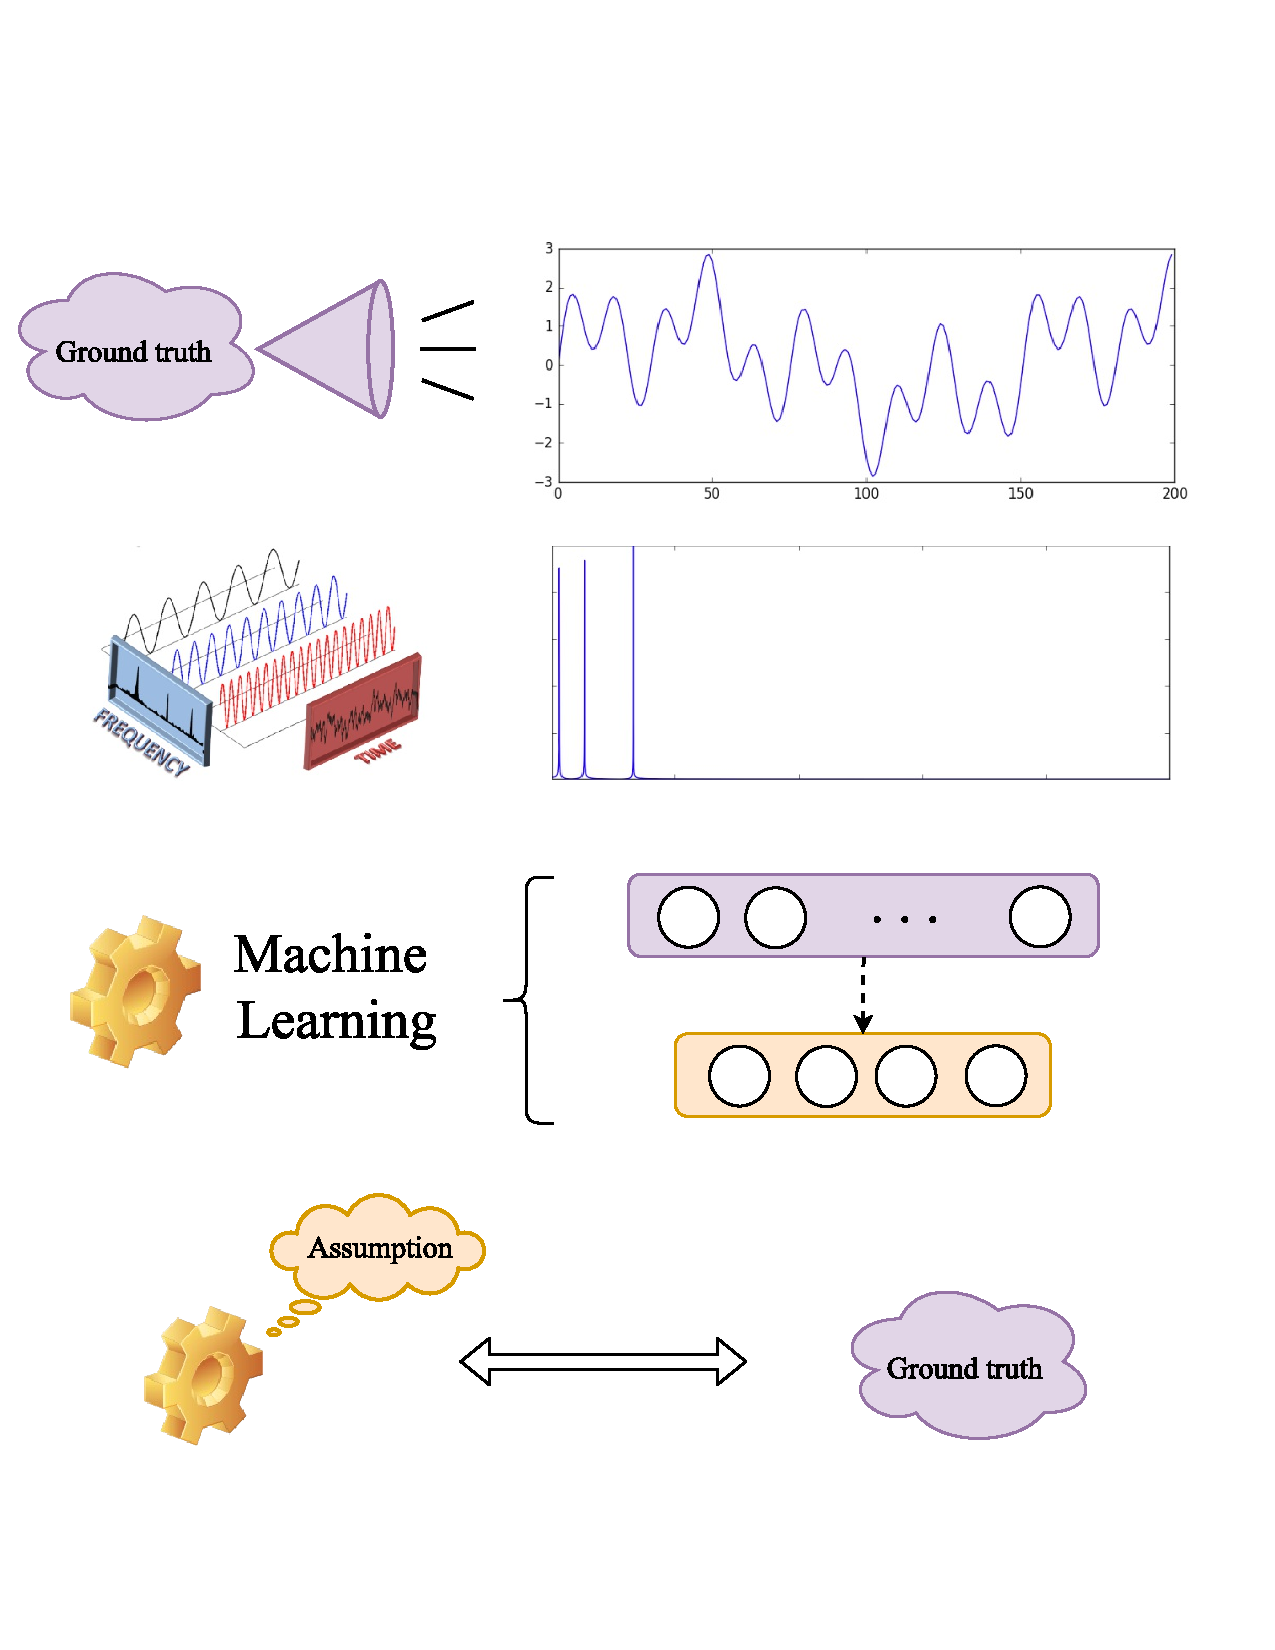
\includegraphics[width=0.9\textwidth]{workflow.pdf}
	\caption{
	The basic conception of voice recognition: 
	the original message is first expressed in physical waveforms which may introduce a lot of noise in real life. 
	After recording, the wave in time domain, it is transferred to \emph{frequency domain} that 
	tells which frequencies were dominant in the captured signal sample.
	According to nature's biological systems in this form the same information can be better processed.
	}
	\label{fig:workflow}
\end{figure}
For a given network $N$ and fixed length input $x$ the system's assumption, the output, is computed as $y=N(x)$, where $y$ is a fixed length vector.
$N$ can be seen as a \emph{black box}, that takes $dim(x)$ information, somehow processes it and - if $N$ is trained correctly it returns the class of $x$. Practically $dim(y)=|\{\textrm{classes}\}|$ - therefore $y$ represents the network's confidence on each class.

\subsection{Separating sine waves}
After defining the model, the first implementation should be able to classify the low- and high-pitch samples. For starting let the low-pitch sample, $\mathbf{x^1}$ be a sine function with frequency $F1$, and high-frequency sample $\mathbf{x^2}$ a sine with frequency $F2$. 
For mimicking the nature's living systems (especially the inner ear), the sample is transformed to frequency domain with an algorithm called \emph{N-point Fast Fourier Transform} \cite{welch1967use}. 
\paragraph{Fourier Transform in a nutshell.} Basically the result of the transformation tells which frequencies were dominant in the time domain, which is a better clue for both the living, and the machines too. 
The architecture will be two perceptrons in the same layer. 
For each $\mathbf{x_i}$ they have different weights, which helps them decide when to turn on, and when to output lower value. 
For details see Figure \ref{fig:N500}. 
For the script which was used to produce the figures check out \cite{DV}.

\begin{figure}
	\centering
	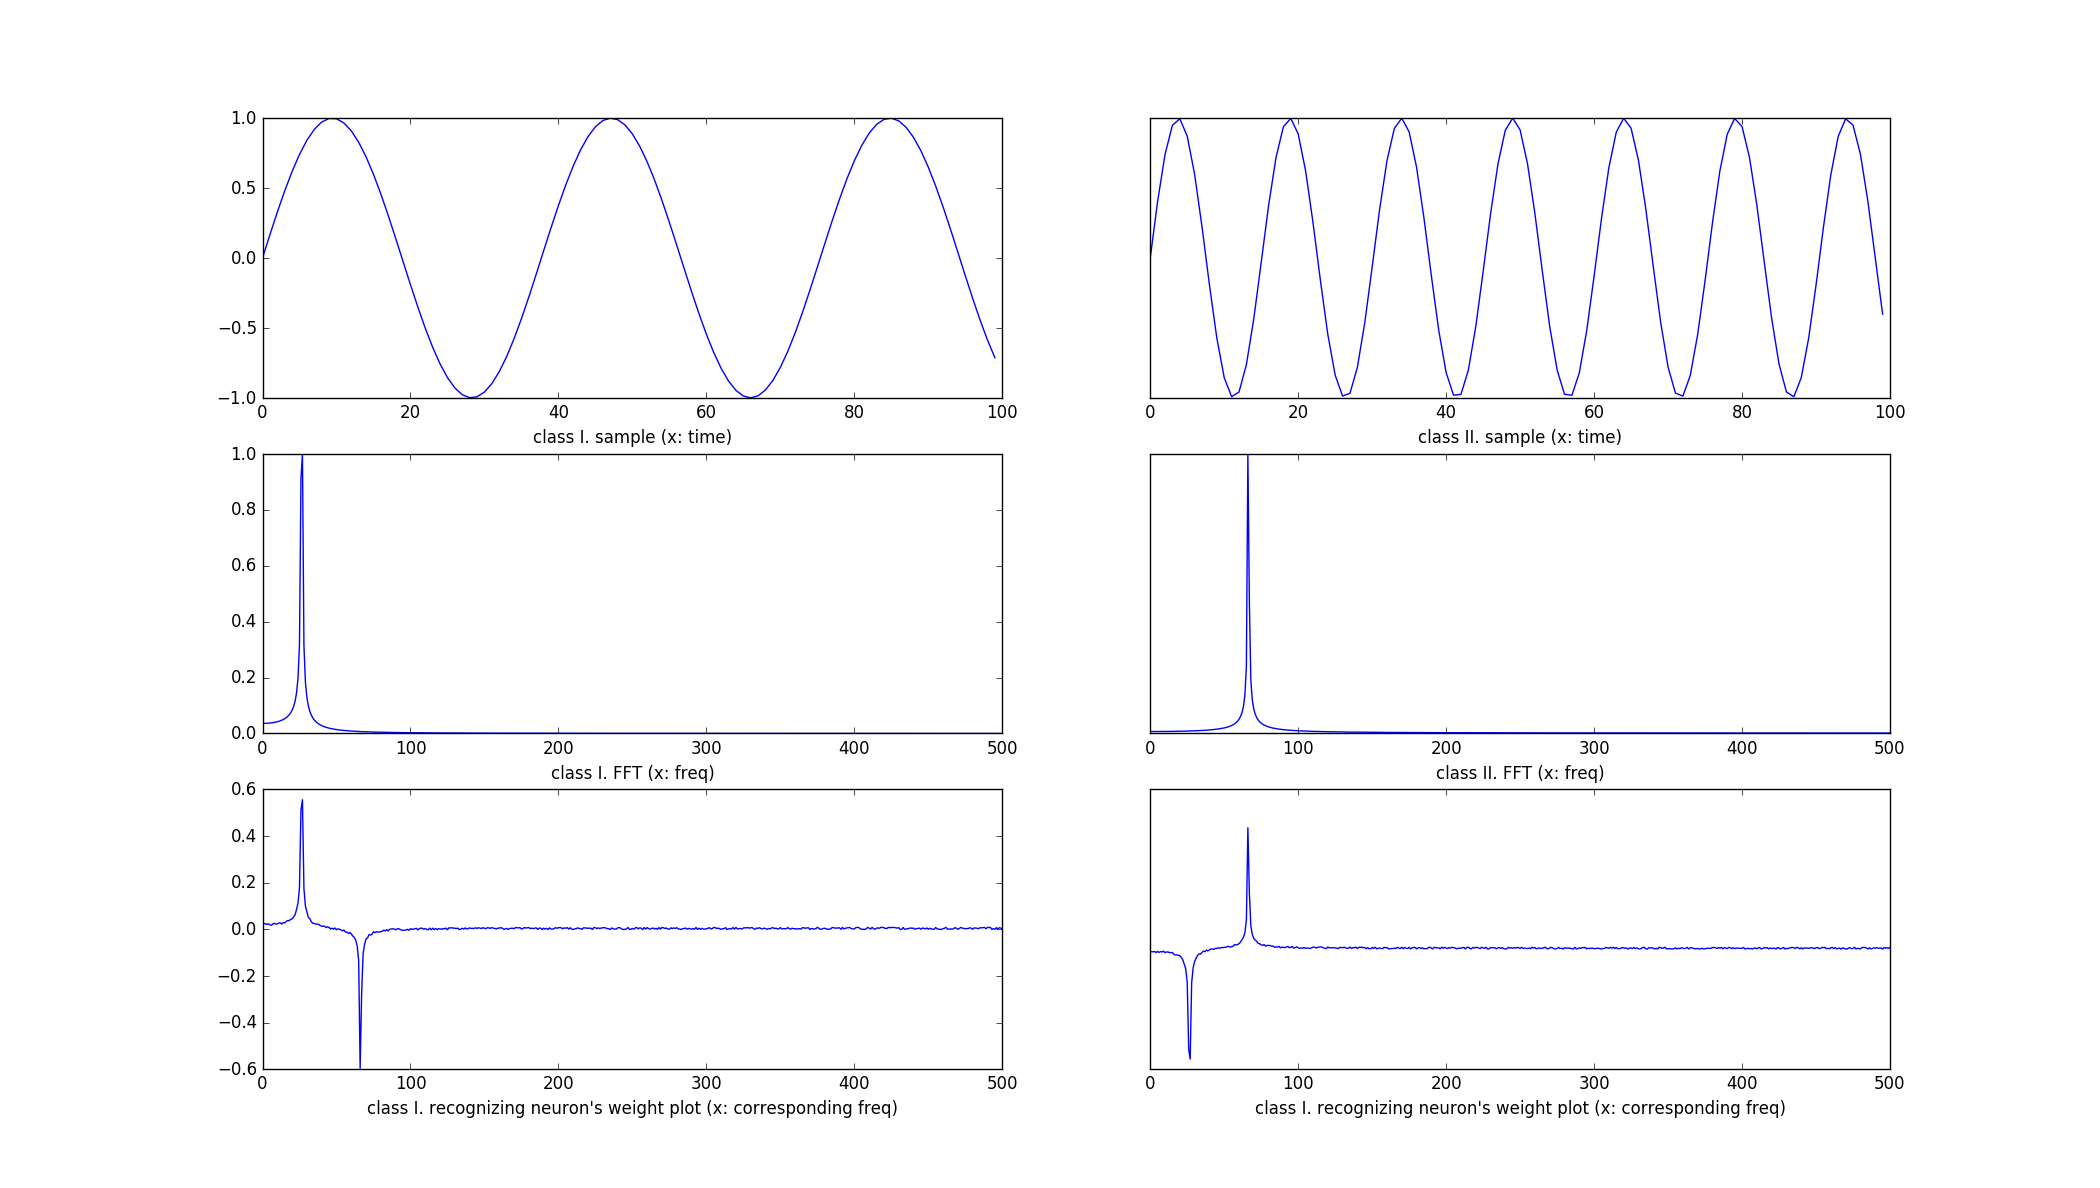
\includegraphics[width=0.8\textwidth]{N500-L2e-1.png}
	\caption{On the first row the original sample is shown in time domain.
	 On the second row the N-FFT of it. On the last row the plot of the 
	 weights of the corresponding perceptron. 
	 The first feature to 
	 recognize, that each perceptron learned that not just to turn on for 
	 the corresponding input sample, but to output negative values when 
	 samples of the opposite class are shown to the network. 
	 The network 
	 was initialized with Gaussian random noise with mean at 0 and 
	 deviation $1/2$, and trained with mini-batch size 1, learning rate $
	 \eta=0.5$, \emph{regularization} factor $\lambda=0.1$ for 10 epoch 
	 with \emph{cross-likelihood} error function}
	
	\label{fig:N500}
\end{figure}

\paragraph{Varying the precision of the Fourier Transform, N.}
For such arbitrary cases, where no noise is added to the signal, larger precision is unnecessary, for validation check Figure \ref{fig:N5000}, \ref{fig:N50}. However the importance of choosing the right N should not be underestimated: in environments with loss \emph{Signal-to-Noise ratio} it is advised to use high \emph{sampling rate}, and large $N$, however for real-time applications it is a trade-off between quality and speed, because the computation complexity for this architecture is $\mathcal{O}(N^2)$, therefore choosing too large N results in slow processing.

\begin{figure}
	\centering
	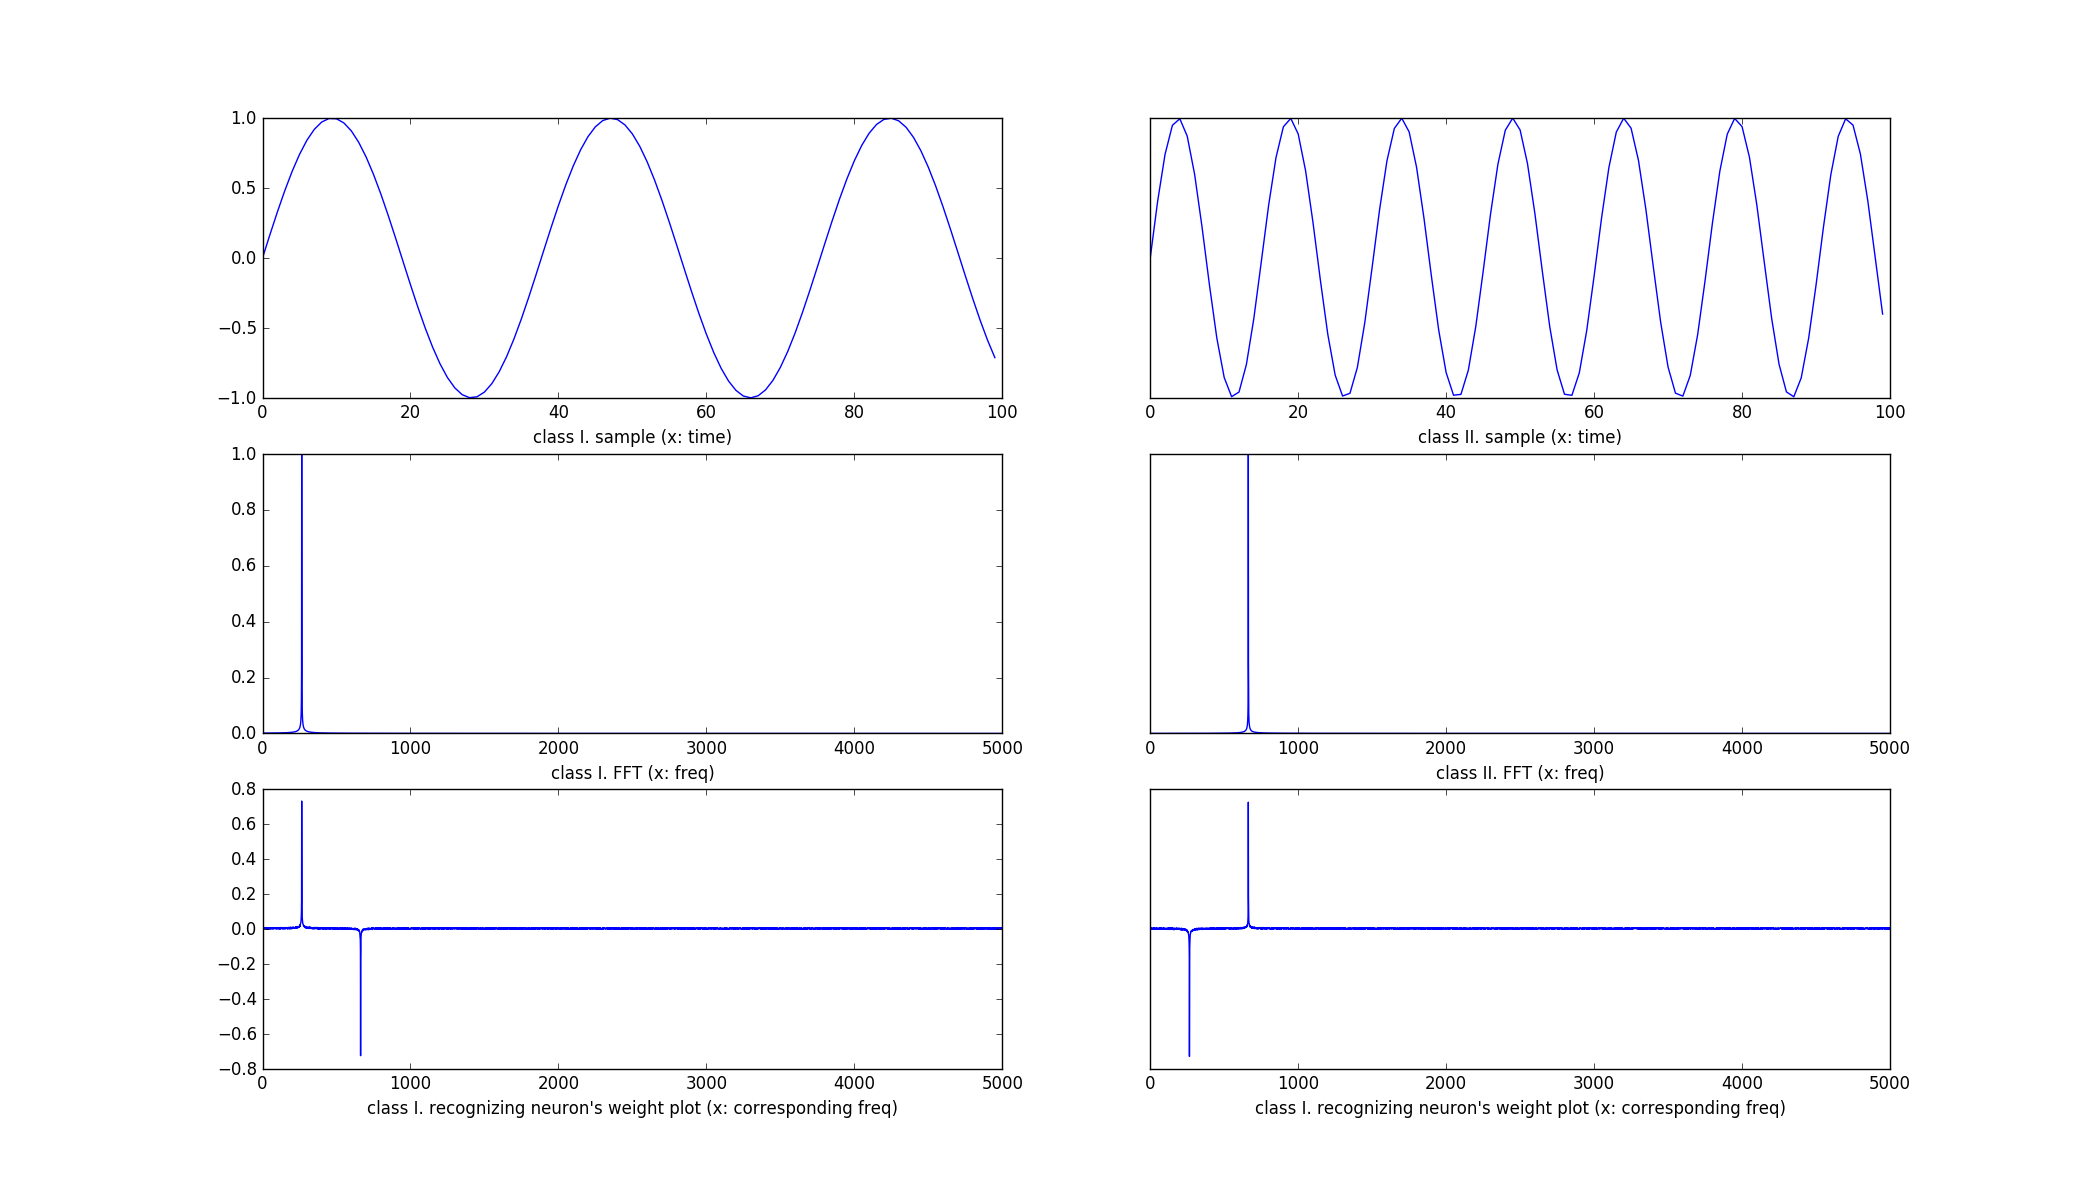
\includegraphics[width=0.8\textwidth]{N5000-L2e-1.png}
	\caption{The network's initialization and training parameters are identical to the network depicted on Figure \ref{fig:N5000}, only the transform precision is increased from $N=500$ to $N=5000$ resulting in more narrow spikes corresponding to the recognized frequency}
	
	\label{fig:N5000}
\end{figure}


\begin{figure}
	\centering
	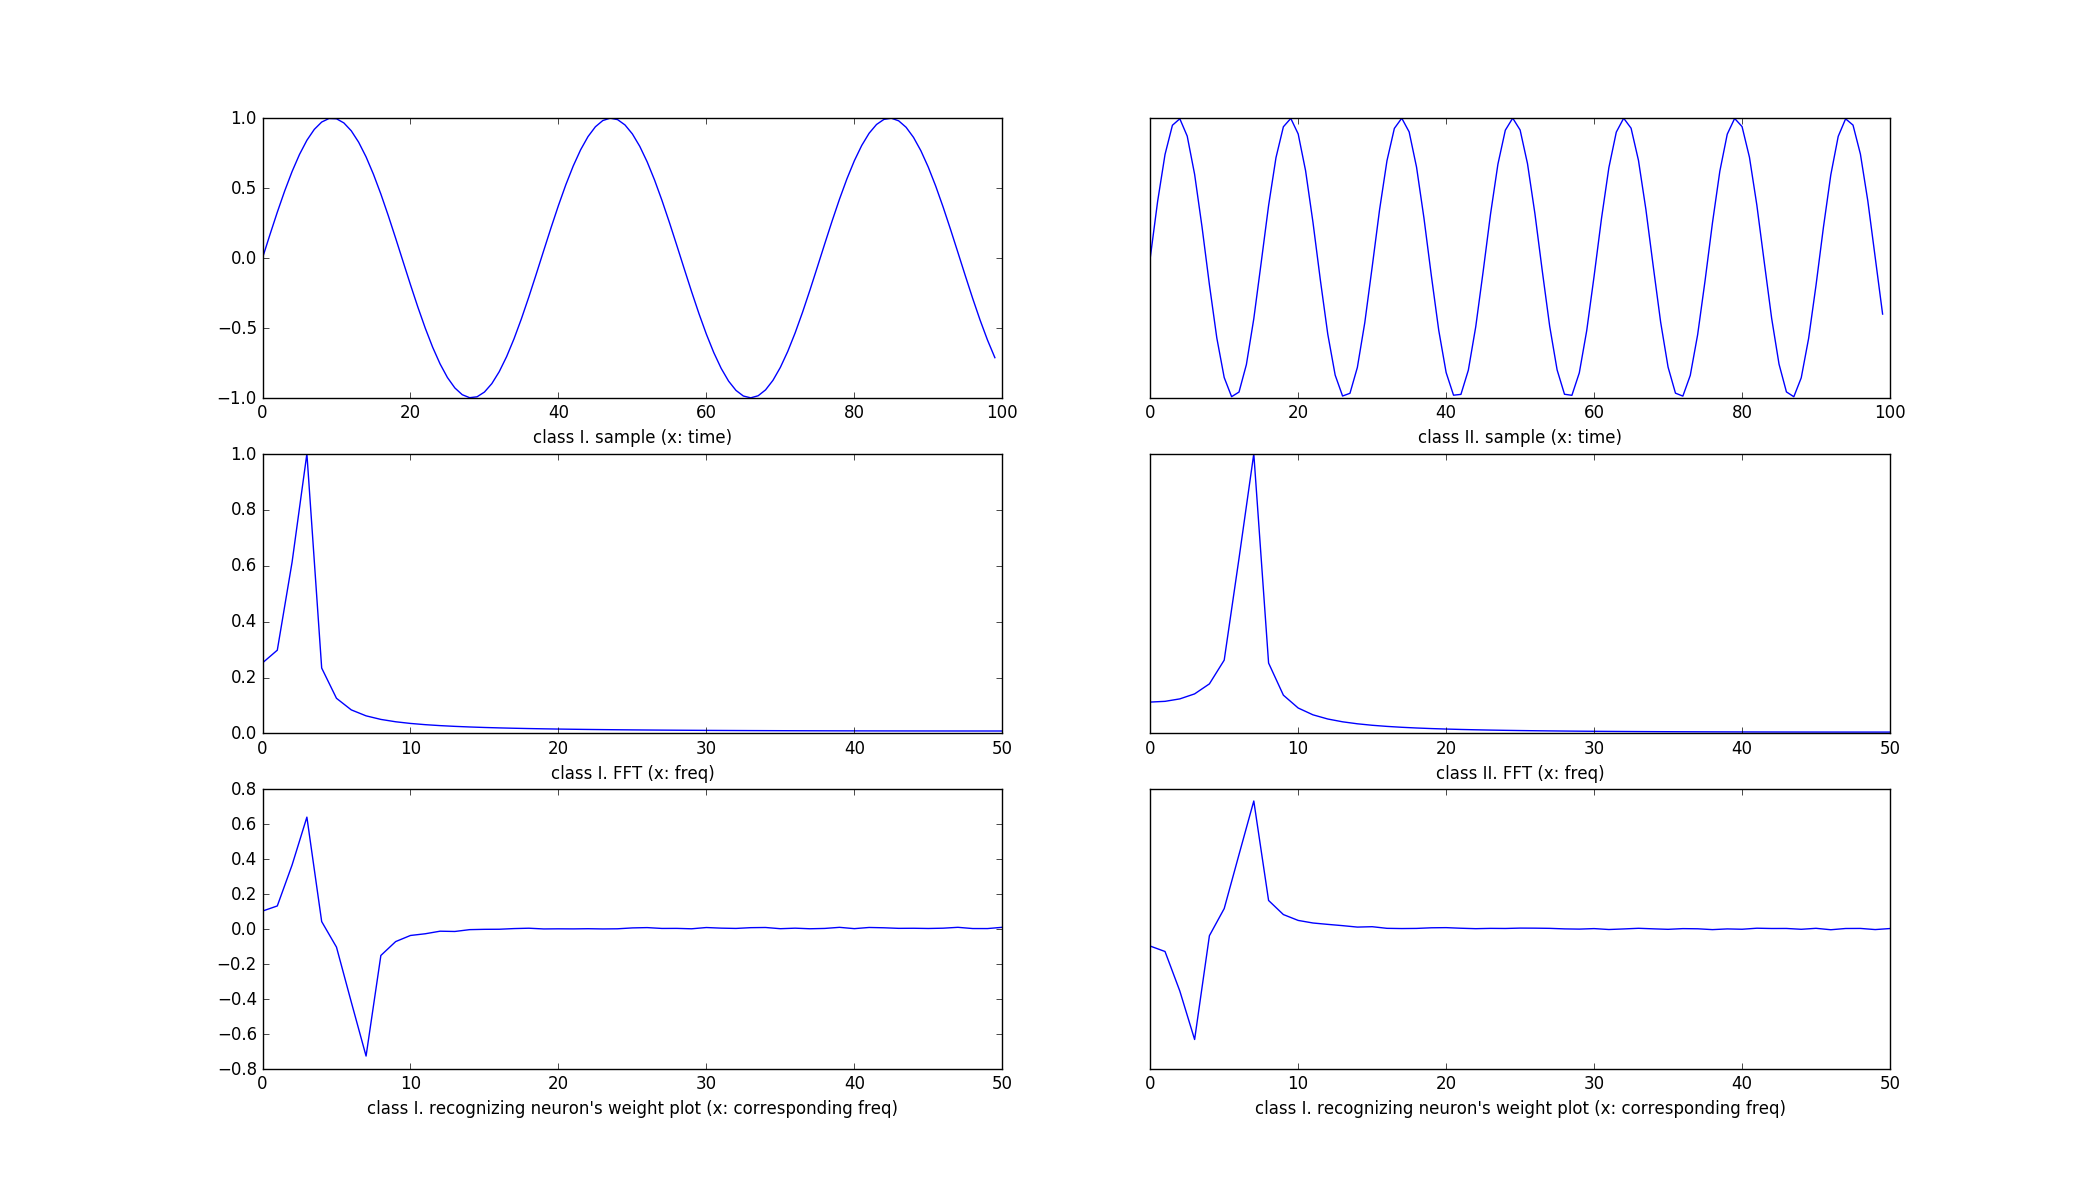
\includegraphics[width=0.8\textwidth]{N50-L2e-1.png}
	\caption{The network's initialization and training parameters are identical to the network depicted on Figure \ref{fig:N500}, only the transform precision is decreased from $N=500$ to $N=50$ resulting in more shallow spikes corresponding to the recognized frequency}
	
	\label{fig:N50}
\end{figure}

\begin{figure}
	\centering
	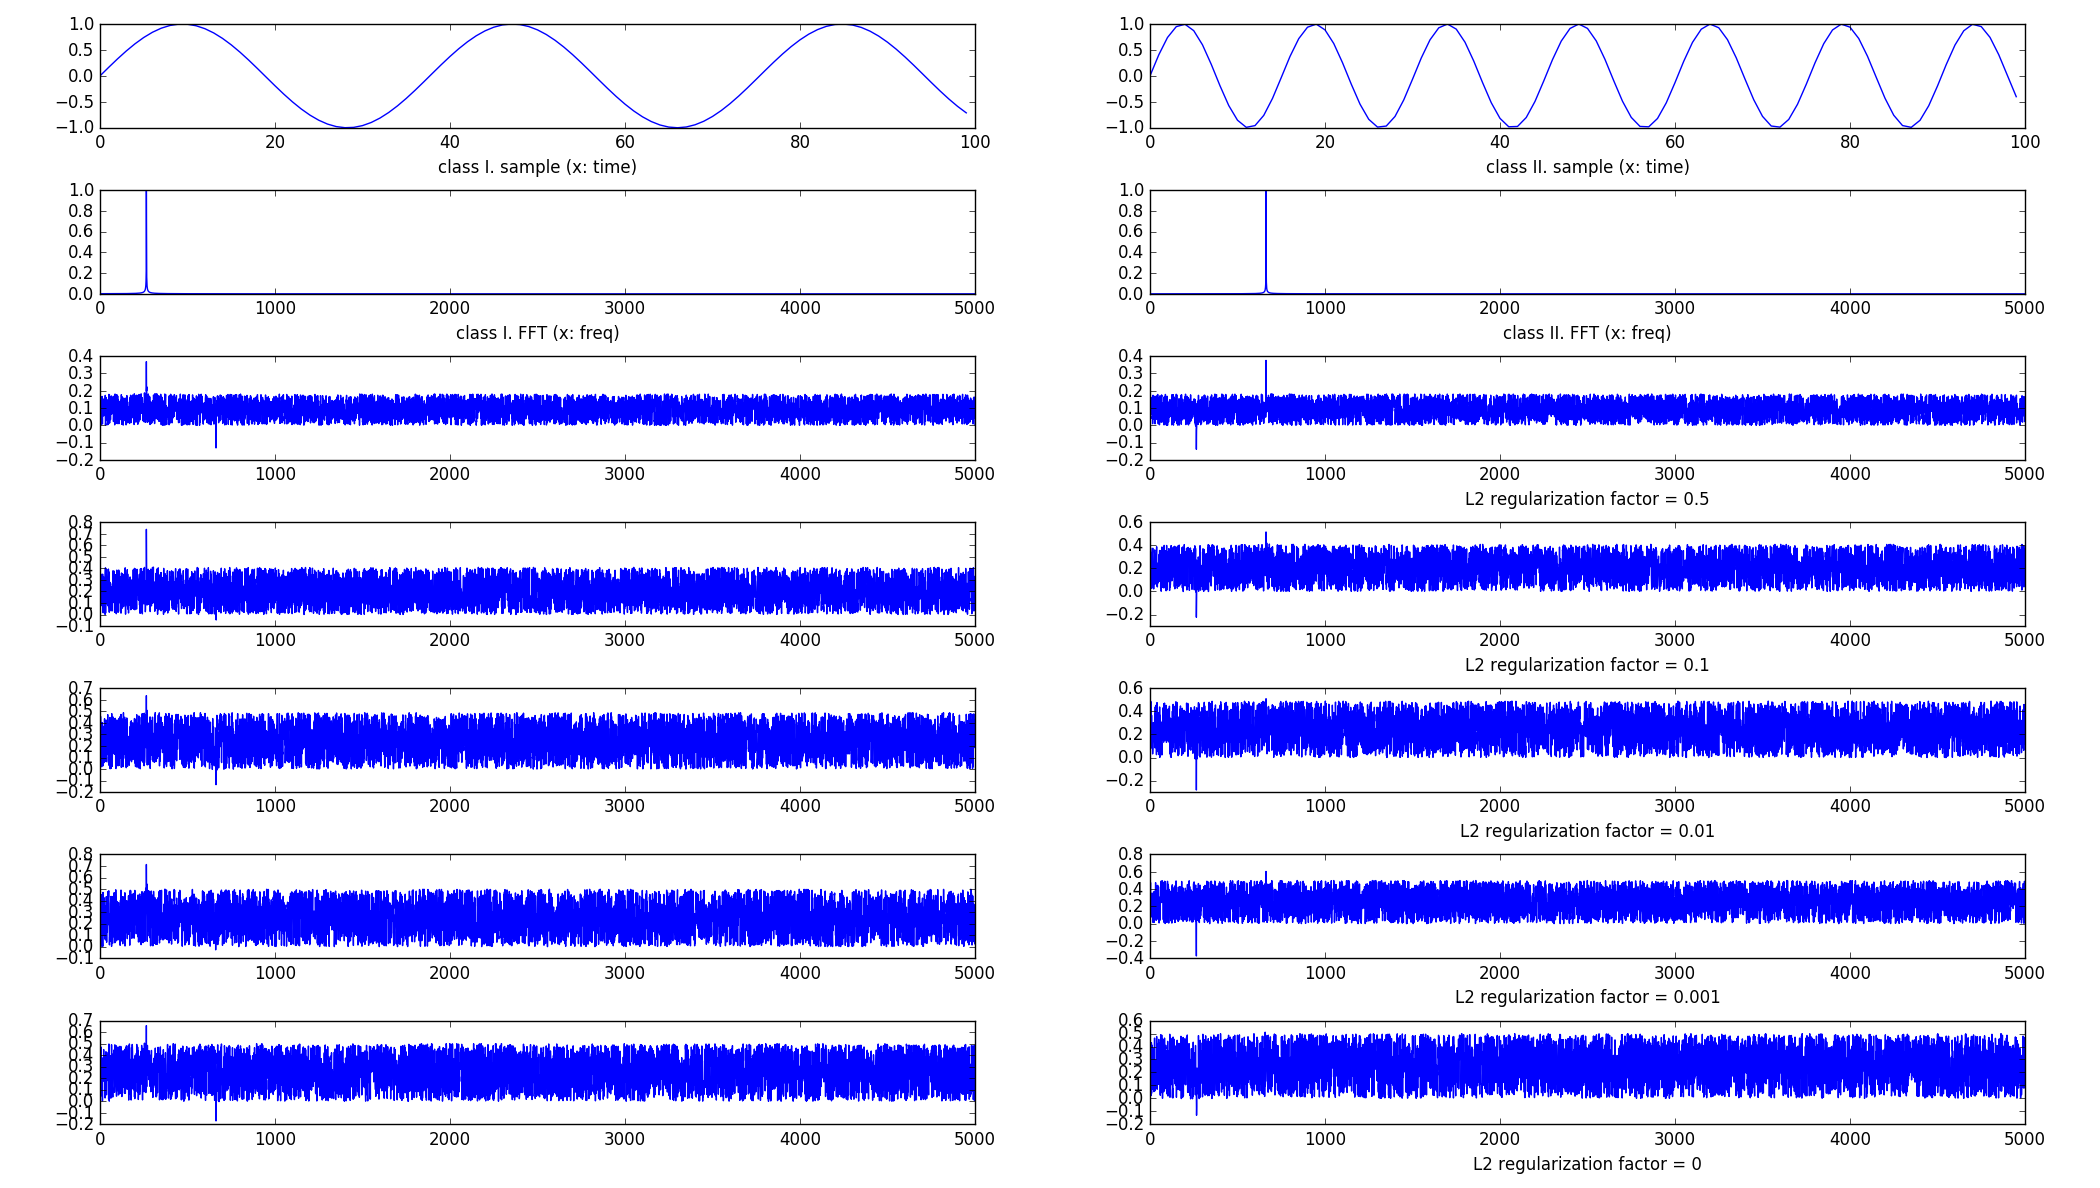
\includegraphics[width=0.9\textwidth]{L2_factor_plot--5epoch.png}
	\caption{After the third row the figure depicts independently, identically initialized and trained networks detailed in Figure \ref{fig:N500}, only the regularization factor $\lambda$ is decreased from $0.5$ to $0.0001$ resulting in more noisy weight plot. Still the  corresponding weights' magnitude are outstanding}
	
	\label{fig:reg}
\end{figure}

\begin{figure}
	\centering
	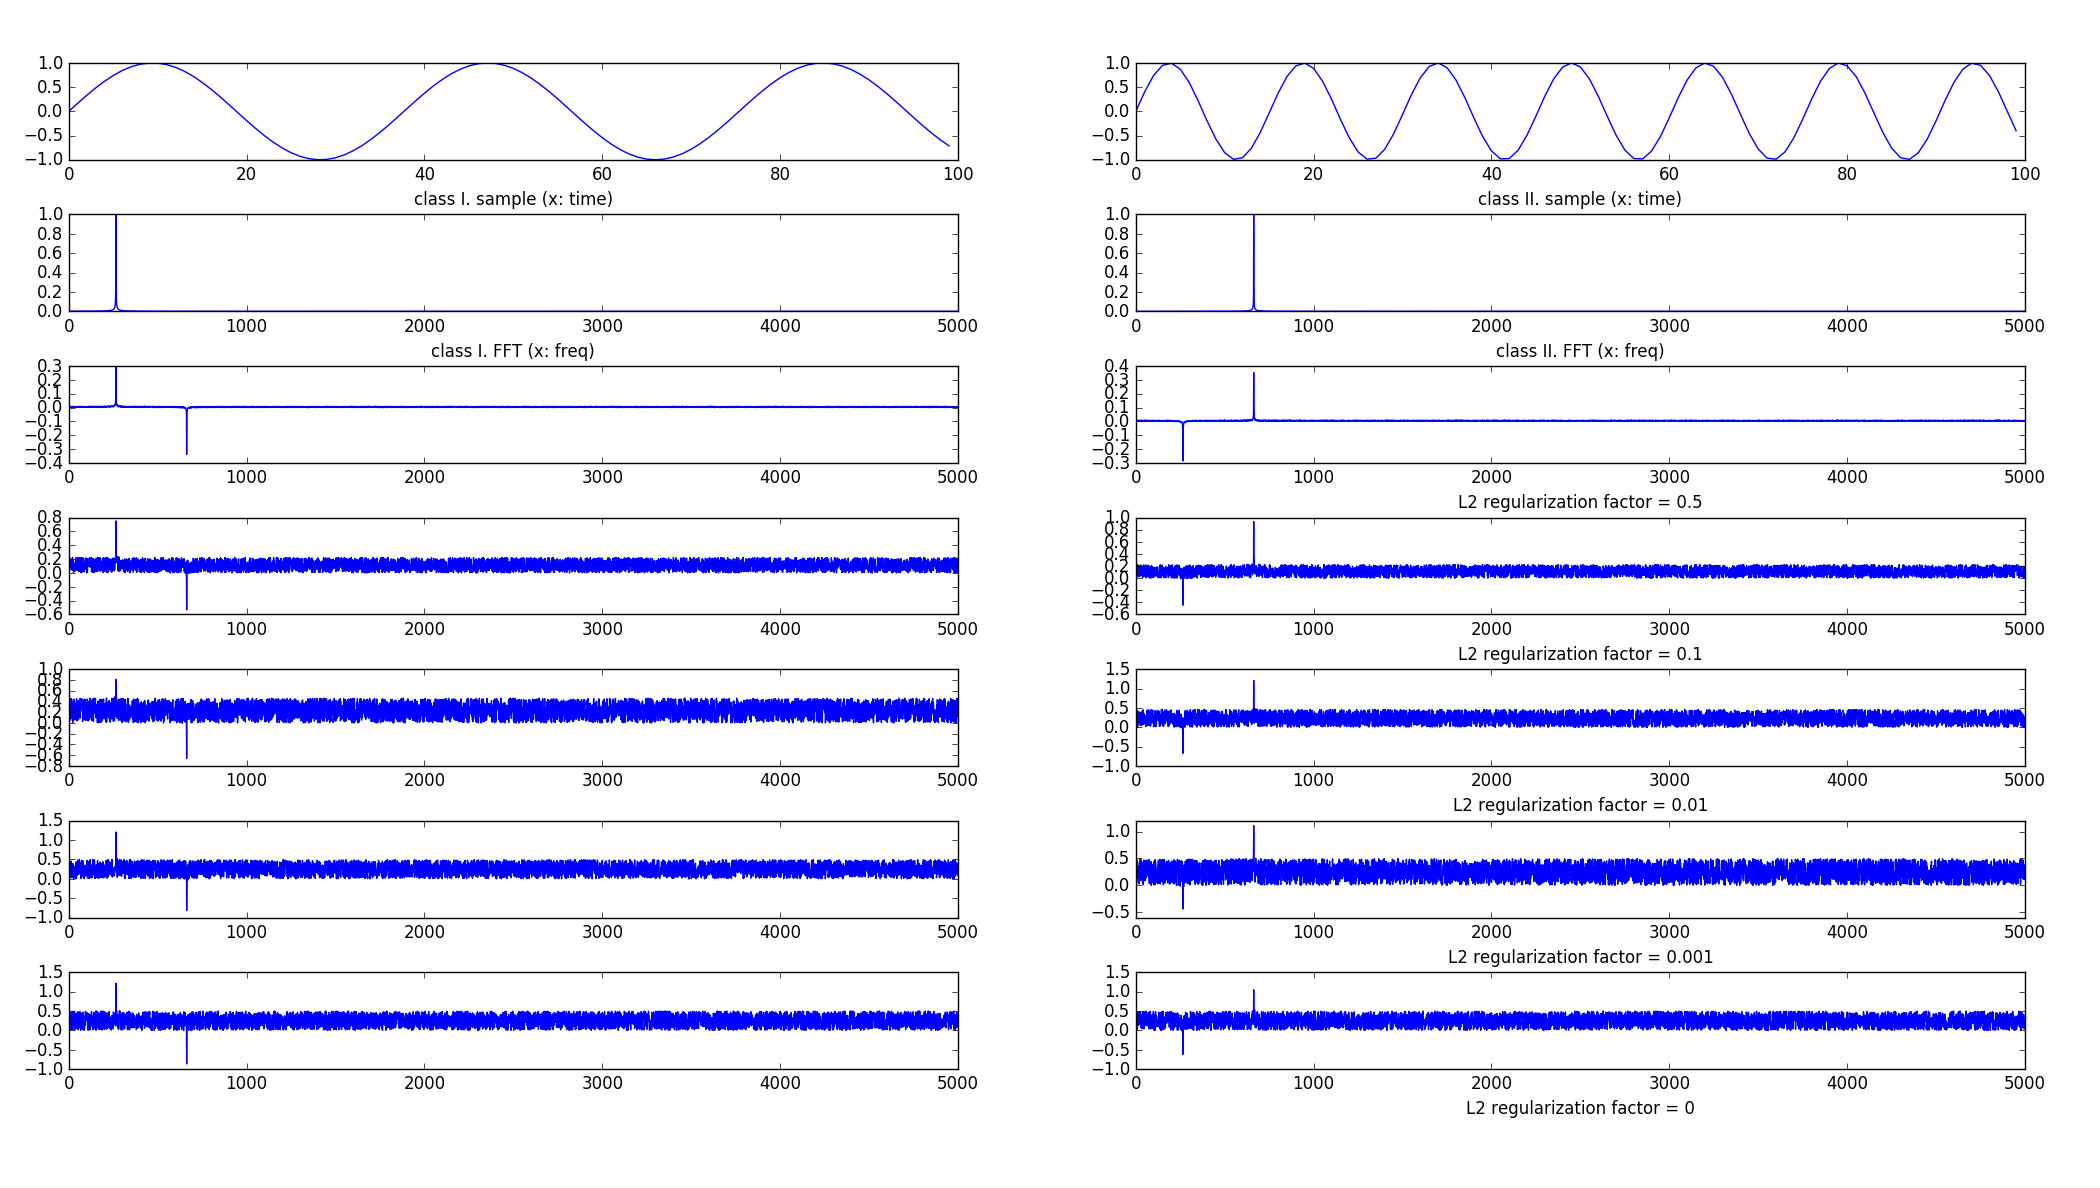
\includegraphics[width=0.9\textwidth]{L2_factor_plot.png}
	\caption{The network was trained with the same parameters as the one depicted on \ref{fig:reg}, except that it was trained for five times longer. Despite the result is quite the same as the result achieved with greater regularization factor, overfitting should be avoided. Overfitting occurs when the network $N$ tends to perform well on the training set, but fails to recognize unmet samples, because either the training samples were not general enough, either the network was just large enough to memorize each one of the samples, or both. }
	
	\label{fig:overtrain}
\end{figure}


\paragraph{Dealing with multiple waves}
Approaching real life problems, more parallel signals should be introduced to the network. In this subsection the case of recognizing overlapping frequencies and common frequencies are examined. The networks were initialized and trained identically to the network in previous experiment with $\lambda=0.5$. In the first case six different base functions were used to compose the samples. On Figure \ref{fig:multi} it is really trivial that the network is not just capable of separating low-pitch samples from high-pitch samples, but can recognize different patterns, even if they are scattered throughout the state space of the input. In the second case the conclusion is that the perceptrons (if well trained) will look only for relevant signals and patterns in the input.  See Figure \ref{fig:multi-common}

\begin{figure}
	\centering
	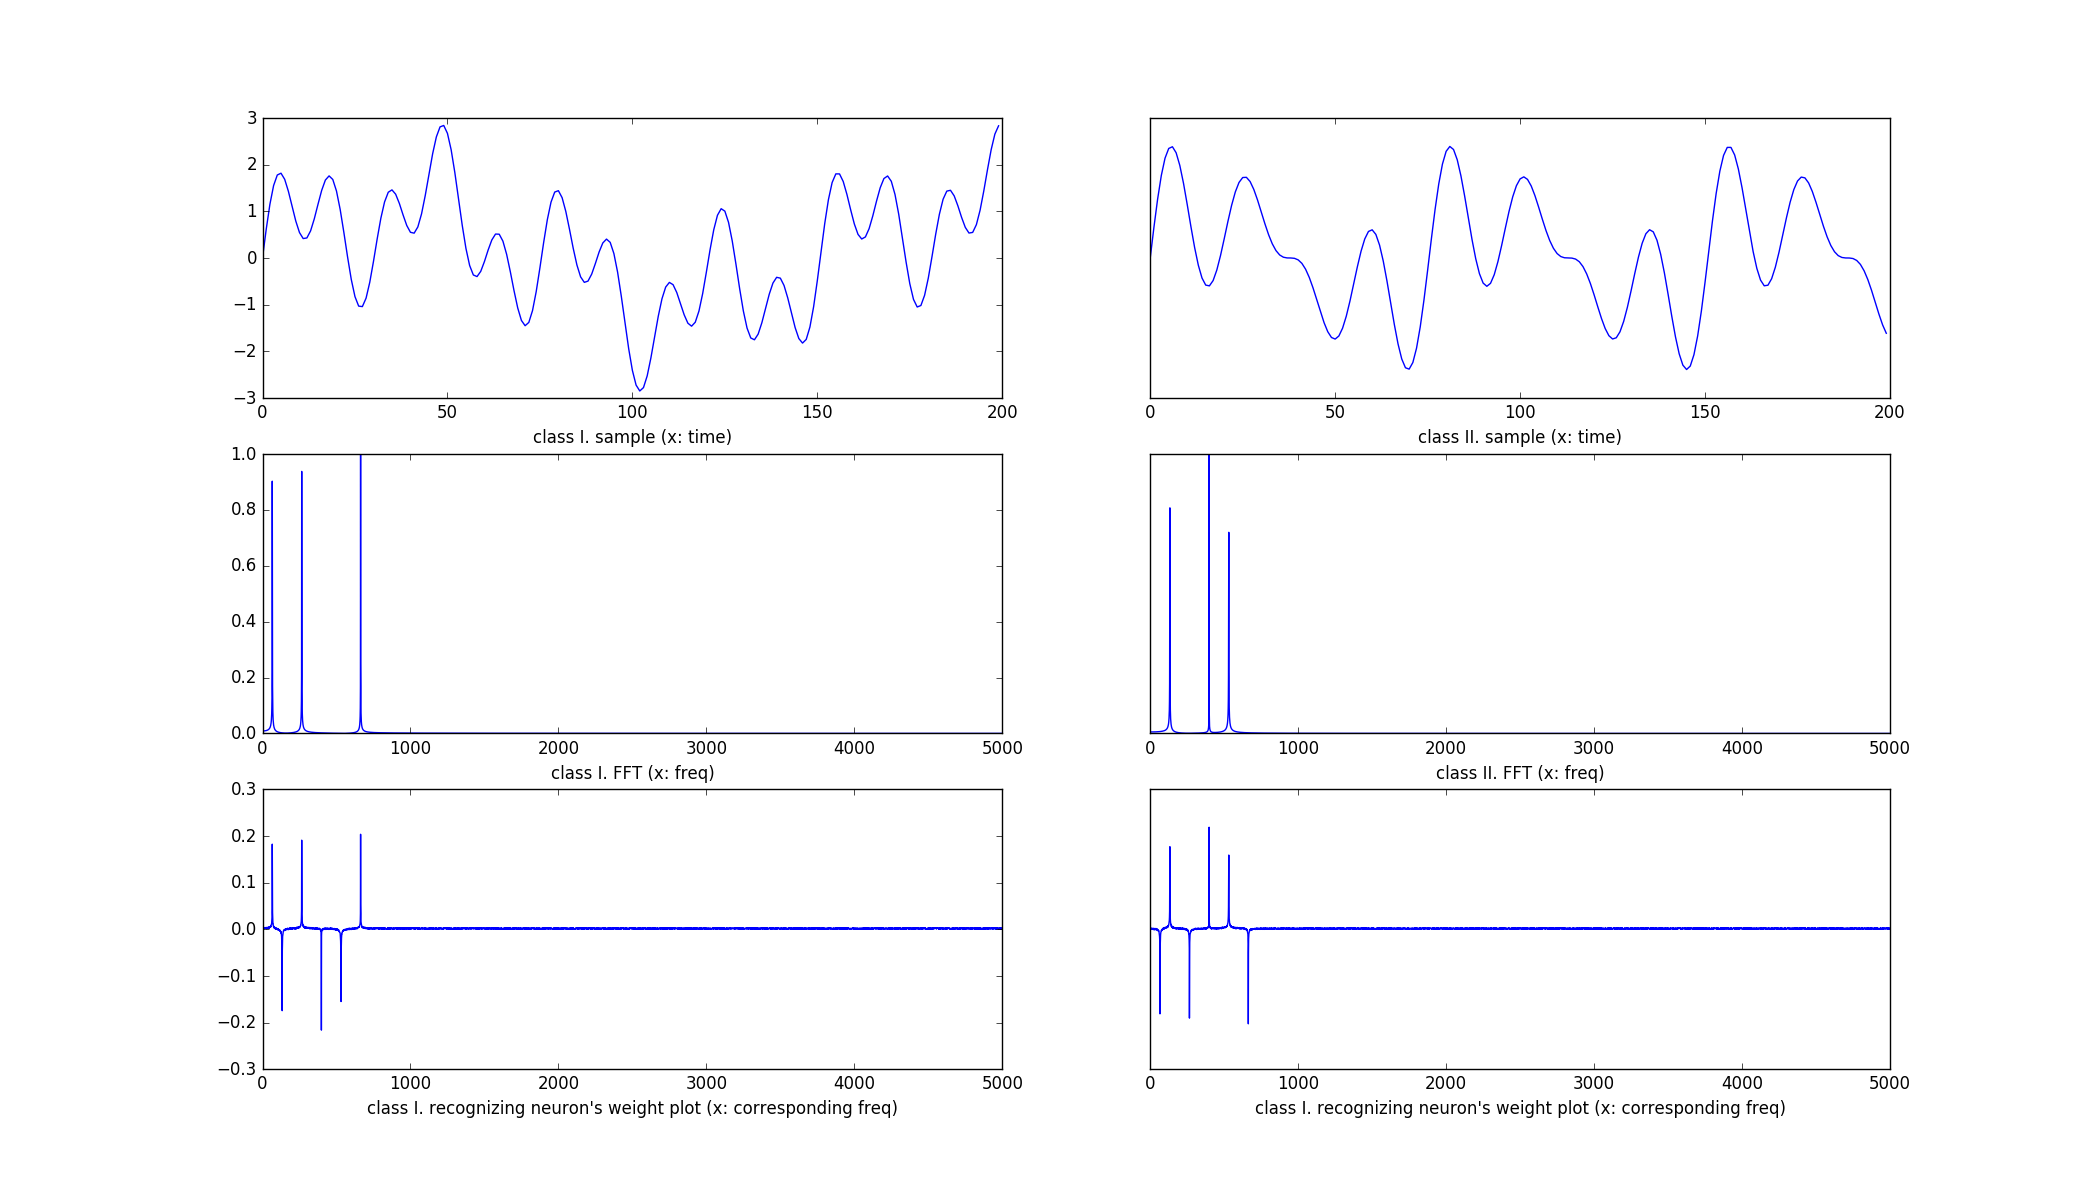
\includegraphics[width=0.9\textwidth]{multiple---N5000---L2-5e-1.png}
	\caption{Each sample is an equal combination of 3 independent sine function. The frequency of the waves are not separated to low and high frequencies, both can be found in each sample, but it is important to notice, that the two samples do not have any common component.}
	
	\label{fig:multi}
\end{figure}


\begin{figure}
	\centering
	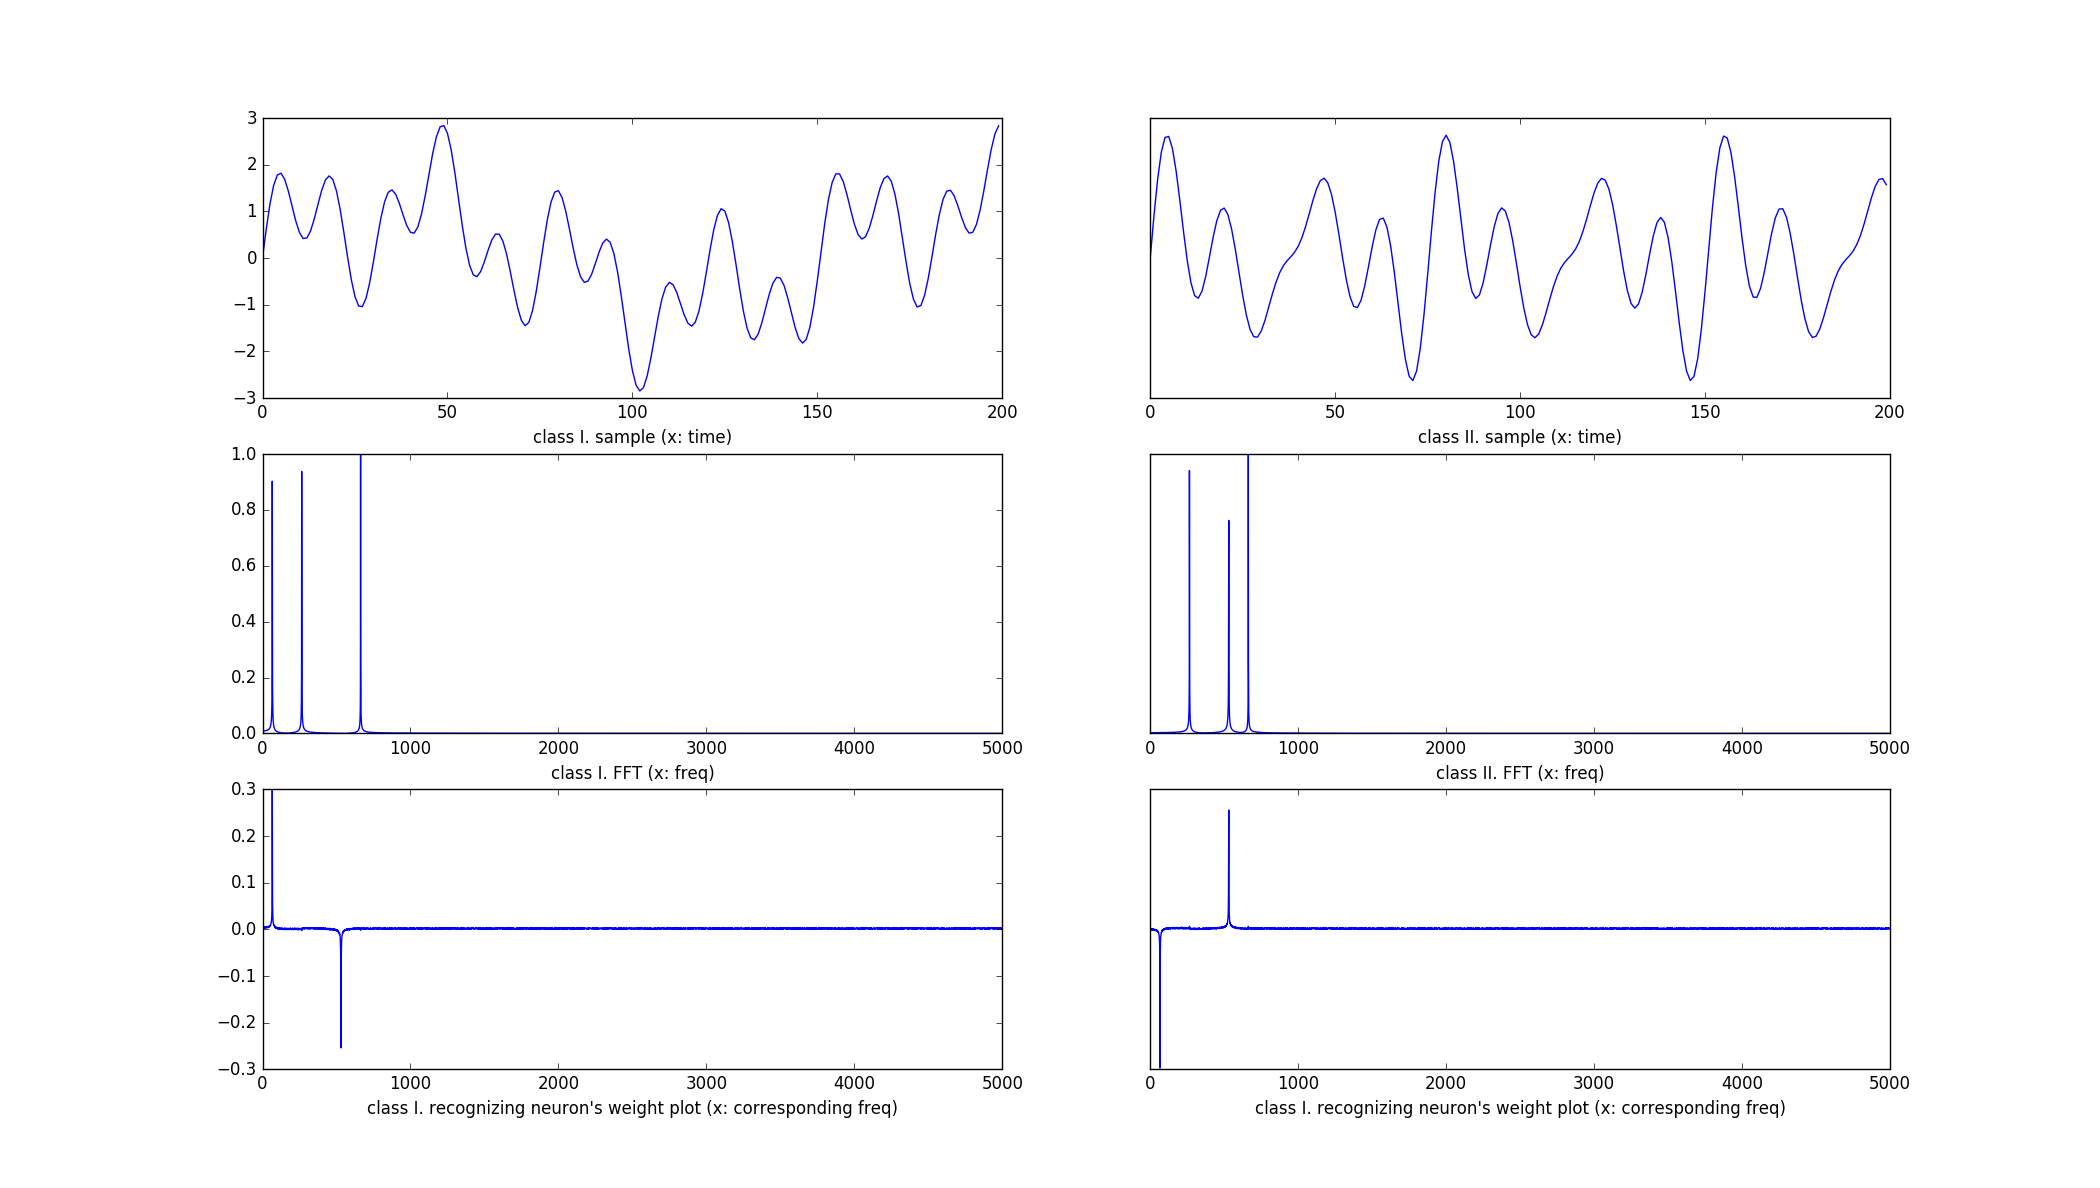
\includegraphics[width=0.9\textwidth]{multiple--common-20-50Hz--N5000---L2-5e-1.png}
	\caption{In opposite to the case depicted on Figure \ref{fig:multi} here the samples have two common component, meaning that in the base functions there are two common frequency and only differs in one harmonics. The result is that the common features extracted by the FFT are discarded, and the perceptrons only learn the difference.}
	
	\label{fig:multi-common}
\end{figure}

\paragraph{Introducing Regularization.}
Regularization is simply a practical implementation of Occam's razor, meaning that the unimportant features of $\mathbf{x}$ will not be taken into account by the perceptron. 

On Figures \ref{fig:N500}, \ref{fig:N5000}, \ref{fig:N50} the weights were originally initialized with random Gaussian noise, but after training only the important frequencies' weights stayed significant. 
If the regularization factor is reduced the noise wouldn't disappear and the perceptron would still take irrelevant information into account. 
This phenomena is shown on Figure \ref{fig:reg}. 
However, instead of regularizing, we can \emph{over train} our networks, increasing the number of epochs, the number of times we show the same samples in the training set. 
Noise reduction via \textbf{overfit} can be seen on Figure \ref{fig:overtrain}. 

\subsection{Real Samples}
For acquiring samples from the environment the architecture should be wired to a physical sensor which will transfer signals from analog to digital. 
Practically external libraries are applied to perform the capturing. I used PyAudio. PyAudio provides Python bindings for PortAudio \cite{pham2006pyaudio}. 
The only thing remaining is to write an adapter to make the information format compatible with the network's architecture.

\paragraph{Capturing sound}
For the following experiments an algorithmic smart capturing is used, which enables us to record multiple sound waves with different length, without pressing a single key. The main idea is that the noise of the environment can be monitored, and in the background mean averaged. A practical threshold is set for recognizing significant audio inputs, where the magnitudes of the sampled waves reach the critical. After the recording starts, a fixed size time-frame will cancel out further activities of the capturing system. Another option is to end the capturing process when the magnitude of the input falls below a threshold. Either way, the samples are gathered in a list, and each of them are transformed to frequency domain with \emph{N-FFT}, producing equal length inputs  $\mathbf{x^i}$ for the network.

\paragraph{Defining the classes}
For human interpretation it is useful, that the separated classes are labeled, while from the aspect of the network it is totally irrelevant what the classes represent. That is an important thing to understand, both in supervised and in unsupervised learning. In the next cases separation sound waves of \emph{Hello} will be separated from samples of \emph{Goodbye}.

\subsection{Binary classifiers}
\paragraph{First greeting recognizer}
The first model trained on greetings and farewells is working as expected. In the demo found at \cite{DV} \url{~/demo/audio/so.py} the user is asked to input number of $N$ samples representing class I, and the same number from class II which will be labeled with the assumption that the samples do not overlap. The length of the samples can vary in time, because the smart capturing takes care of the preprocessing. 
For ending the recording session produce some loud noise, a clap should do. 
The labeled samples are then taken into account as the training set for the network, and the process adjusting the parameters begins. 
After 30 epochs of training the network waits for new $\mathbf{x}$ to classify. 
A few tests can be made to ensure the network is working well. 
My results with N=1000, on 3-3 input sample is performing around 91\% (100 tests were performed in total). 
Sending a \textbf{\textsc{sig-term}} will end the testing session and a summary window will pop up, probably something like on Figure \ref{fig:hello}.

\subsection{Multiclass classification}
\paragraph{Recognizing greetings in multiple languages}
Currently the model works like the one depicted on Figure \ref{fig:dumb}. 
A real task can be defined, where the network $\mathbf{N}$ has to classify in which language the user said hello. Unfortunately there are more languages than two, but neural networks are flexible enough to be able to recognize and separate the inputs into  $N$ number of classes. For the improved model see Figure \ref{fig:improved} 

The experiments were done with 5 different languages: \emph{French, Arabic, Spanish, German, Hungarian}. The training scene is the same as in the previous cases: input sequentially $N$ number of samples for each language, end the recording with a clap.
For a demonstration script check out \cite{DV} \url{~/demo/audio/nclass.py}.
The network trains on the given set, and the system is ready for testing.

With the following hyperparameters: 1-1 number of samples in each language, \emph{mini-batch}$=1$, \emph{number of epochs}$=15$, $\lambda=0.005$, from random Gaussian initialization a network with 60\% performance can be obtained.
\emph{Note}: at first 60\% may sound only slightly better then the 50-50 guessing, but considering the fact that the random guess would be distributed now between 5 classes, resulting in 20\% hit-rate, meaning that only every fifth greeting would be classified correctly. 
Compared to that, 60\% is much better -- the network is tells the good answer in more than half of the cases.

With larger training set, 3 samples for each language the result raised over 85\%. Comparing to industrial networks the training set used to adjust the parameters is very small in size. 
For larger projects usually the training set contains thousands and millions of samples, and overfitting is less likely to occur. 
For such a narrow network trained with a poor training set it can be said that 85\% is not that bad at all. Although the result still depends on who tests the configured network.

\begin{figure}
	\centering
	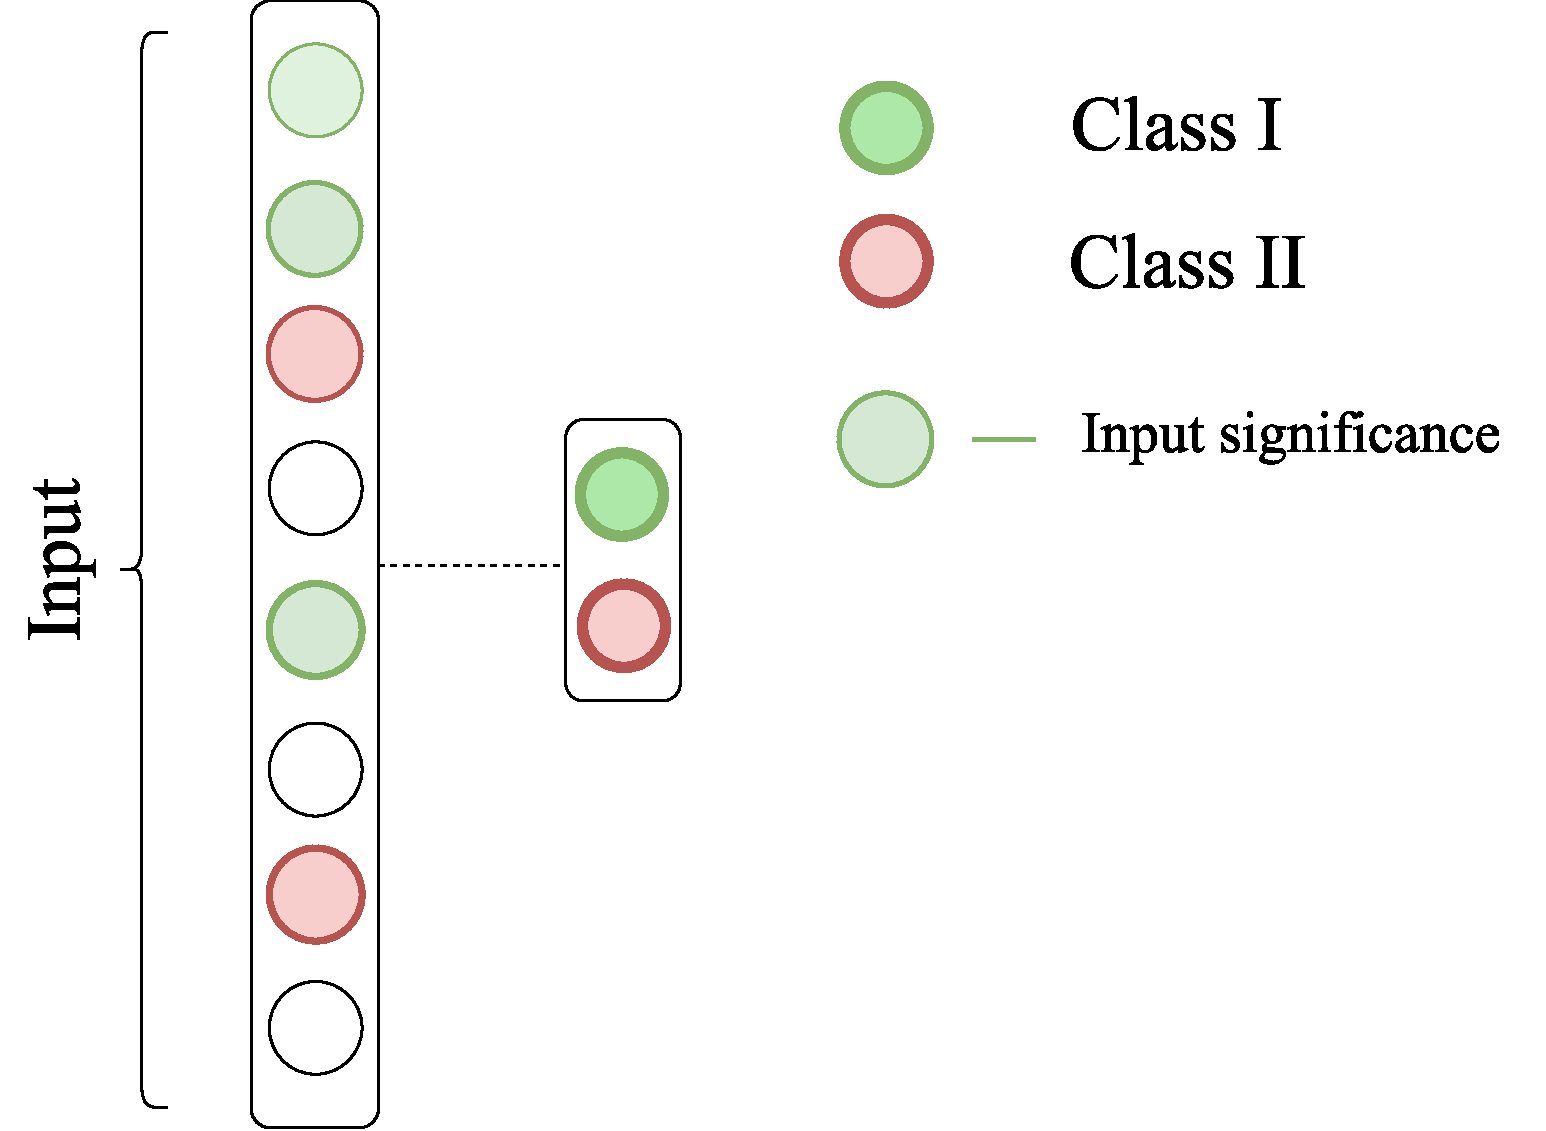
\includegraphics[width=0.5\textwidth]{current-model.pdf}
	\caption{A basic perceptron model, operating on 8 clues of the input. The perimeter of each input node describes how much it increases the output of the perceptron with the same color and decreases the neuron with opposite color. Input nodes which are not colored holds irrelevant informations for both perceptrons, therefore discarded.}
	
	\label{fig:dumb}
\end{figure}

\begin{figure}
	\centering
	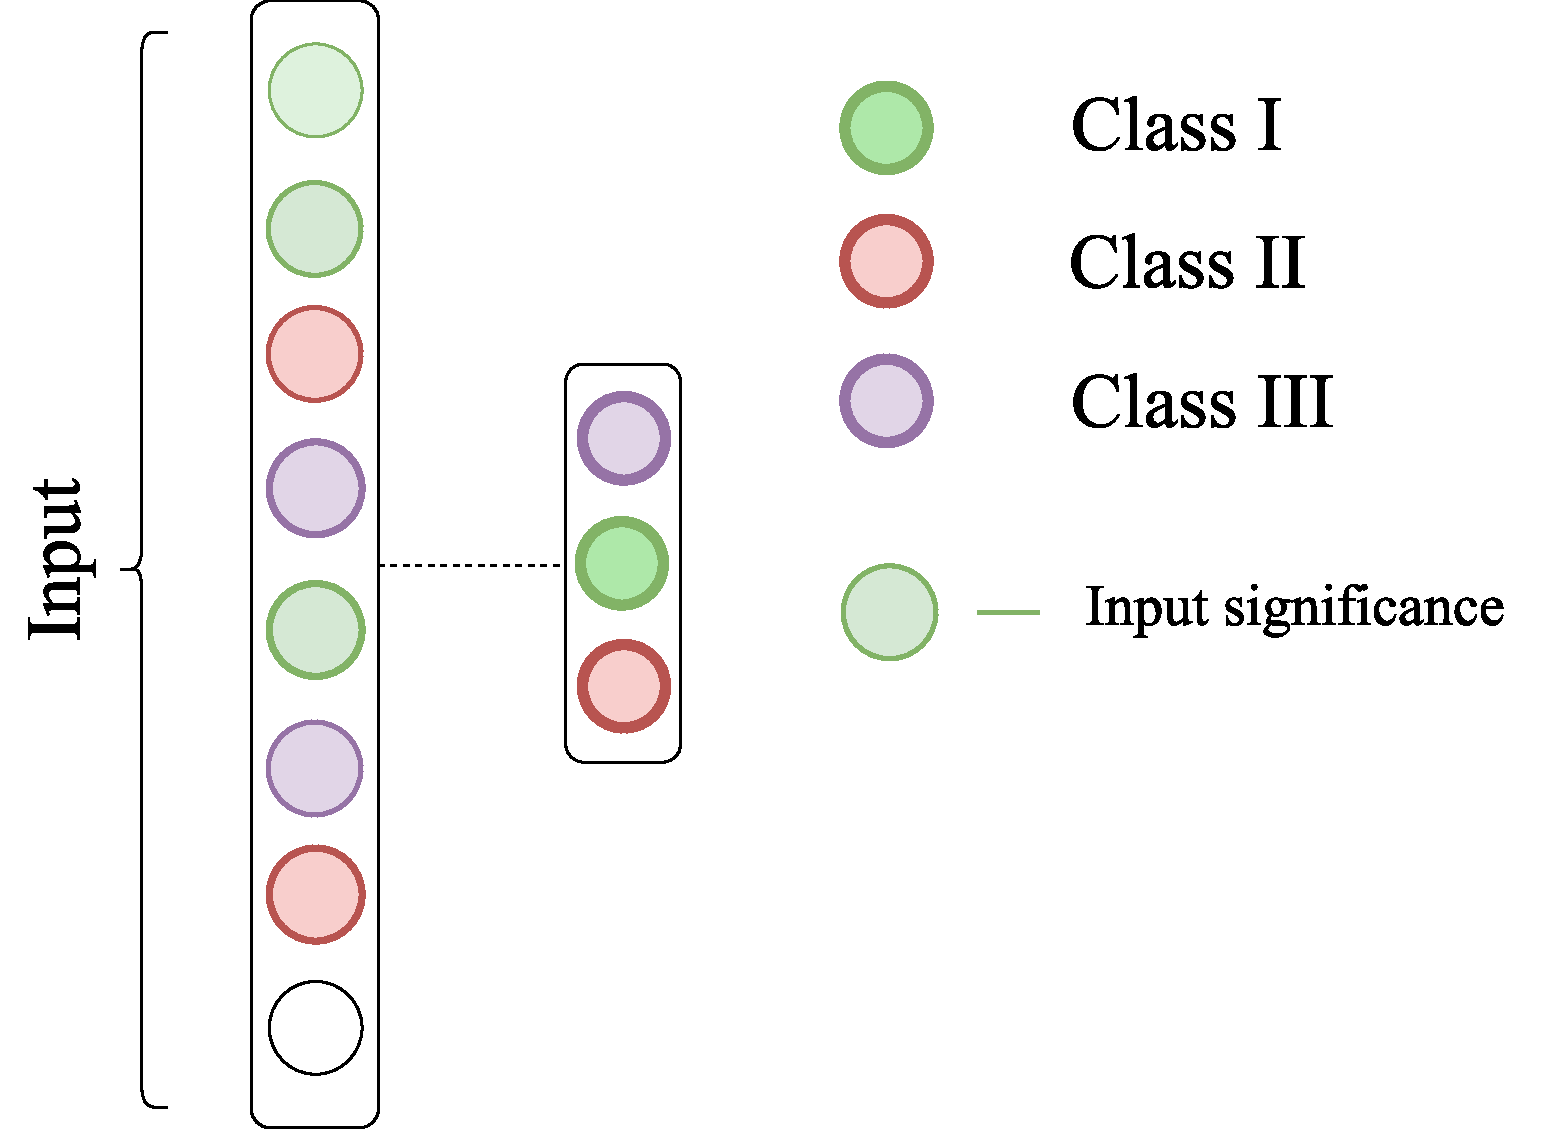
\includegraphics[width=0.5\textwidth]{improved.pdf}
	\caption{An improved perceptron model, operating on 8 clues of the input $\mathbf{x}$ , deciding which class it belongs to. The weight anti-symmetry is not so trivial in this case because perceptrons of multiple classes can be turned on by one single feature while other perceptrons are inhibited by the same feature or may even discard it. Meaning that the colors on this figure are a bit tricky, because each input node can be shared between the classes.}
	
	\label{fig:improved}
\end{figure}

\subsection{Conclusion}
So far it was shown how single layer neural networks work. 
How they should be thought of, what difficulties arises during their training. 
The capabilities of shallow networks were met during tests with the N-multiclass classifier. 
The next topic of the investigation is that how can these perceptron layers be combined to each other, 
for example to recognize whether a user said yes or no, without explicitly telling  which language he or she was speaking.

\begin{figure}
	\centering
	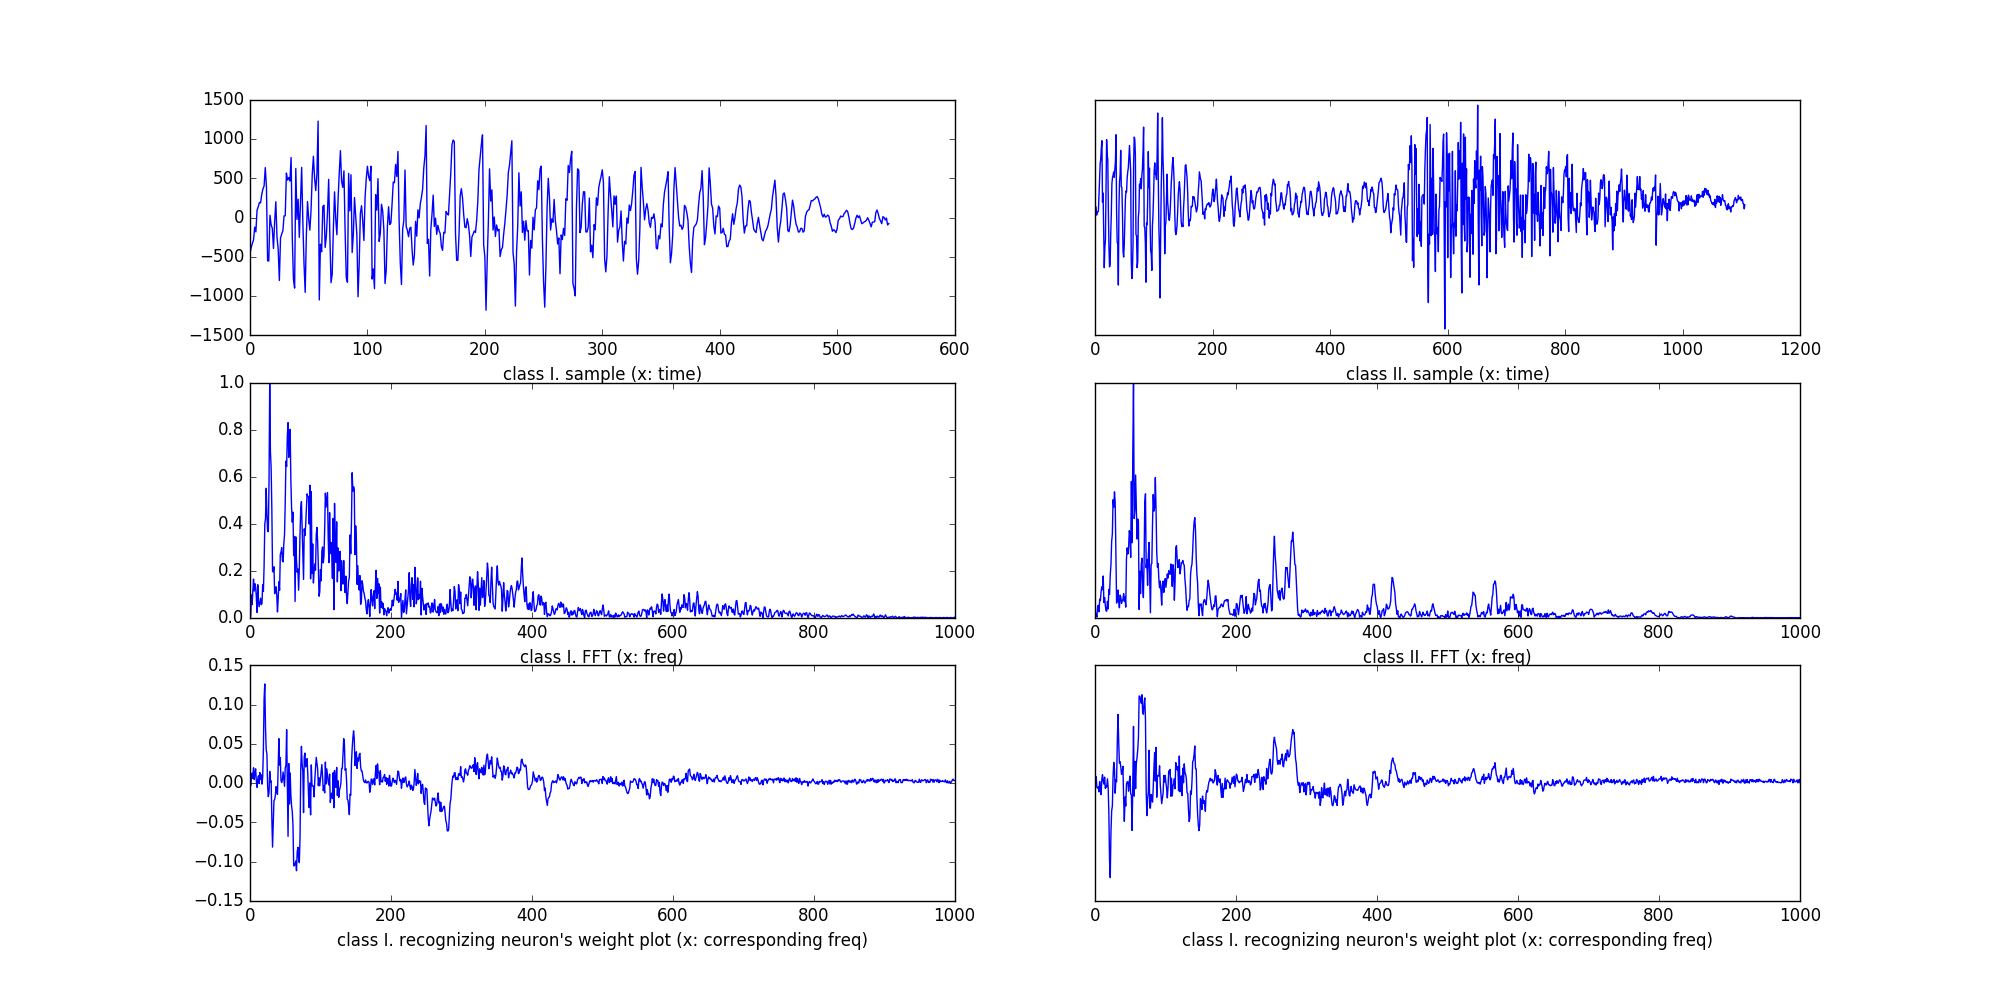
\includegraphics[width=\textwidth]{hello-goodbye-N1000-L205}
	\caption{On the left: the first example of the whole training set, showing the wave and frequency plot of a \emph{Hello}. On the right: the same for the word \emph{Goodbye}. guesses more than half 
	As experienced on Figure \ref{fig:N500}, an anti-symmetric pattern arises in the weight plot of the classifier perceptrons. 
	One pattern in the frequency domain of \emph{Goodbye} samples is very dominant and the weights of the \emph{Goodbye}-recognizing perceptron fits on it very well, while the same pattern can be found in the opposite perceptron's weight plot with negative sign.}
	
	\label{fig:hello}
\end{figure}

\begin{figure}
	\centering
	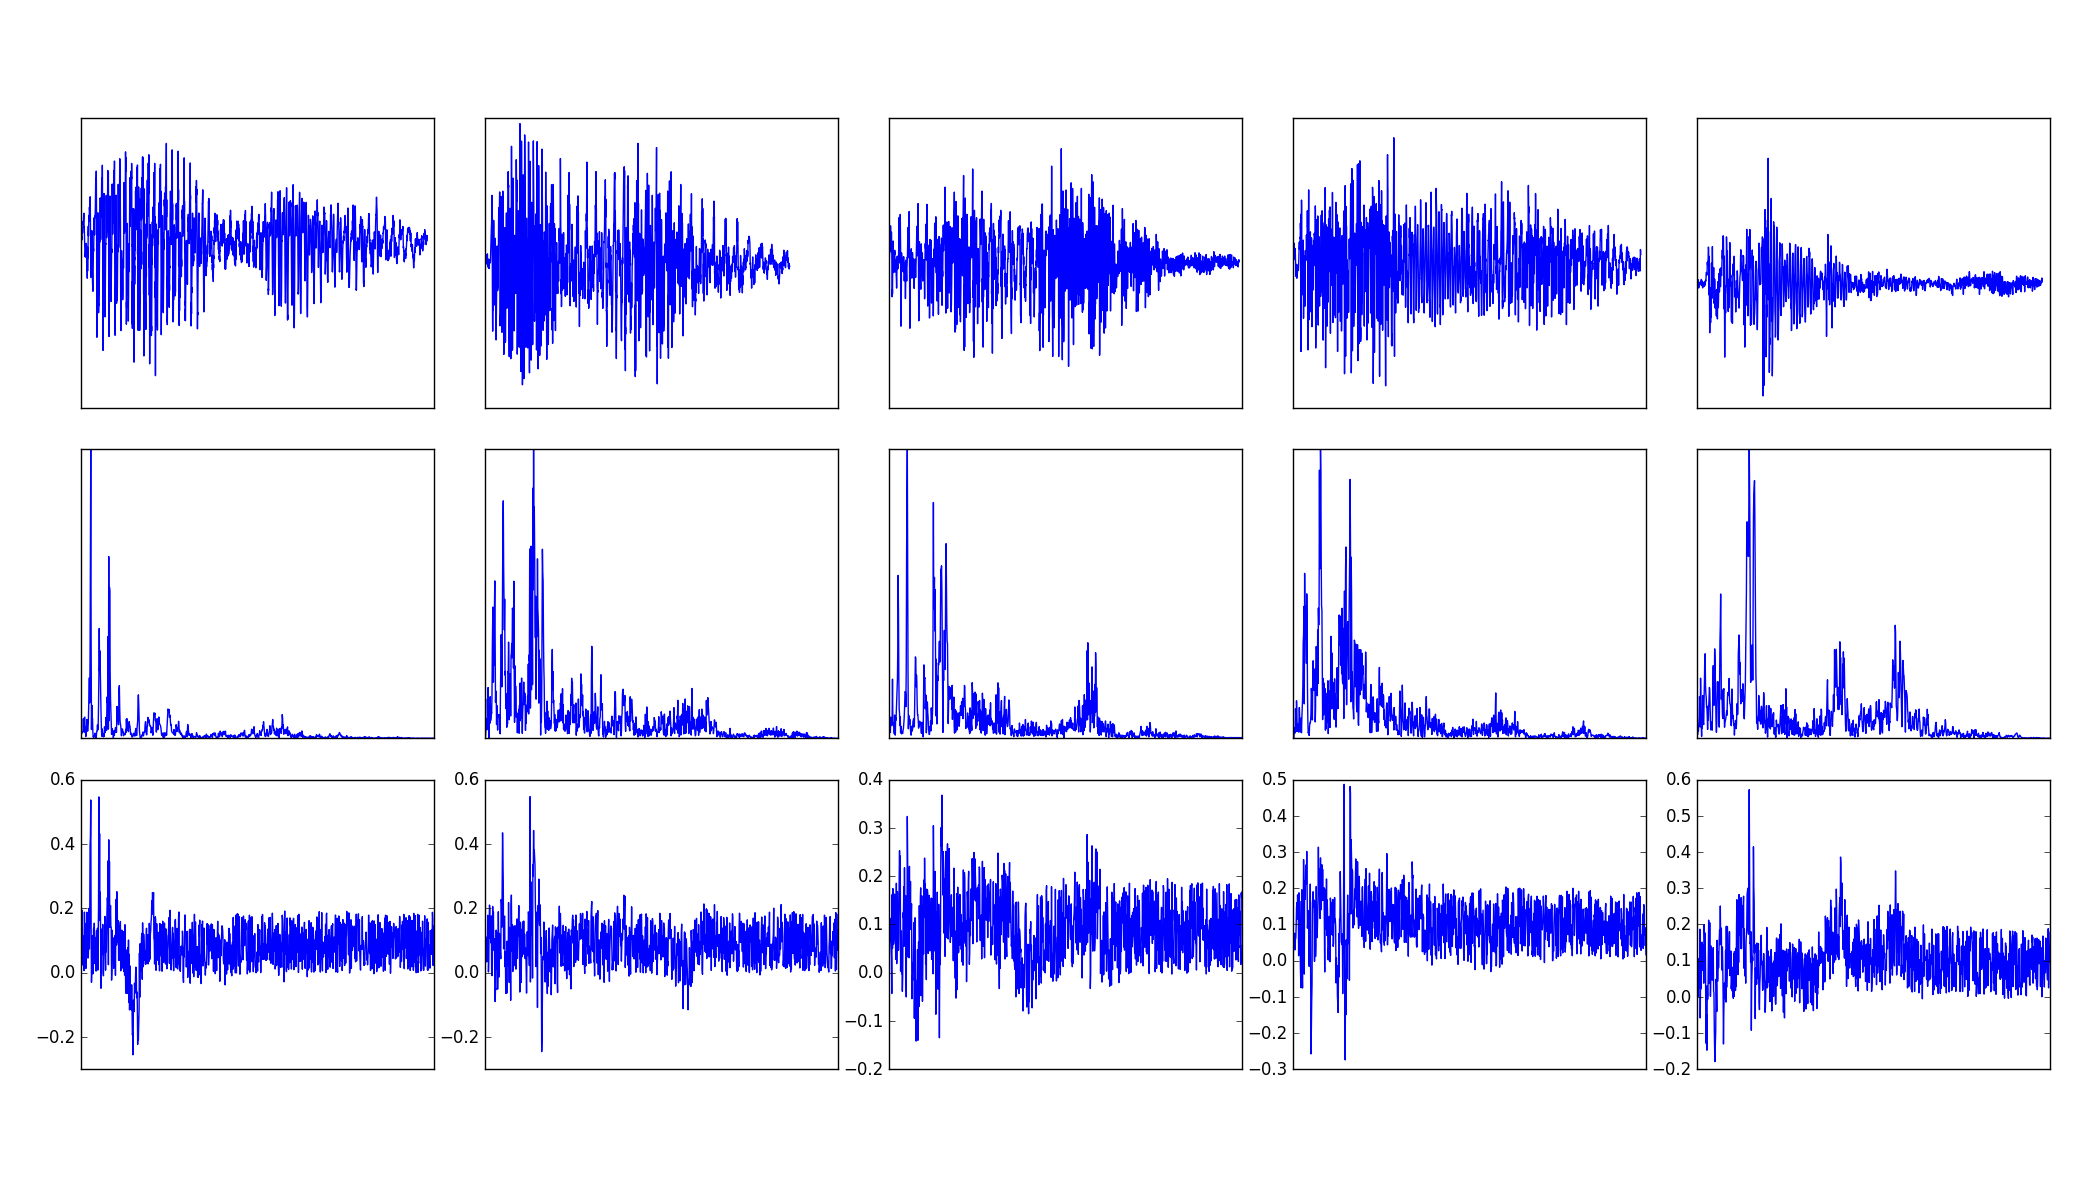
\includegraphics[width=\textwidth]{hello-5lang-3each}
	\caption{On this figure the sample time, frequency and the perceptrons' weight plots are depicted of the network that recognizes greetings in 5 languages. For human eyes it is hard to tell from either the time and frequency domain plot the corresponding language. The recorded greetings were sampled by me saying \emph{Bonjour, Salem, Hola, Halo} and \emph{Csá}}
	
	\label{fig:hello5}
\end{figure}

\clearpage

\clearpage
\section{Visualizing handwritten digit recognizer}
First layer can be easily visualized by just simply reshaping the weights (see Figure \ref{fig:regression}), but extracting patterns which are recognized by further layers are not trivial. The main goal is to find an algorithm which with the input images can be enhanced to highlight the patterns that causes strongest activation in each neuron.


\begin{figure}
    \centering
    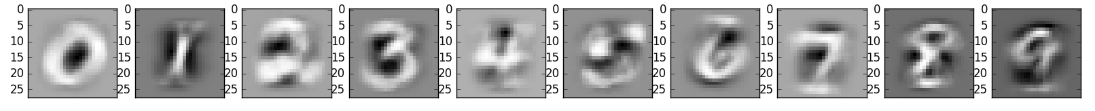
\includegraphics[width=\textwidth]{regression.png}
    \caption{Logistic regression: single layered network trained with $L_2$ regularization can be easily visualized, because the classifier neurons are strictly connected to the input pixels. Therefore by just simply reshaping their weights to make a $28 \times 28$ image will exactly show, what each neuron is looking for on the pictures.}
    \label{fig:regression}
\end{figure}

\subsection{Training}
\label{train}
The networks were trained on the MNIST dataset \cite{mnist}, with varying the following hyperparameters:
\begin{itemize}
    \item Number of total neurons, with different distribution between layers
    \item Number of hidden layers
    \item Learning rate - constant during epochs
    \item Regularization - $L_p$
\end{itemize}

The experiments width shapes and corresponding results are shown on \emph{Figure (\ref{fig:even}, \ref{fig:dec}, \ref{fig:inc})}.
In the very beginning it turned out that networks with 3 layer are the most stable for MNIST character recognition. 
Shallow networks, with fewer layers that had theoretically larger capacity than 3 layered ones, were unable to generalize the digits.
Deeper networks, with more layers either were numerically unstable, and exhibited vanishing gradient, or overfitting occurred early in the training process.
The 3 layered networks were trained with the following constraints: Stochastic gradient descent with $mini-batch=64$, learning rate $\epsilon = 0.05$ and total number of $epochs=25$.
Despite the varying capacity, the results rather depend on the shape of the network. The best of the three networks are compared in \emph{Figure \ref{fig:comp}} 


\begin{figure}
    \centering
    \includegraphics[width=0.9\textwidth]{shapeNN-even.png}
    \caption{Evenly distributed networks don't the input, even the last layers tend to activate on various input patterns. During backpropagation the gradient is also more likely to disappear.}
    \label{fig:even}
\end{figure}
\begin{figure}
    \centering
    \includegraphics[width=0.9\textwidth]{shapeNN-dec.png}
    \caption{Decreasing networks tend to compress data through layer to layer, highest result was achieved with decreasing width network}
    \label{fig:dec}
\end{figure}
\begin{figure}
    \centering
    \includegraphics[width=0.9\textwidth]{shapeNN-inc.png}
    \caption{During forward propagation the data is compressed in early layers, the later neurons rely on activation patterns of the coding layer. Networks which width of layer increase in order tends learn slower, the process is inefficient, since information is lost in the beginning.}
    \label{fig:inc}
\end{figure}

\begin{figure}
    \centering
    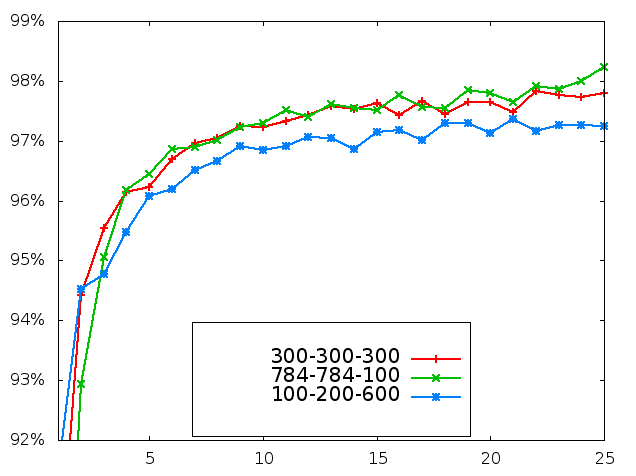
\includegraphics[width=0.6\textwidth]{comp.png}
    \caption{Comparison of the three type of distribution of neurons between layers}
    \label{fig:comp}
\end{figure}


\subsection{Candidates for enhancing}
\label{method}
The most basic method for visualizing a perceptron is cherry-picking those pictures which results in the highest output.
Formally: for a given network and set of input samples, a set of candidates can be found, which yield the highest output w.r.t. each neuron. 
For a given layer, the search can be done parallel, and for more general results, not only the best samples are taken into account, but the top $T$ inputs yielding the highest activation of all samples from the given search set, see Figure \ref{fig:n1}. 
\begin{figure}
    \centering
    \includegraphics[width=0.6\textwidth]{NN1.png}
    \caption{First step of visualizing the $l^{th}$ layer: selecting each neuron's most confident choice from the image set}
    \label{fig:ga-method1}
\end{figure}

\subsection{Enhancing - gradient ascent}

Simply mean averaging the candidates would not reveal the true signals which each neurons look for, see Figure \ref{fig:mean-ga-comp}

\begin{figure}
    \centering
    \includegraphics[width=0.5\textwidth]{mean-ga-comparison.png}
    \caption{On the first set of pictures the mean of the $T=100$ candidates are shown, they are the most preferred inputs of the candidate set for the last layer's neurons. On the set depicted below the enhanced images are shown}
    \label{fig:mean-ga-comp}
\end{figure}
\begin{figure}
    \centering
    \includegraphics[width=0.8\textwidth]{NN2.png}
    \caption{One iteration shown: a hidden layer's weights cannot be reshaped into images, but applying their activation gradient on the input images will emphasize, and amplify the patterns which yields the highest output w.r.t each neuron}
    \label{fig:ga-method2}
\end{figure}
Gradient ascent is an iterative method for enhancing the input to emphasize the patterns that are recognized by the neurons. A method which utilizes a network on top of the original to extract the recognition patterns, called DeConvnet, is described by Zeiler \emph{et al.} \cite{zeiler2014visualizing}. The mentioned algorithm can be reduced to the following, by leaving out the sparsity encouraging regularization term - making parallel processing more efficient:
for fully connected layers the method boils down to backward propagating an \emph{arbitrary} delta vector (instead of calculating the gradient of the loss function described in \cite{zeiler2014visualizing}): 
$\delta_l = \mathbf{e}$ or $\delta_l =\mathbf{b}$
from the $l^{th}$ layer toward the input layer to get gradient of the input w.r.t the $i^{th}$ neuron's activation of the $l^{th}$ layer, and iteratively update the original sample by the gradient multiplied with \emph{modification rate}. The method is depicted on Figure \ref{fig:ga-method1} and \ref{fig:ga-method2}, 
for visual guide for understanding how the applied gradient looks like, see Figure \ref{fig:grad-sub}.

\begin{figure}
    \centering
    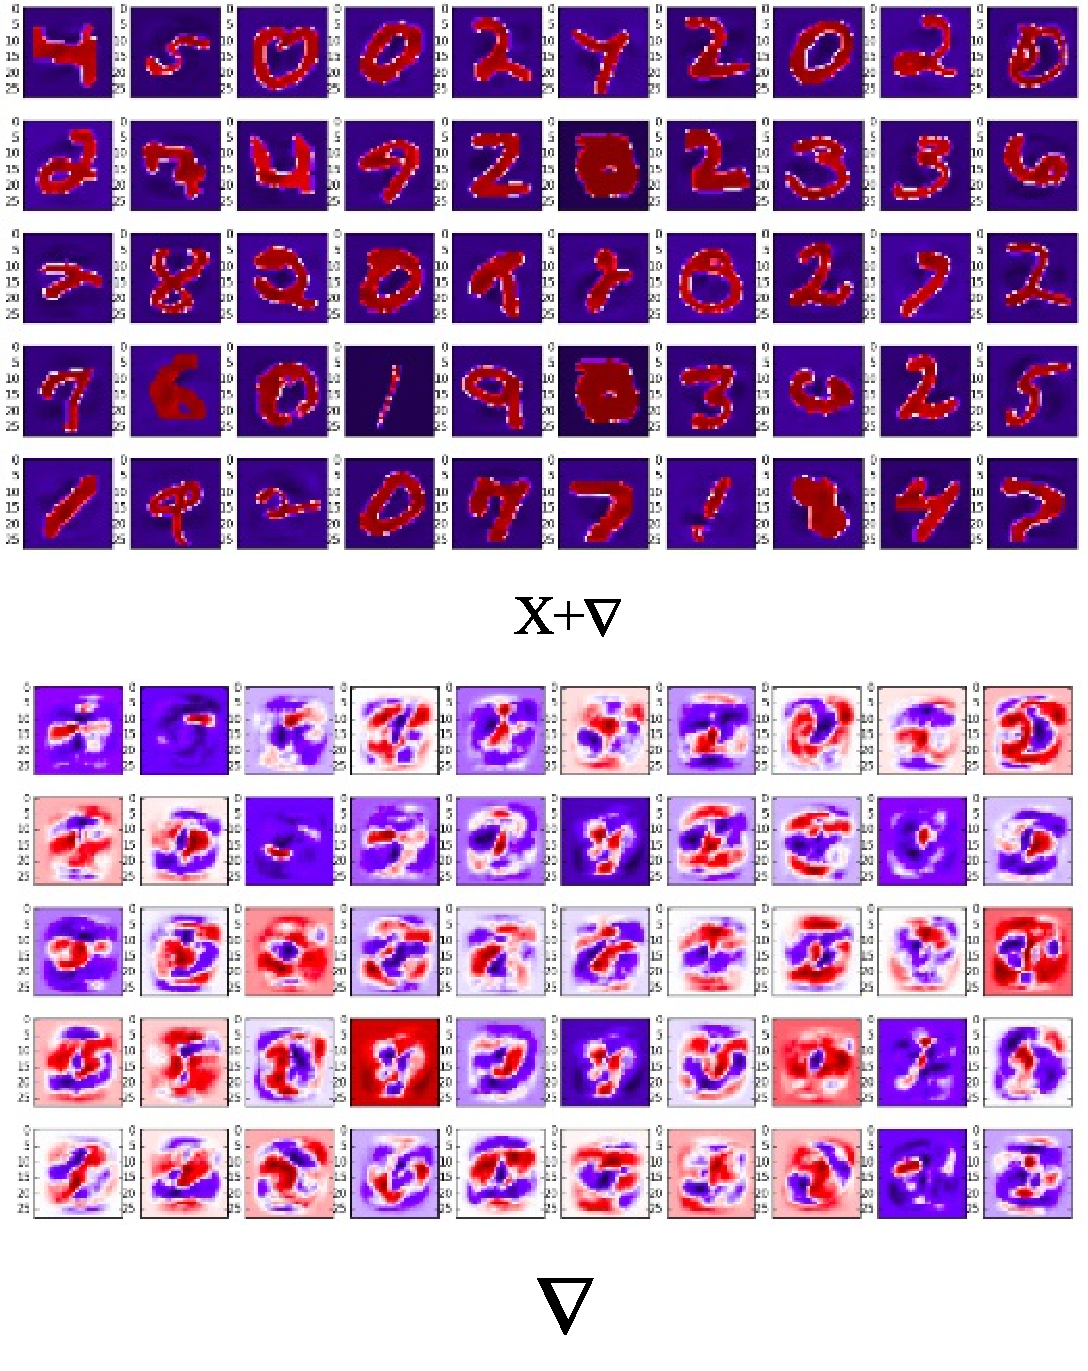
\includegraphics[width=\textwidth]{grad-sub.pdf}
    \caption{After one iteration the enhancement is evanescent, still the gradient holds important information of the layer.
    By looking at the gradient, we can tell which parts will be emphasized and which will be diminished during the process.
    The depicted gradients are extracted from the randomly picked neurons from the first hidden layer of a two layered network.
    For the smooth image result \texttt{bicubic} interpolation was used, with \texttt{seismic} color map.
    }
    \label{fig:bias-nobias}
\end{figure}


By choosing $\mathbf{e}_{i} = [0, 0 \cdots 1 \cdots 0]^T$ the enhancement would not take other activations into account, while letting $\delta_l = \mathbf{b}_i = [-1, -1 \cdots 1 \cdots -1]^T$ would result in activation where other neurons' output would decrease over amplification. 
Both methods were tested by the following procedure: The top 1 digit was selected for each neurons in the last layer of the best performing network, totaling in 10 samples. Skipping the candidate search of the top 10 samples were enhanced by the GA algorithm, with different number of iterations and with $\mathbf{e}$ and $ \mathbf{b}$. The results are shown on Figure \ref{fig:bias-nobias}. 

\begin{figure}
    \centering
    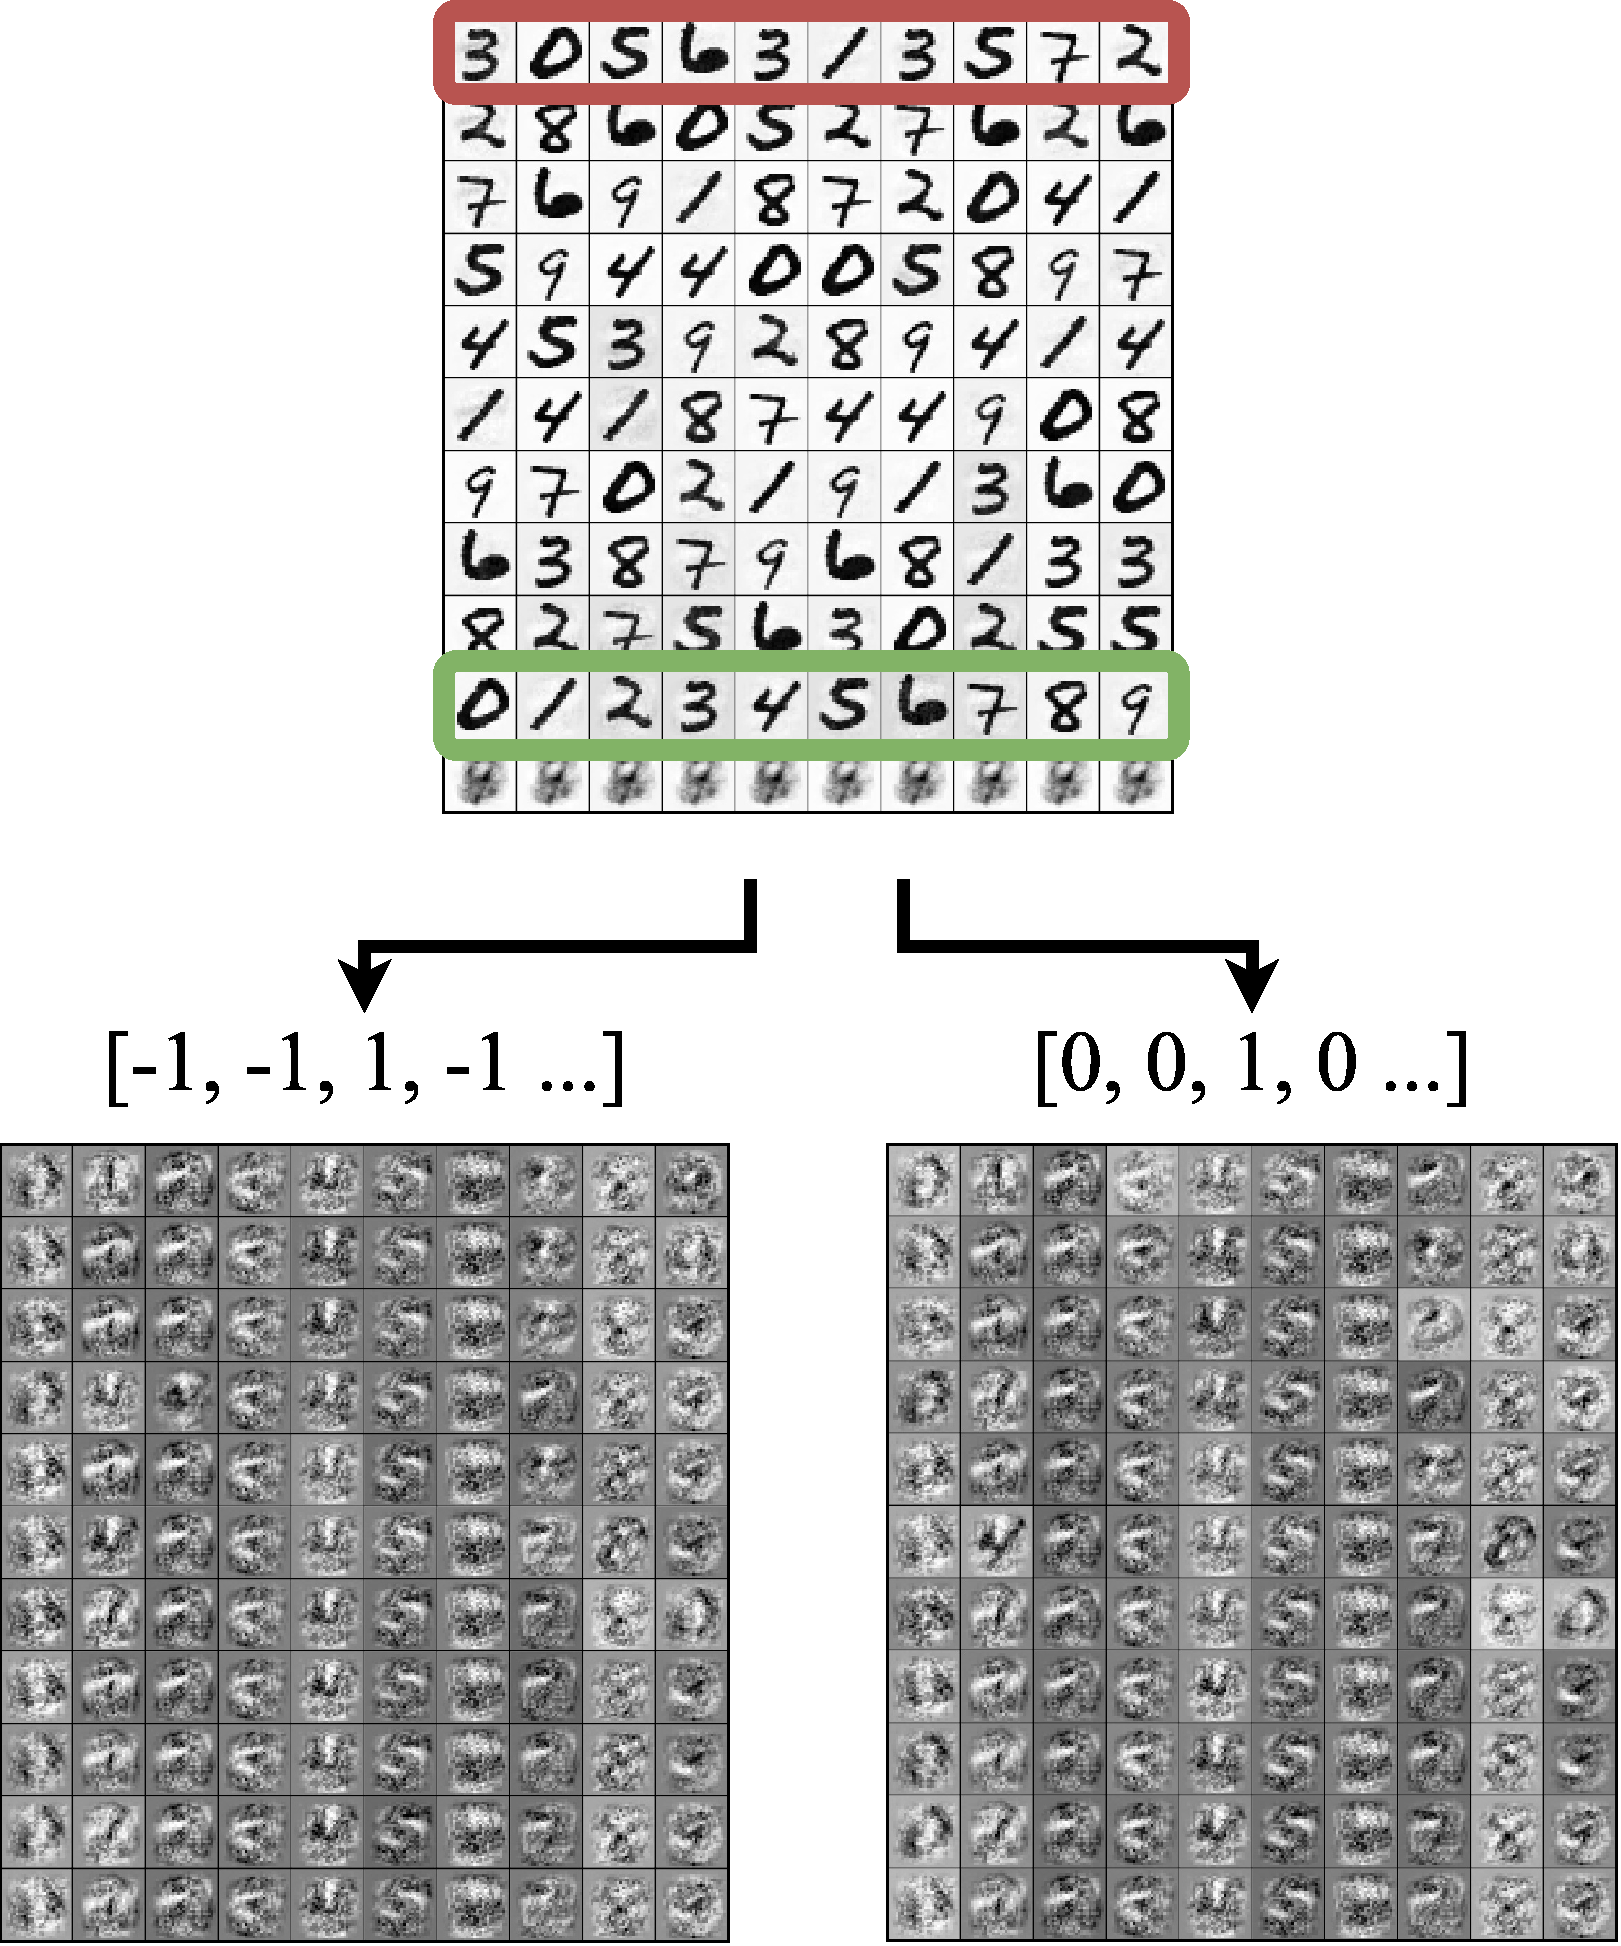
\includegraphics[width=0.9\textwidth]{bias-nobias.pdf}
    \caption{
        The different results of visualizing the last layer of a 3 layered network with 40 iterations of \emph{Gradient Ascent}. 
        Samples highlighted in green are the samples which were recognized with the highest confidence by each classifier perceptron in the last layer.
        These samples are organized in increasing order w.r.t. response of each neuron resulting in a $10 \times 10$ figure.
        \emph{Top diagram (highlighted in red)}: are the samples of the 10 candidate sample which caused the lowest activation.
        \emph{Bottom of the diagram (below the green box)}: there is a row of mean average of the samples above it, for each neuron.
        The arrows are pointing to diagrams, organized in a similar fashion, depicts samples enhanced by 
            G.A. applied with the corresponding gradient on the latent layer. 
        \emph{Left diagram}: samples enhanced by \textbf{biased} GA.
        \emph{Right diagram}: samples enhanced by \textbf{unbiased} GA.
    }
    \label{fig:bias-nobias}
\end{figure}
It is important to notice, that the algorithm initialized with different samples will introduce artifact features on the samples. 
These features will bring closer the input towards an artificial sample which will much more likely be recognized as a sample from the class of the corresponding neuron. 
The method of distortion can be exploited as well, which is called \emph{generating Adversarial} samples (detailed explanation in the end of the section).
However applying GA on the sample with the corresponding neuron (samples in the green box on Figure \ref{fig:bias-nobias}) results in much better visualization of \emph{what each node is looking for} on the input.
By qualitative analysis we concluded that biased Gradient Ascent takes less iterations to transform the sample, however applying it should be  only restricted in the classifying layer, since it is diminishing activation of neighboring neurons. 
A comparison of how the algorithms work iteration by iteration, on noise and misleading samples is shown on Figure \ref{fig:noise-GA}
    

\begin{figure}
    \centering
    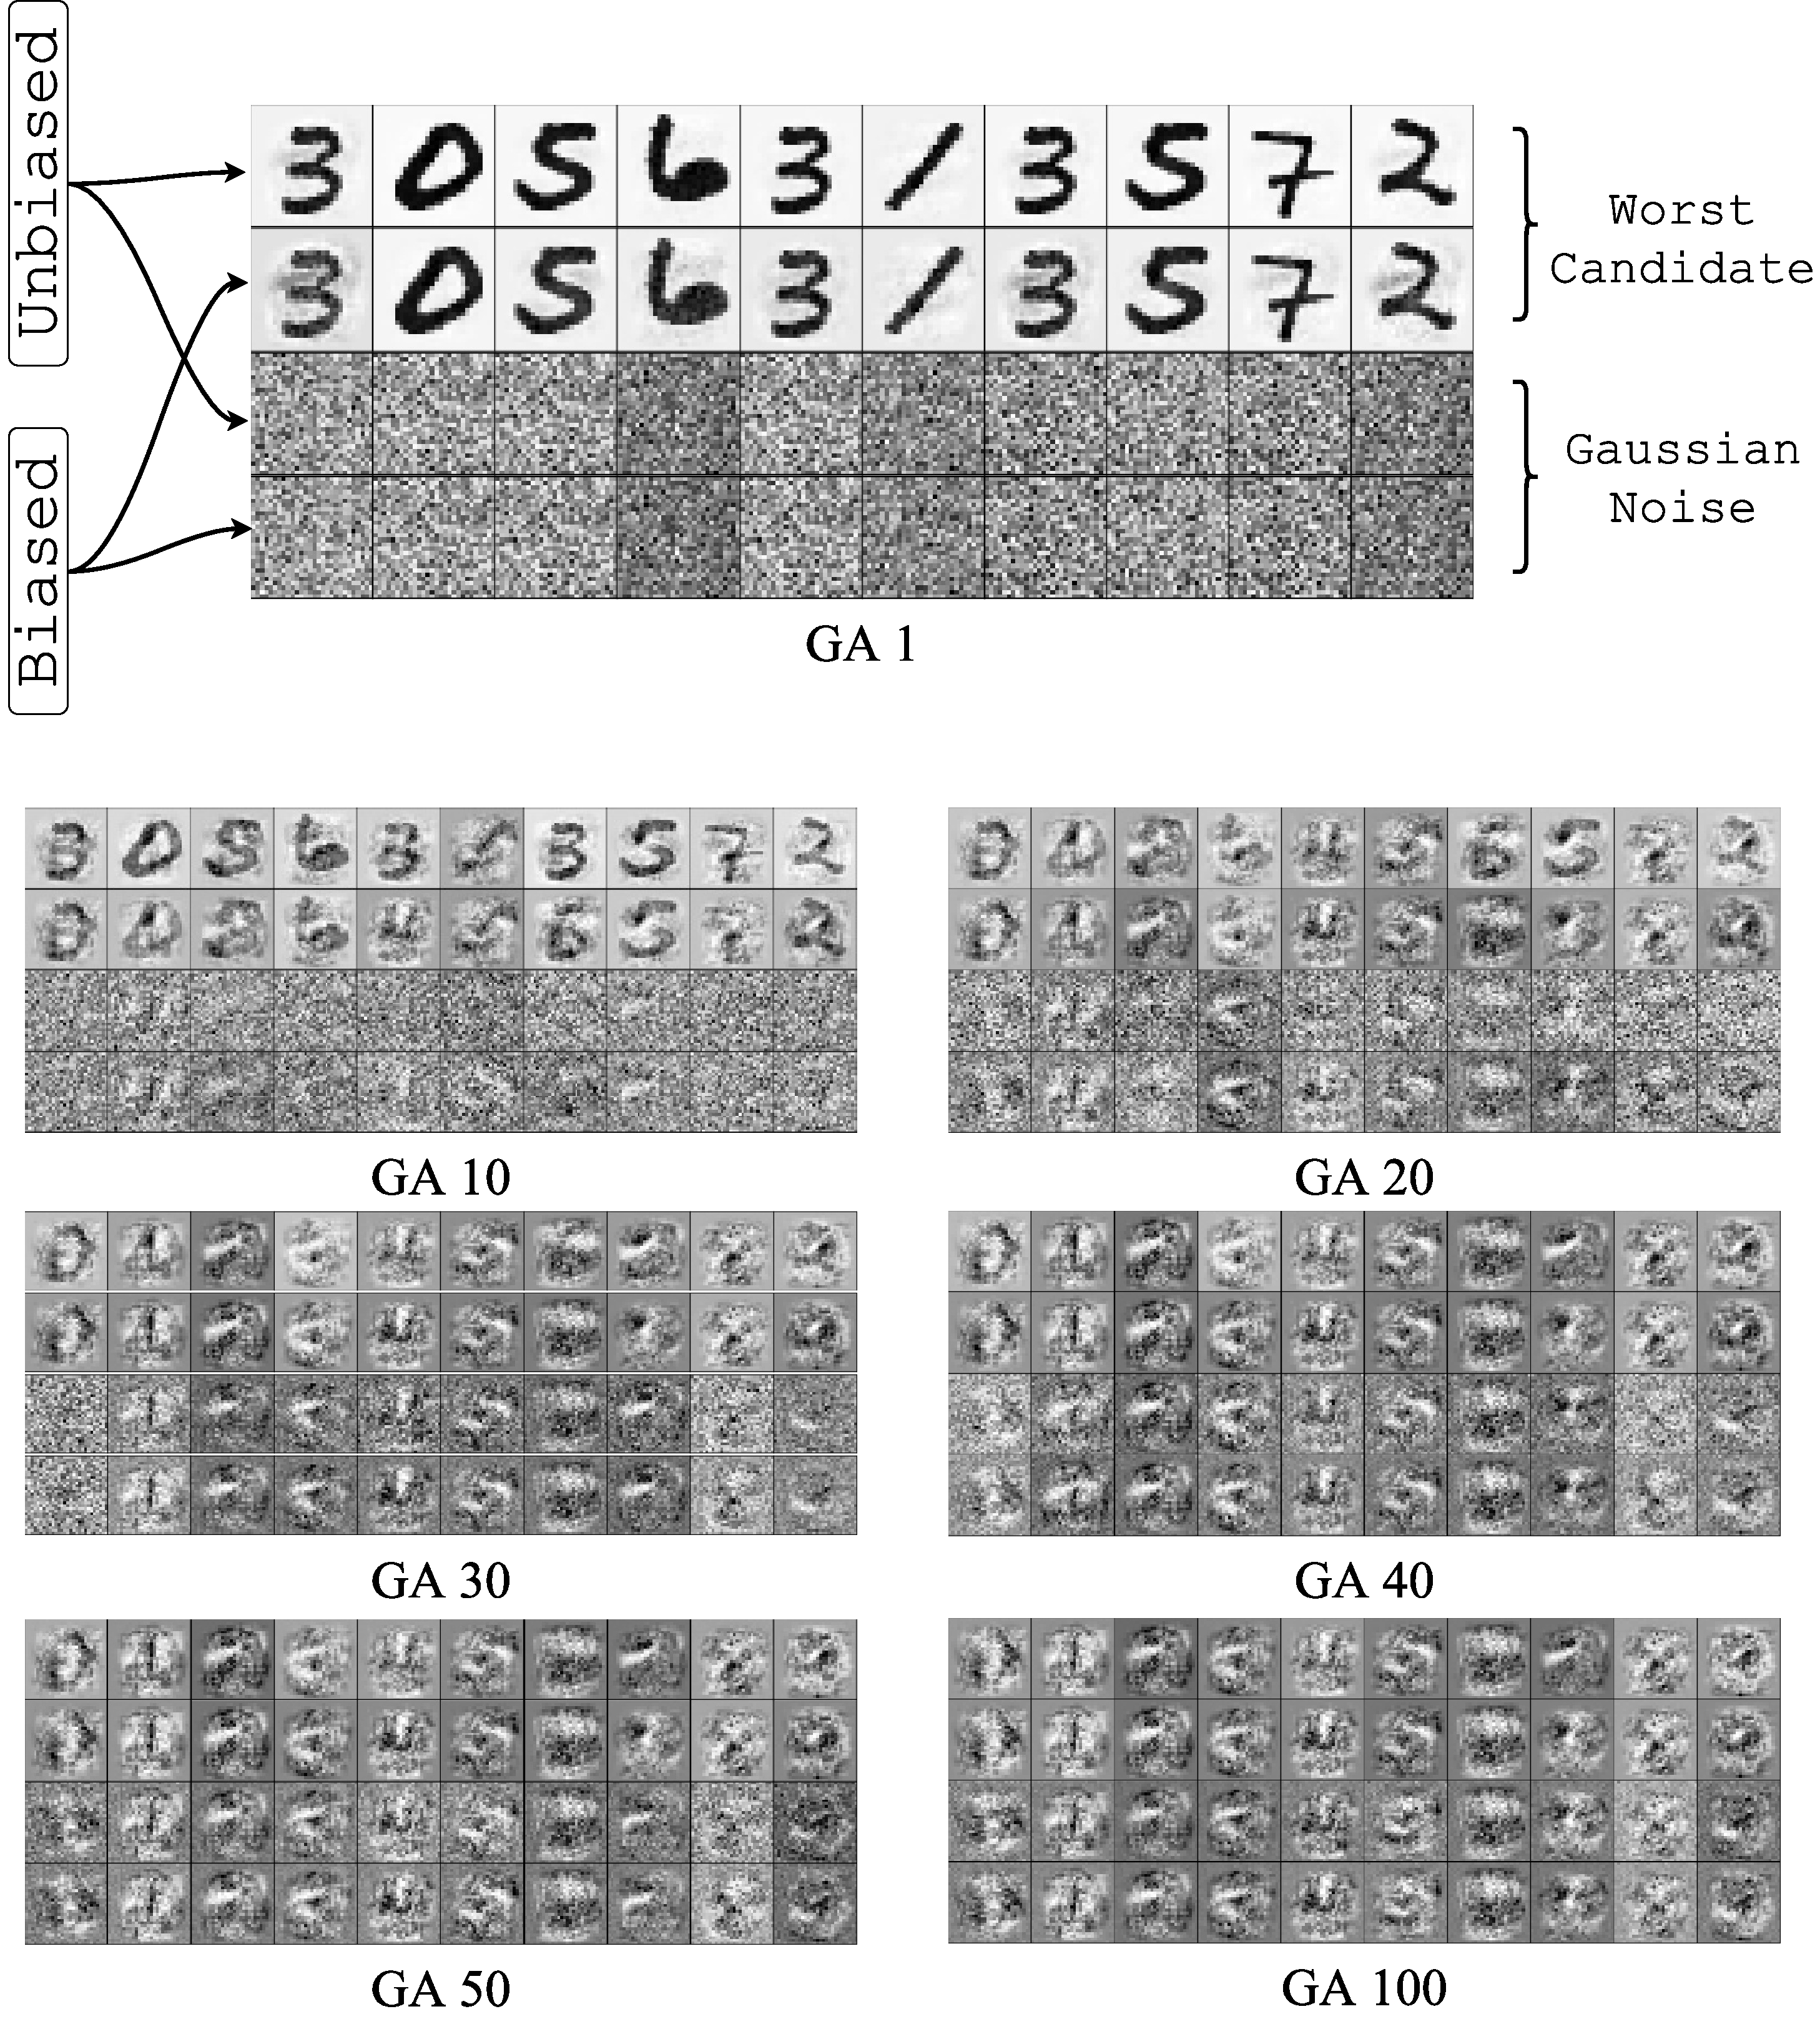
\includegraphics[width=0.9\textwidth]{noise-GA.pdf}
    \caption{...}
    \label{fig:noise-GA}
\end{figure}

Therefore for further analysis $\mathbf{e_i} = [0, 0 \cdots 1 \cdots 0]^T$ is used.
$$x = x + \mathbf{\eta}\cdot\nabla_l^i x$$
Applying the gradient to the input $x$ is the first step of the iteration (see Figure \ref{fig:n2}). Next step is forwarding the enhanced input, applying the $\delta$ on the $l^{th}$ layer and backwarding, and applying it on the input again makes a full cycle.
The hyperparameters of the method are the \emph{rate of amplification $\mathbf{\eta}$} and \emph{number of iterations $I$}

\subsection{Processing enhanced samples}
The results of amplifying the top $T$ samples for $n_l$ number of neurons in the $l^{th}$ layer are stored in a $d + 2$ dimensional matrix:
$$
    shape(\mathbf{R}) = (T, n_l, d_1, d_2, \cdots)
$$
where $d$ is the dimension of the original input.
For compact visualisation, the results are aggregated, mean averaged in the first dimension of $\mathbf{R}$ which highlights the main parts of the input, that took role in increasing the activation of the given neuron.


\subsection{Results of visualization}

A pre-trained network holds generalized information in the weights and biases, and the approach mentioned in \emph{subsection \ref{method}}, produce great amount of possible representations of the networks' inner state. In this subsection MNIST samples enhanced by parameters derived from the \emph{MLP}s trained in \emph{subsection \ref{train}} are analyzed and compared - \textit{absolutely} non exhaustively, following intuitions like:

\begin{itemize}
    \item Where, and how does abstraction occur, from combining previous layers' activation patterns
    \item How does differently distributed nodes affect the above.
    \item Do fully connected networks converge to recognizing \emph{localized} patterns, like convolutional networks do
\end{itemize}

\subsection{Challenges} Because the parameter space is too wide, the main obstacle in visualization is to find out what to look for. For example visualizing the current best network that has the following dimensions: 
\begin{itemize}
    \item for each node in the network there is a $T \times 28 \times 28$ sized input set
    \item for each layer there is a given set of nodes $N = [784, 784, 100, 10]$ respectively
\end{itemize}

Totaling in $T\times(N_l)$ picture per layer, which are hard to deal with, \emph{(see Figure \ref{fig:dense})}. 
Especially when the neuron's favored patterns can be matched to different digits, 
the $T$ should be increased in order to get a more general picture when aggregating the amplified pictures.
On the other hand, the gradient ascent optimization cannot terminate on \emph{convex functions}, which is actually true for the activation of neural node's activation w.r.t to its input - meaning that the original image can be amplified as many times as possible, the output of the corresponding neuron $y_l^i$ will always increase with the number of iterations $I$. An example for applying the same method, but with 5 times the original number of iterations depicted on \emph{Figure \ref{fig:dense}} is shown on \emph{Figure \ref{fig:dense-100}}.
Therefore finding the best $I$ is also essential for extracting important information from the network.


\begin{figure}
    \centering
    \includegraphics[width=0.6\textwidth]{mean-noGA.png}
    \caption{The naive way to extract interpretable patterns is to gather those inputs which excites the most the given layer, and \textbf{mean average} it. The case depicted on the figure, is that the ideal input is not trivial as the listed candidates shows, especially in the first layers. By aggregating}
    \label{fig:mean}
\end{figure}


\begin{figure}
    \centering
    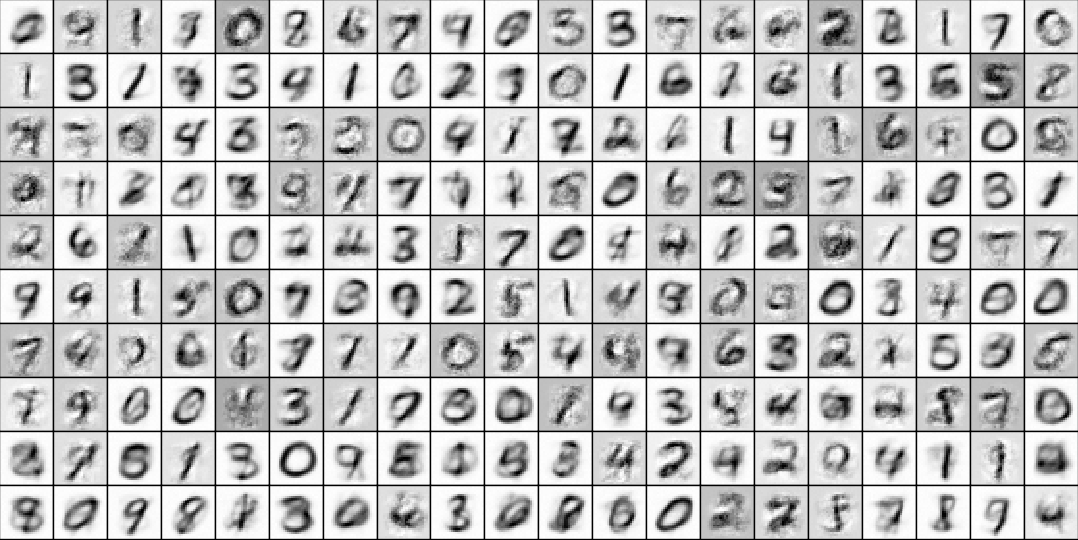
\includegraphics[width=0.9\textwidth]{200-dense-GA20.png}
    \caption{Iteratively enhanced pictures of the first hidden layer of a \textbf{[300-300-300]} network (first 200 are shown in \emph{row-major order}). The main question is, which of them holds important features, or needs further analysis.}
    \label{fig:dense}
\end{figure}


\begin{figure}
    \centering
    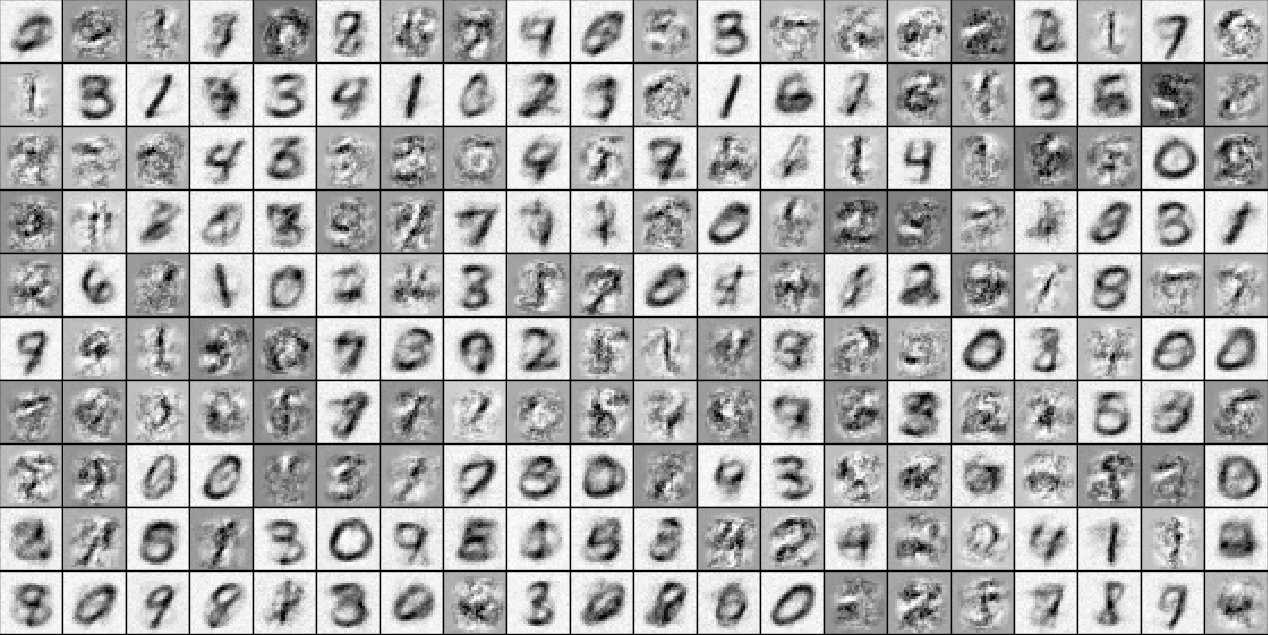
\includegraphics[width=0.9\textwidth]{200-dense-GA100.png}
    \caption{After increasing $T$, compared to fig. \ref{fig:dense} some of the amplified pictures gets noisy, which is not a problem in the first case. It is a trend in the early layers, to only focus on small, localized type of features, that yields different candidates, which makes the mean of the outcome noisy overall. Especially this is one important feature of \emph{MLPs} that initialized with random weights they converge towards recognizing localized features.}
    \label{fig:dense-100}
\end{figure}


\emph{\textbf{Note}: Deviating, or averaging the input samples is an important step to strengthen the features which the given node truly recognize, and drop out those which it does not (see Figure \ref{fig:mean}). For the rest of the case studies mean averaging is used for aggregation}

\textbf{Remainder}: For the following examples, a small subset of samples are shown, which were selected for the most revealing clues. Still, they may not represent all features of the network.


\subsection{Analyzing the best performing network}
The best result belongs to a network with hidden layer width: 784-784-100. 
The layers were visualized with the following parameters:
$T=100$
$\eta=0.1$
$I=10, 50$
and the training set was used for choosing candidates.

The suggestion while looking for evidences is that the reason behind the good performance of the network is relying on different levels of abstraction.
I visualized all three layers in order to get a better grasp what happens inside of a network, which can recognize digits with $98\%$ success.
For conviction, that we cannot simply read the values out from neither the activation, or the weights from the hidden layers see Figure \ref{fig:act-weight}.



\begin{figure}
    \centering
    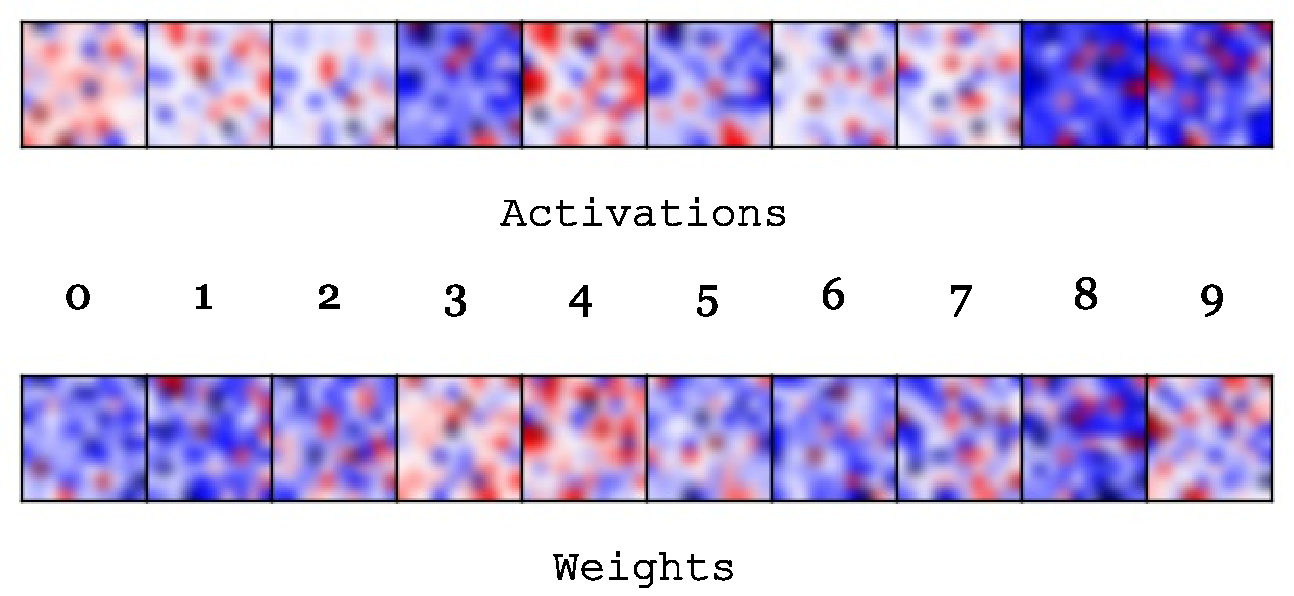
\includegraphics[width=0.9\textwidth]{act-weight.pdf}
    \caption{\emph{On top}: Every sample translates to some response signal (like the depicted maps) before reaching the final classifier layer. 
    Though we cannot understand it, for the network the activation patterns holds all information about the corresponding input.
    \emph{On bottom}: Each map is processed by the weights of the last layer, which is also essential for the network, but does not exhibit any intuitive feature.
    Think about the analogy: we cannot simply define what happens inside by just looking at brains of creatures. 
    Even if we had a high resolution microscope, revealing the fine structure of the nervous tissue would not suddenly illuminate everything.
    }
    \label{fig:act-weight}
\end{figure}
\clearpage
		%
\clearpage
\chapter{Conclusion}		%
\clearpage

%% TARTALOM
%%%%%%%%%%%%%%%%%%%%%%%%%%%%%%%
%% BEFEJEZÉS

\chapter{Summary}

In this work I provide a detailed introduction of building feed-forward neural networks, supported by both illustrative examples and mathematical proofs. 
The examples are based on biological motivations, and practical applications of NN. 
In the \textbf{Design and Implementation} chapter I present a guide to understanding and writing the neural network framework step-by-step, which I used to produce results in \textbf{Case Studies}. 
The newest implementation can be find at \cite{DV}, supported with out-of-the-box demo scripts, and \texttt{ipython notebooks}.
The library is modular in the first place, and easy to utilize because of the layer manager functions of the \texttt{network} class found in the \url{network_module}. 
It is also easy to \emph{fork} the implementation, and join the further development of the framework -- the phases of improvement are well documented, thanks to the version control supported by Git, and synchronized on the GitHub repository.

By working on this project I have understood the main concepts of Machine Learning, and experimented with multiple design patterns on how to realize the inference \ref{eq:forward} and backpropagation \ref{backprop} functions and arrived at the best fitting design: 
object-oriented implementation of \textbf{layers} handling the lattices of the computational graph derived from the abstract layer and \textbf{networks} managing the organization and training of layers.
My implementation offers both user-friendly interface and opportunity to fine-tune the network with advanced parameters as optional arguments.

I have utilized and tested the network on different tasks of popular Machine Learning problems, namely \textbf{Voice Recognition}, and \textbf{Image Classification}.
I was not just able to reproduce results of other researchers but I have also produced unique results;
while studying novel techniques of revealing perceptive fields and favored patterns of neurons, 
I have developed my own method for visualization by altering the backpropagation function of layers, arriving at the biased and unbiased \textbf{Gradient Ascent}.
I made experiments on the effects of GA, and studied how different shaped networks infer the input data, also how they could be exploited to make adversarial inputs. In a nutshell the results are the following: unbiased GA should be used for transforming samples into inputs which fools classifying networks, and biased GA for enhancing multiple samples to extract patterns from neural networks. The details of the experiments are explained in \textbf{\nameref{sec:MNIST}} section.
		%
\clearpage
\chapter{Future}

\paragraph{Short-term plans.} 
Currently I have a working version of the convolutional layer, 
however the implementation still relies on \texttt{convolve2d} function of ScyPy, which slows down the training process.
In the following months I will work on my own implementation of the convolution function, 
and improve the network usability.
Recently I have been able to train my network on CIFAR~\cite{cifar}, and ImageNET~\cite{deng2009imagenet} dataset, and the results are encouraging, however not enough yet to publish.
I am also working on \emph{Restrictive Boltzmann Machines} to be able to build and make experiments of \emph{Deep Belief} networks.

I am very interested in fields of \emph{Reinforcement Learning}, 
and I plan to utilize a network that plays the popular game, \texttt{agar-io}.
Also I am currently studying \emph{Recurrent Neural Networks} especially implementations of \emph{Long Short-Term Memory} architectures, 
which are not just better for audio recognition tasks, but can be used as Generative networks, producing artificial samples.
I want to create an application capable of accompanying musicians in jam-sessions, based on \emph{LSTM} networks.
I will continue my studies in field of \emph{Generative Adversarial Networks} which is currently a very hot topic of Computer Vision.

\paragraph{Long-term plans}
My studies have two basic motivation:
When observing living organisms I think about how could we model them, 
and reverse-engineer their function.
I want to contribute with my own studies to the current level of Artificial Intelligence.
On the other hand, via visualization I want to get closer to understand our 
environment and how can we build knowledge based on our experiences.
			%
\clearpage

\printbibliography
\addcontentsline{toc}{chapter}{Bibliography}
%% BEFEJEZÉS
%%%%%%%%%%%%%%%%%%%%%%%%%%%%%%%
\end{document}